\documentclass[a4paper,10pt,twocolumn]{amsart}

\usepackage{osnova}


\newcommand{\ans}{\it{�����: }}
%��� �������
\newcommand{\htext}[1]{\par{}}
\newcommand{\hans}[1]{\par{}}

%������
%\newcommand{\htext}[1]{#1}
%\newcommand{\hans}[1]{\par{\ans $#1$}}

\title{������ ��� ���������� �  ���2015.}

\begin{document}

%\twocolumn[ \maketitle ] \tableofcontents
%\parindent=0cm

\newpage
 \twocolumn[\section*{ ������� 1 ���2016.}]\setcounter{z}{0}

\zad
����� ����� 7 ������ 60 ������. ����� ���������� ����� ������ ����� ������ �� 60 ������?

\zad
�������� ��������� �� 1000 ���������� � 30 ������ �������. ������ ������������ ������ ����� �������� 50 �������. ����� ���������� ����� ������ ������ ���� �� ���������, ����� � ������ ������������� � ��� ����� ���� ���������� ���� ���������� � ���� ������ �������?


\zad
������ ������� ����� 200 ������. ����� ���������� ����� �������� ����� ������ �� 1000 ������ �� ����� ����������, ����� ������ ���������� 15\% ?


\zad
��������� ����� ����� 30 ������. ����� ���������� ����� ����� ����� ����� ����� ������ �� 700 ������ ����� ��������� ���� �� 25\% ?


\zad
������� ����� 40 ������. ����� ���������� ����� ����� �������� ����� ����� ������ �� 750 ������ ����� ��������� ���� �� 10\% ?



\zad
������ ���� � ����� ������ 6000 ������ �� ��� ��� 15 \%. �� ������ �������� ������, ����� � ���� ���������� ���������� ����� �����, � ��� ����� ����� ��� ��������� ��� �����, ������ � ������, ������ � ����������. ������� ������ �� ������ ������� � ���� ����������?


\zad
� ������ ������ �� ������� ��������� ���������� 70 � ������ � ����. � ������ 163 ��������. ������� ������������� ����� ������ ����������� �� ���� ������ �� 7 ����?


\zad
� ������ ������ 249 ����� � 28 ������������. � ������� ���������� �� ����� 45 ����������. ������� ��������� ���������, ����� ��������� ���� �� ������ � �����?


\zad
����� ��������� �������� ����� 90 ������. ���� ������ 1 �� 800 � ��������. ������� ������ ����� ��� ������ �������� � 500 ������?

\zad ����� �������� ����� ������������ ����������, ��������� �������� ���������� �������� � ����� � ���.
������������ ���� ����� 1609 �. ������ �������� ���������� � ���������� � ���, ���� ��������� ���������� 33 ���� � ���? ����� ��������� �� ������ �����.

\zad  ����� �� ������ ���������� 13\% �� ���������� �����. ����� ��������� ������ �� ������ ����� �������������� �������� 9570 ������.
������� ������ ���������� ���������� ����� ����� ��������������?

\zad
������� �������� ��������� ������ �� ������� ���� 120 ������ �� ����� � ������� � �������� 20\%. ����� ���������� ����� ����� ������� ����� ������ � ���� �������� �� 1000 ������?

\zad
� ����� 500 ������ ������ ������� �4. �� ������ � ����� ����������� 1200 ������. ����� ���������� ���������� ����� ������ ����� ������ � ���� �� 4 ������?

\zad
��� ������ ��������� ����� �� ����� � ������� �� ����� 41 �������. ������� ������ ��� ����������, ���� ��������� ����� �� ����� ����� 580 ������, � ������� ������� � 20 ������?

\zad
�������� ��������� ���������, ������� ����� ���� �� 0,5 � 3 ���� � ���� � ������� 21 ���. � ����� �������� 10 �������� ��������� �� 0,5 �. ������ ����������� ���������� �������� ������ �� ���� ���� �������?

\zad
��� ������������� �������� ��� ������� �� 1 ���� ���� ��������� 12 � �������� �������. �������� ������� ��������� � ��������� �� 10 �. ����� ���������� ����� ����� ����� ������ ������� ��� ������������� 6 ������ ��������?

\zad
��������� ����� 35 ������. � ����������� � ������������ ��������� ����������� �����������: �������� �� ��� ���������, ���������� �������� ��� (���� � �������). ������� ��������� ����� �������� �� 200 ������ � �����������?

\zad
������� ���� �������� 170 ������. ��������� ���� �� 20\% ���� �������. ����� ���������� ����� ����� ��������� ����� ������ �� ��������� ���� �� 7000 ������?

\zad
��������������� ����� ��� ��������� ����� 720 ������. ��������� ������ ��� ��������� ���������� 50\% �� ��������� ������ ��� ���������. ������ ������� �� 15 ���������� � 2 ��������. ������� ������ ����� ������ �� ��� ������?

\zad
���� �� ������������� ������ ���� �������� �� 16\% � ��������� 3480 ������. ������� ������ ����� ������ �� ��������� ����?

\zad
�������� ������ 800 ������. ����� �������� ���� ��� ����� ������ 680 ������. �� ������� ��������� ���� ������� ���� �� ��������?

\zad
� ������ $N$ ����� 200000 �������. ����� ���  15\% ����� � ����������. ����� �������� ������� 45\% �� �������� (����������, ��������, ����������� � �.�.). ������� �������� ������� ��������?

\zad
������� �� ����� ������� 6000 ��. ��������� 1 ����� ������� --- 20 ������. ������� ������ ������� �� 100 �� ���������� 9 ������. ������� ������ �������� ������� �� ������ �� ���� �����?


\zad
�� ���� �������� ���������� ������ ����� �� ��������� ����� ������. �������� ����� 30 ������ �� �����. � ���� ���� 500 ������. �� ������ ����������� ����� ��������� �� ����� ������ ����� ���� �� ���� ��������?

\zad
� ��������������� ���������� �������� ����� �������� �� ��������� ��� 1-3 ������, �� 360 ���� ��� ������� �����. ��� ����� ��������� �� �������. � ������� ����� 9 �����, �� ������ ����� ����������  25 ���������. ������� ������ ����� ��������� ��������� ������ ����������?

\zad
��� ������������� ��������� ������� �� 1 �� ����� ����� 1,5 �� ������. ������� ������������� �������� ������ ����� ������, ����� ������� ������� �� 27 �� �����?

\zad
��������� ���� �������� 180 ������, ��� �� 20\% ���� ������� ����. ����� ���������� ����� ����� ��������� ����� ������ �� ������� ���� �� 10000 ������?

\zad
�� ����� �������� ���������� �������� ���� 53 �����, � ����� ��������� � ����� �������� 8 ������. ������� ����� ������ �������� � �����, ���� ���� ������ ��������� ����� 2 ����� 50 ������.

\zad
���������� 11 "�" �������� ������ ������ ��� ���������� ������: �� 3 ��� ������� ������� � �� 7 ��� ��������� ������������ � ���������. ��� ���������� �������� ������ 15 �������� (������� ��������� � ��������� ������������), ���� ���������� �� ������� ���� 35 ������ �� �����. ������� ������ ����� ��� ����?

\zad
1 ��������-��� �������������� ����� 1 ����� 80 ������. ������� �������������� 1 ������ ��������� 12625 ��������-�����, � 1 ������� ��������� 12802 ��������-����. ������� ������ ����� ��������� �� �������������� �� ������?

\zad
� �������� ������ 1 ������ ����� 3 ����� 70 ������. ���������� �������� ����� �� ������ � ������ 3 �� ��������� �� ���� 4 ������ �� 1 ��. �� ������� ������ �������� �� ��� �������? ����� ��������� �� ������ �����.

\zad
���� ��������� SMS-��������� � ����������� �������������� ����� 16 �������. ��������� ������ SMS-��������� 1 ����� 30 ������. ����� ��������� ��������� �� ����� � ���� ���� 30 ������. ������� ������ ��������� � ���� ����� �������� ���� ���������?

\zad
����� �����������-���������� ������������ � $15:20$, � ��������� � $4:20$ �� ��������� ���� (����� ����������). ������� ����� ����� ��������� � ����?

\zad
� ����� ���� ����������� ������������� �������. ����� ���������� ����� ������� ����� ����� � �����, � ������� ��������� 20 �������?

\zad
� ��������� ��������� � ������ ������� ����� �������� ������� �������. ����� ���������� ���������� ������ ���������� ��� ��������� 83 ����������� ���������?

\zad
������ ���� �� ����� ����������� ����������� 70 ��������� ���. ����������� ������ 6 ����. ��� ��������� � ������ �� 50 ���������. ������� ����� ����� ������ �� ��� ��� �����������?

\zad
� ����� 124 ������� ������� ����������� ����, ��� ���������� 25\% �� ����� ���� ��������. ������� �������� ������ � �����?

\zad
27 ����������� ����� ���������� ������� � ����������� �����. ��� ���������� 30\% �� ����� �����������. ������� � ����� �����������?

\zad
����� ���������� ����� ����� 60 ������. ����������� ������� ������ ������ 5\%. ������� ������ �������� ��������� �� ����� �����?

\zad
������� ����� 24 �����. ������� ������ �������� ���������� �� 60 ��������, ���� ��� ������� ������ 50 �������� ������� ������ ������ 10\% �� ��������� ���� �������?

\zad
��������� ��������� ��������� �� ���������� ����� 48 ��������, ��� ��������� 12\% �� ����� ����������. ������� ������� ����������� � ���������?

\zad
������ 94\% �� 27500 ����������� ������ ��������� ������ ������ B1. ������� ������� ��������� ������ ������ �1?

\zad
��������� ������� ����� 3500 ������. ����� ��������� ����� ���� �� ��� ������ ������� �� 2800 ������. �� ������� ��������� ���� ������� ����?

\zad
� ����� 800 ��������, �� ��� 30\%  --- ������� ��������� �����. ����� �������� ������� � ������� ����� 20\% ������� �������� ����. ������� �������� � ����� ������� �������� ����, ���� � ��������� ����� �������� ���� �� ���������?

\zad
����� 40000 ������� ������ 60\% �� ������������ ��������. ����� ���������� ����������� 80\% �������� �� ���������� ����� ���� ���������. ������� ������� ������ �������� ���� ���� �� ����������?

\zad
� �������� 1 �� ��������� ����� 60 ������, � ������� �������� ��������� �� 25\%, � � ������ ��� �� 20\%. ������� ������ ����� 1 �� ��������� ����� ����������� � ������?

\zad
� ����, � ������� ����� ����, ���� �������. �� ������ ����� �� ����� �������. ���� ����� � �������� 50. �� ����� ����� ����� ����?

\zad
� ����, � ������� ����� ����, 9 ������ � ��������� ���������. �� ������ ����� ��������� �� 4 ��������. ���� ����� � �������� �130. � ����� �������� ����� ����?

\zad
��� ������ ����� ����� ��������� �������� ��������� �������� 5\%. �������� ��������� ����� ������� 10 ������. ��� ����� �������� �� ���� ������ ���������� �������� �� ������ 300 ������. ����� ����������� ����� ��� ������ �������� � �������� ���������� ������� ���������?

\zad
� �������� 1 �� ���� ����� 60 ������. � ������� ����� ���������� �� 25\%. ������� ������ ����� 1 �� ���� ����� ����������� � �������?

\zad
������� ������ ����������� ������ �� ������������ ���������� ��������� �� ���� �������. ����� ������ ����� � �������� 40 ������. ��������� �������� �� ����� ������ 38 ������. ������� ��������� ���������� ������ ��� �����������?

\zad
������� ������� ���� ������ ������� � ������� 700 ������ �� ����������� �������. �� ����� �� ��� ���������� ������ ������ ����� ��������� ��� ����� ����������� ����������� �����. ����� ���������� ���������� ��������� ������ ������ �������, ���� ���������� � ���� ����� �� ������ ���������� 13\% ��������, �������� ����� 60 ������ �� ����� � ����� ������ �������� �� ��������� ����� ������?

\zad
��������� ���������� ���������� �������� � ����� � ���. ����� �������� (� ����� � ���) ���������� ���������, ���� ���������� �������� �� ��������� 36 �� � ���? (��������, ��� 1 ���� ����� 1,6 ��.)

\zad
��������� ���������� ����� �������� �������� �������� ��� ������� ������ 5\%. ����� ����� 200 ������. ������� ������ �������� ��������� ���������� ����� �� ��� �����?

\zad (� 282865)
�� ������������ ������ ����� ������� 1000 ������ � ����� � ��� 32 ����� ������� �� ���� 26 ���. 50 ���. �� ����. ������� ������ ����� �� ������ �������� � �������?

\zad (� 282965)
�� ������������ ������ ����� ������� 1000 ������ � �������� ������ ������ �� ������� ����. ���� ������� 28 ���. 50 ���. ����� ������ ������� 2 ���. 50 ���. ������� ������ ������� ���� ������ � ���?

\zad (� 314877)
� ��������, ��� ��������� ������, ���������� ������ ����� ������� �������� ���� (�������). 1 ���� ������� ��������� ������ 153 ���.� ����, � 1 ���� --- 161 ���.�. ����� ����� ������ ��������� ������ �� �������� ���� �� ����, ���� ���� 1 ���.� �������� ���� ���������� 7 ���. 70 ���.? ����� ����� � ������.

\zad (� 314971)
���� �������� ��������� ����� 40 �� � �������� 7\% ��������� ��������. ������ � �������� �� 6 ������� ���� ����������� 1,4 �� ��������� �������� �� ������ ��������� ���� � �����. ������� �������� ����� ��������� ������� ���� ������ � �������� ������ ������� � ����� 6 �� � ������� �����?

\zad (� 318587)
��������� ������ ���������� ����� 109 ������. �������� ��������� ������ � �����������, ���� � ����� ����� 2,54 ��. ��������� ��������� �� ������ ����� �����������.

\zad (� 318685)
���� ����� 6 ����� 8 ������. �������� ���� ����� � �����������, ���� 1 ��� ����� 0,305 �, � 1 ���� ����� 2,54 ��. ��������� ��������� �� ������ ����� �����������.

\zad (� 318749)
����� �������� 200 � �� 20 ������. ������� ������� �������� ������ �� ���������. ����� ����� � ���������� � ���.

\zad (� 318755)
����� �������� 400 � �� 45 ������. ������� ������� �������� ������ �� ���������. ����� ����� � ���������� � ���.

\zad (� 318761)
� ����� ����� ��������� "������� ������� ��������" ������� ������ ������ � �����������. ��� ������ �� 8 ������� ������� ����� $\dfrac{3}{4}$  ����� ����������. ������� ������� ���������� ������� ����� ��� ������, ������������� �� 4 �������? ��������, ��� 1 ���� ����� 0,4 ��.

\zad (� 318859)
������� ���������, ���������� � ������ ����������� ������, ����������� ��������� � ���, ��� ����� �������� �� ������ 30870 �����. �������� ������ ������ � ������. ��������, ��� 1 ��� ����� 30,5 ��.

\newpage
  \onecolumn \section*{ ������� 2 ���2016.}\setcounter{z}{0}

\zad (� 5327)
�� ������� �������� ��������� ����������� ������� �� ���������� ���� �����. �� ����������� ����������� ���� � ����� �����, �� ��������� --- �������� ����������� � �������� �������. ���������� �� ������� ���������� ����������� ������� 22 ������. ����� ����� � �������� �������.

\begin{center}
 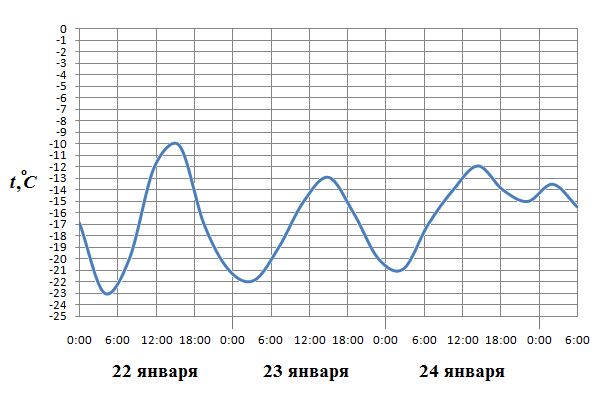
\includegraphics[scale=0.6]{img512717n1.png}
 % img512717n1.png: 608x415 pixel, 72dpi, 21.45x14.64 cm, bb=0 0 608 415
\end{center}


\zad (� 5347)
�� ������� �������� ��������� ����������� ������� �� ���������� ���� �����. �� ����������� ����������� ���� � ����� �����, �� ��������� � �������� ����������� � �������� �������. ���������� �� ������� �������� ����� ���������� � ���������� ������������ ������� 15 ����. ����� ����� � �������� �������.

\begin{center}
 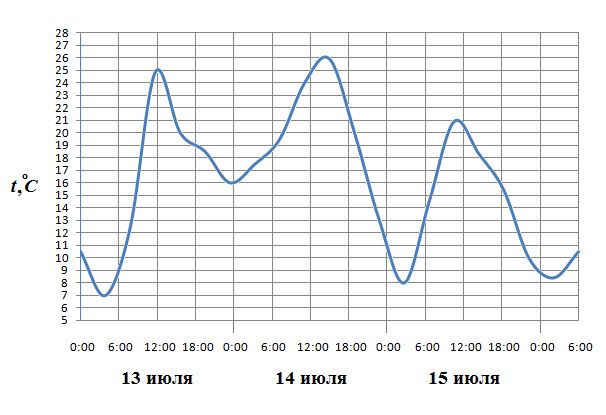
\includegraphics[scale=0.6]{img512737n1.png}
 % img512737n1.png: 606x415 pixel, 72dpi, 21.38x14.64 cm, bb=0 0 606 415
\end{center}


\zad (� 18875)
�� ��������� �������� �������������� ����������� ������� � ����������� �� ������ ����� 1988 ����. �� ����������� ����������� ������, �� ��������� - ����������� � �������� �������. ���������� �� ���������, ������� ���� �������, ����� �������������� ����������� ��������� 20 �������� ������� � 1988 ����.

\begin{center}
 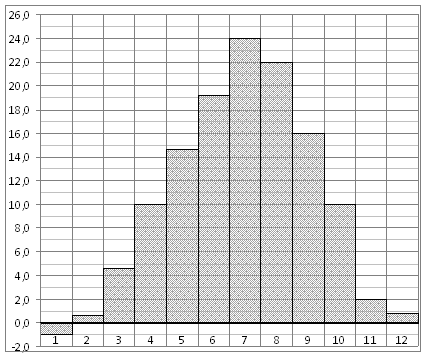
\includegraphics[scale=0.6]{innerimg0.png}
 % innerimg0.png: 425x356 pixel, 72dpi, 14.99x12.56 cm, bb=0 0 425 356
\end{center}

\zad (� 26863)
�� ������� ���������� ����������� ��������� ������� ��������� �� ����� ��� �������� � ������. �� ��� ������� ������������� ����� �������� � ������, �� ��� ������� --- �������� ������ � H$\cdot$�. �������� ���������� (� ��/�) ����������� ���������� �������� $v=0,036n$, ��� $n$ --- ����� �������� ��������� � ������. � ����� ���������� ��������� ������ ��������� ����������, ����� �������� ������ ��� �� ������ 120 �$\cdot$�? ����� ����� � ���������� � ���.
\begin{center}
 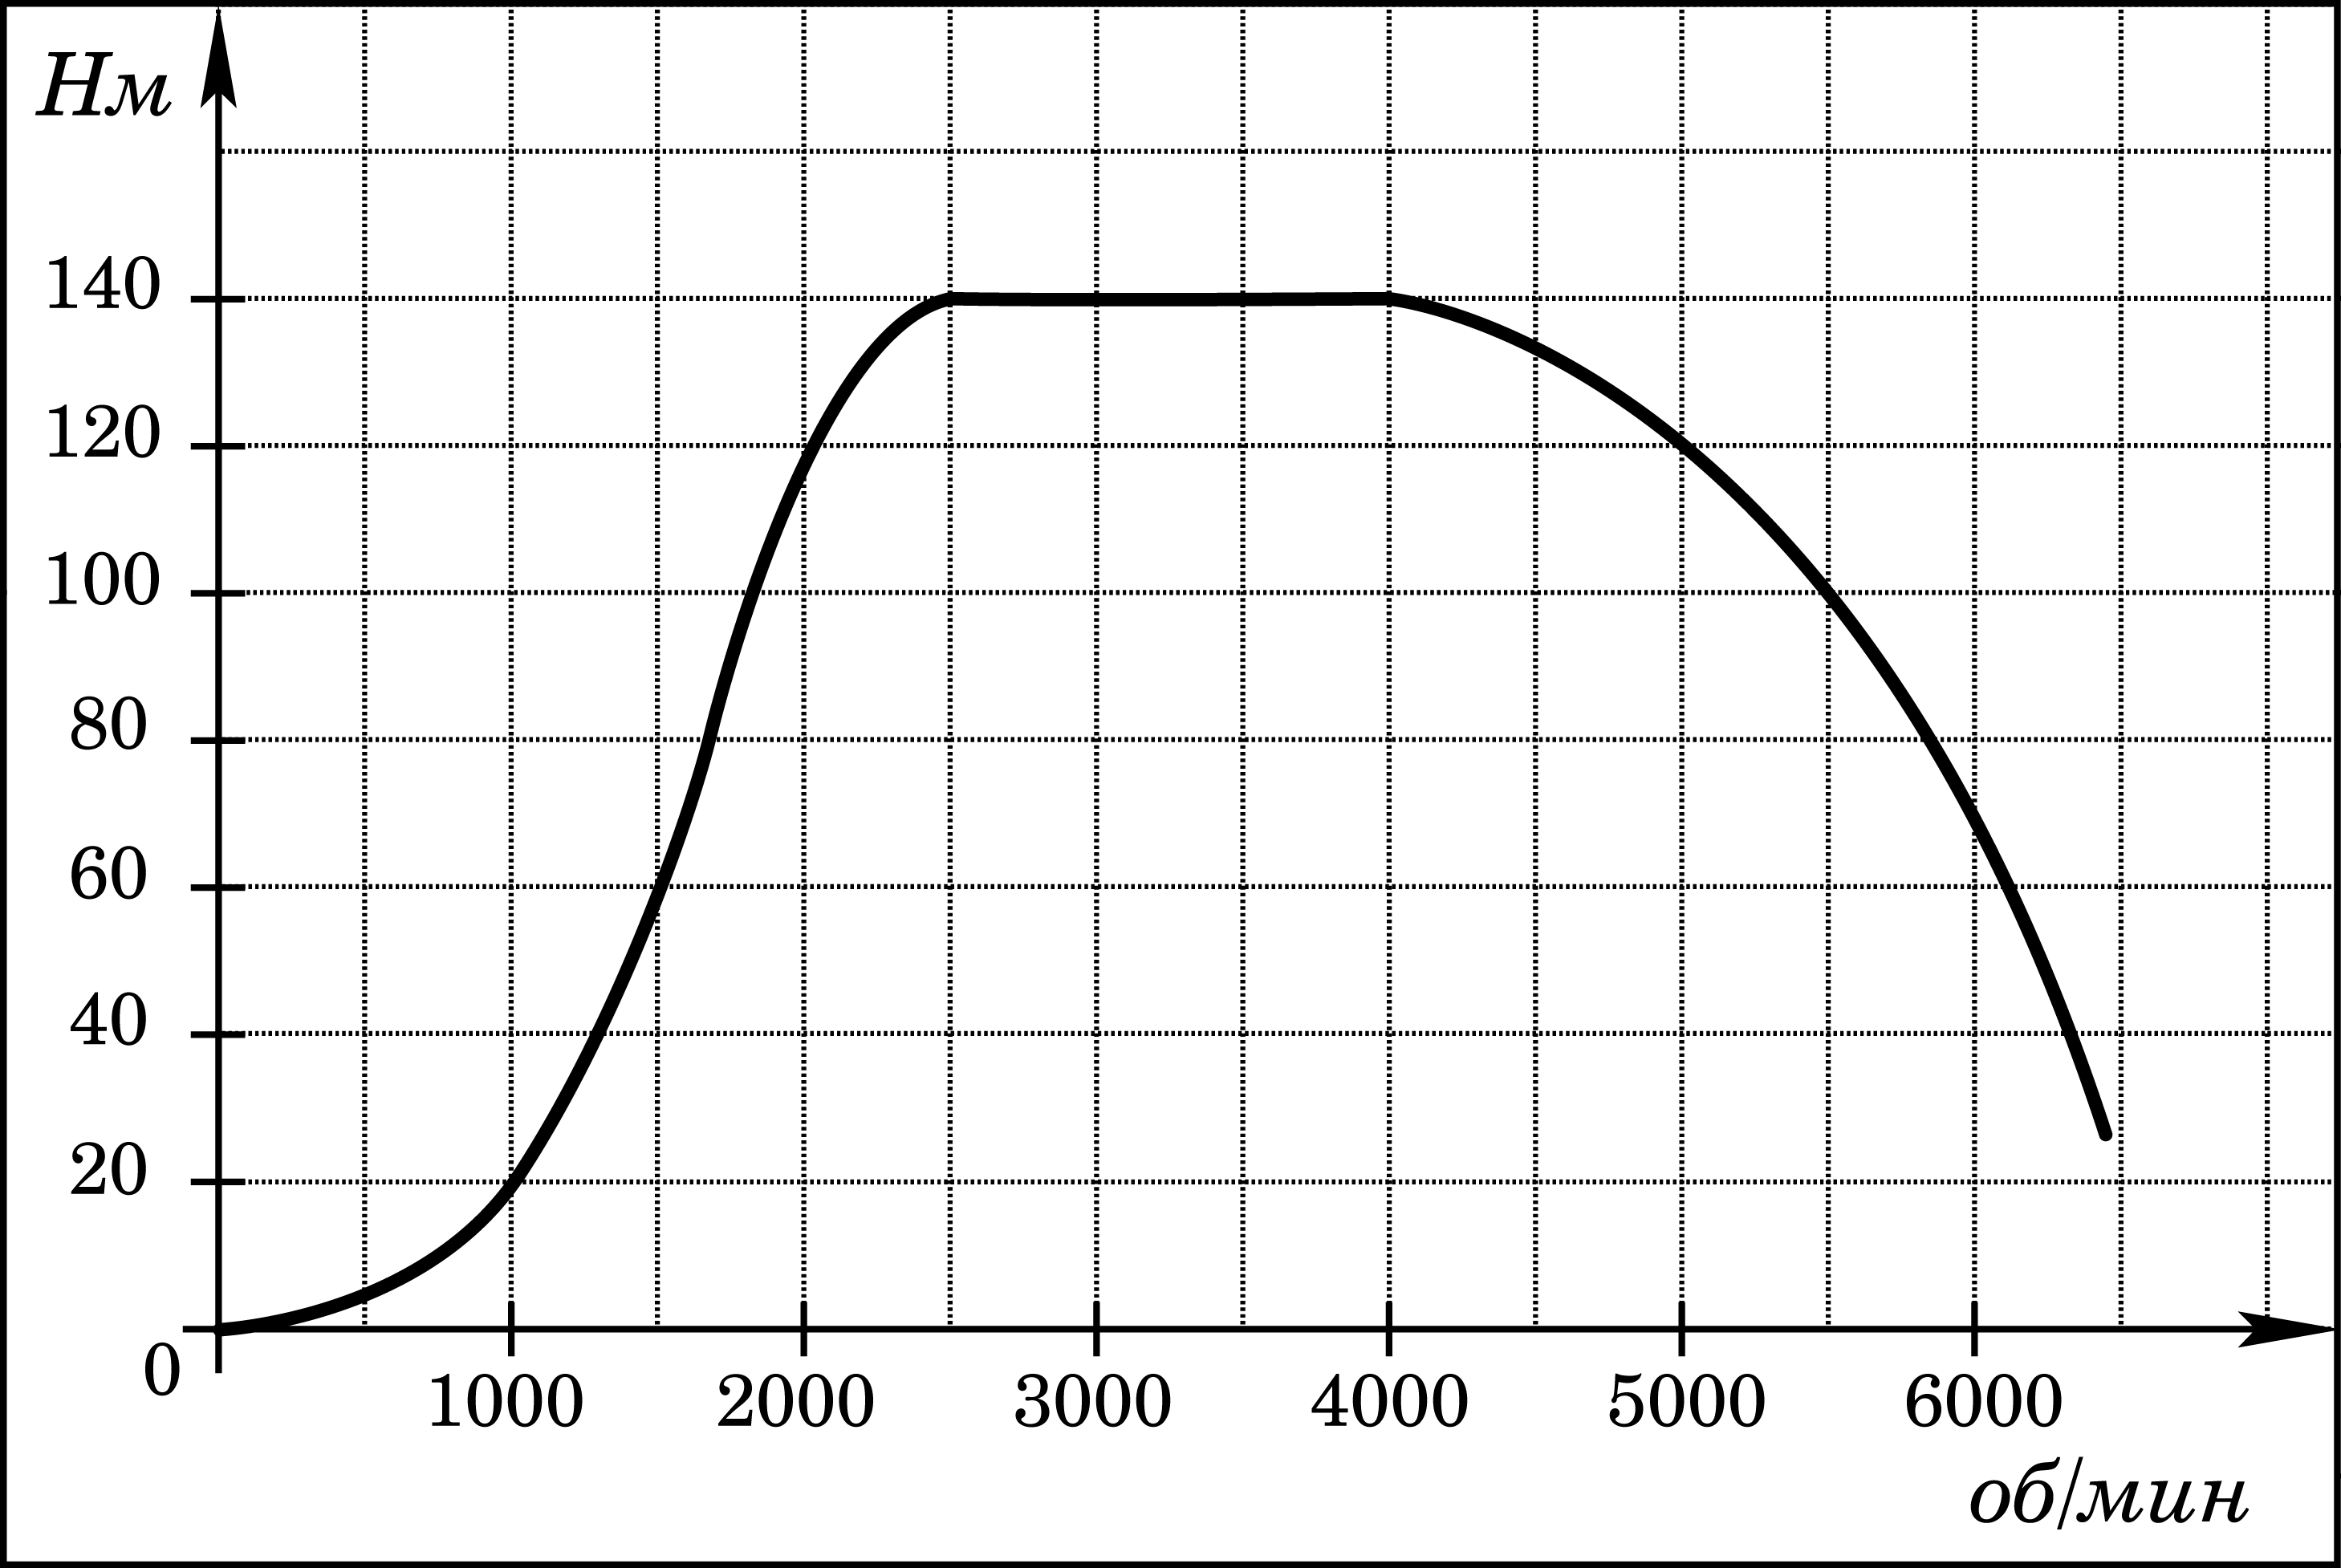
\includegraphics[scale=0.4]{26863.png}
 % innerimg0.png: 425x356 pixel, 72dpi, 14.99x12.56 cm, bb=0 0 425 356
\end{center}

\zad (� 26864)
�� ������� ���������� ����������� ��������� ������� �������������� ��������� �� ����� ��� �������� � ������. �� ��� ������� ������������� ����� �������� � ������. �� ��� ������� --- �������� ������ � �$\cdot$�. ����� ���������� ����� ��������, �������� ������ ������ ���� �� ����� 60 �$\cdot$�. ����� ���������� ����� �������� ��������� � ������ ����������, ����� ���������� ����� ��������?
\begin{center}
 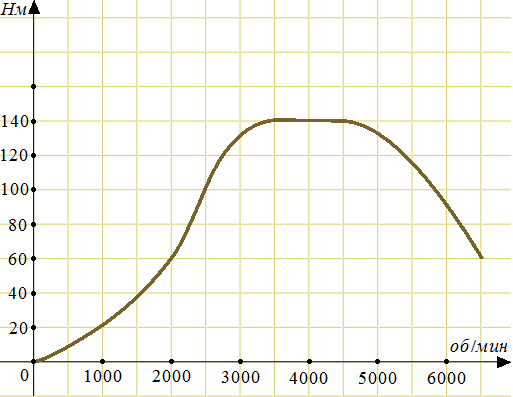
\includegraphics[scale=0.5]{26864.png}
 % innerimg0.png: 425x356 pixel, 72dpi, 14.99x12.56 cm, bb=0 0 425 356
\end{center}

\zad (� 26866)
�� ������� ������� ������� ��������� ��������� ��������� ����������. �� ��� ������� ������������� ����� � �������, ��������� �� ������� ���������, �� ��� ������� --- ����������� ��������� � �������� �������. ���������� �� �������, ������� ����� ��������� ���������� �� ����������� $60^{\circ}C$ �� ����������� $90^{\circ}C$.
\begin{center}
 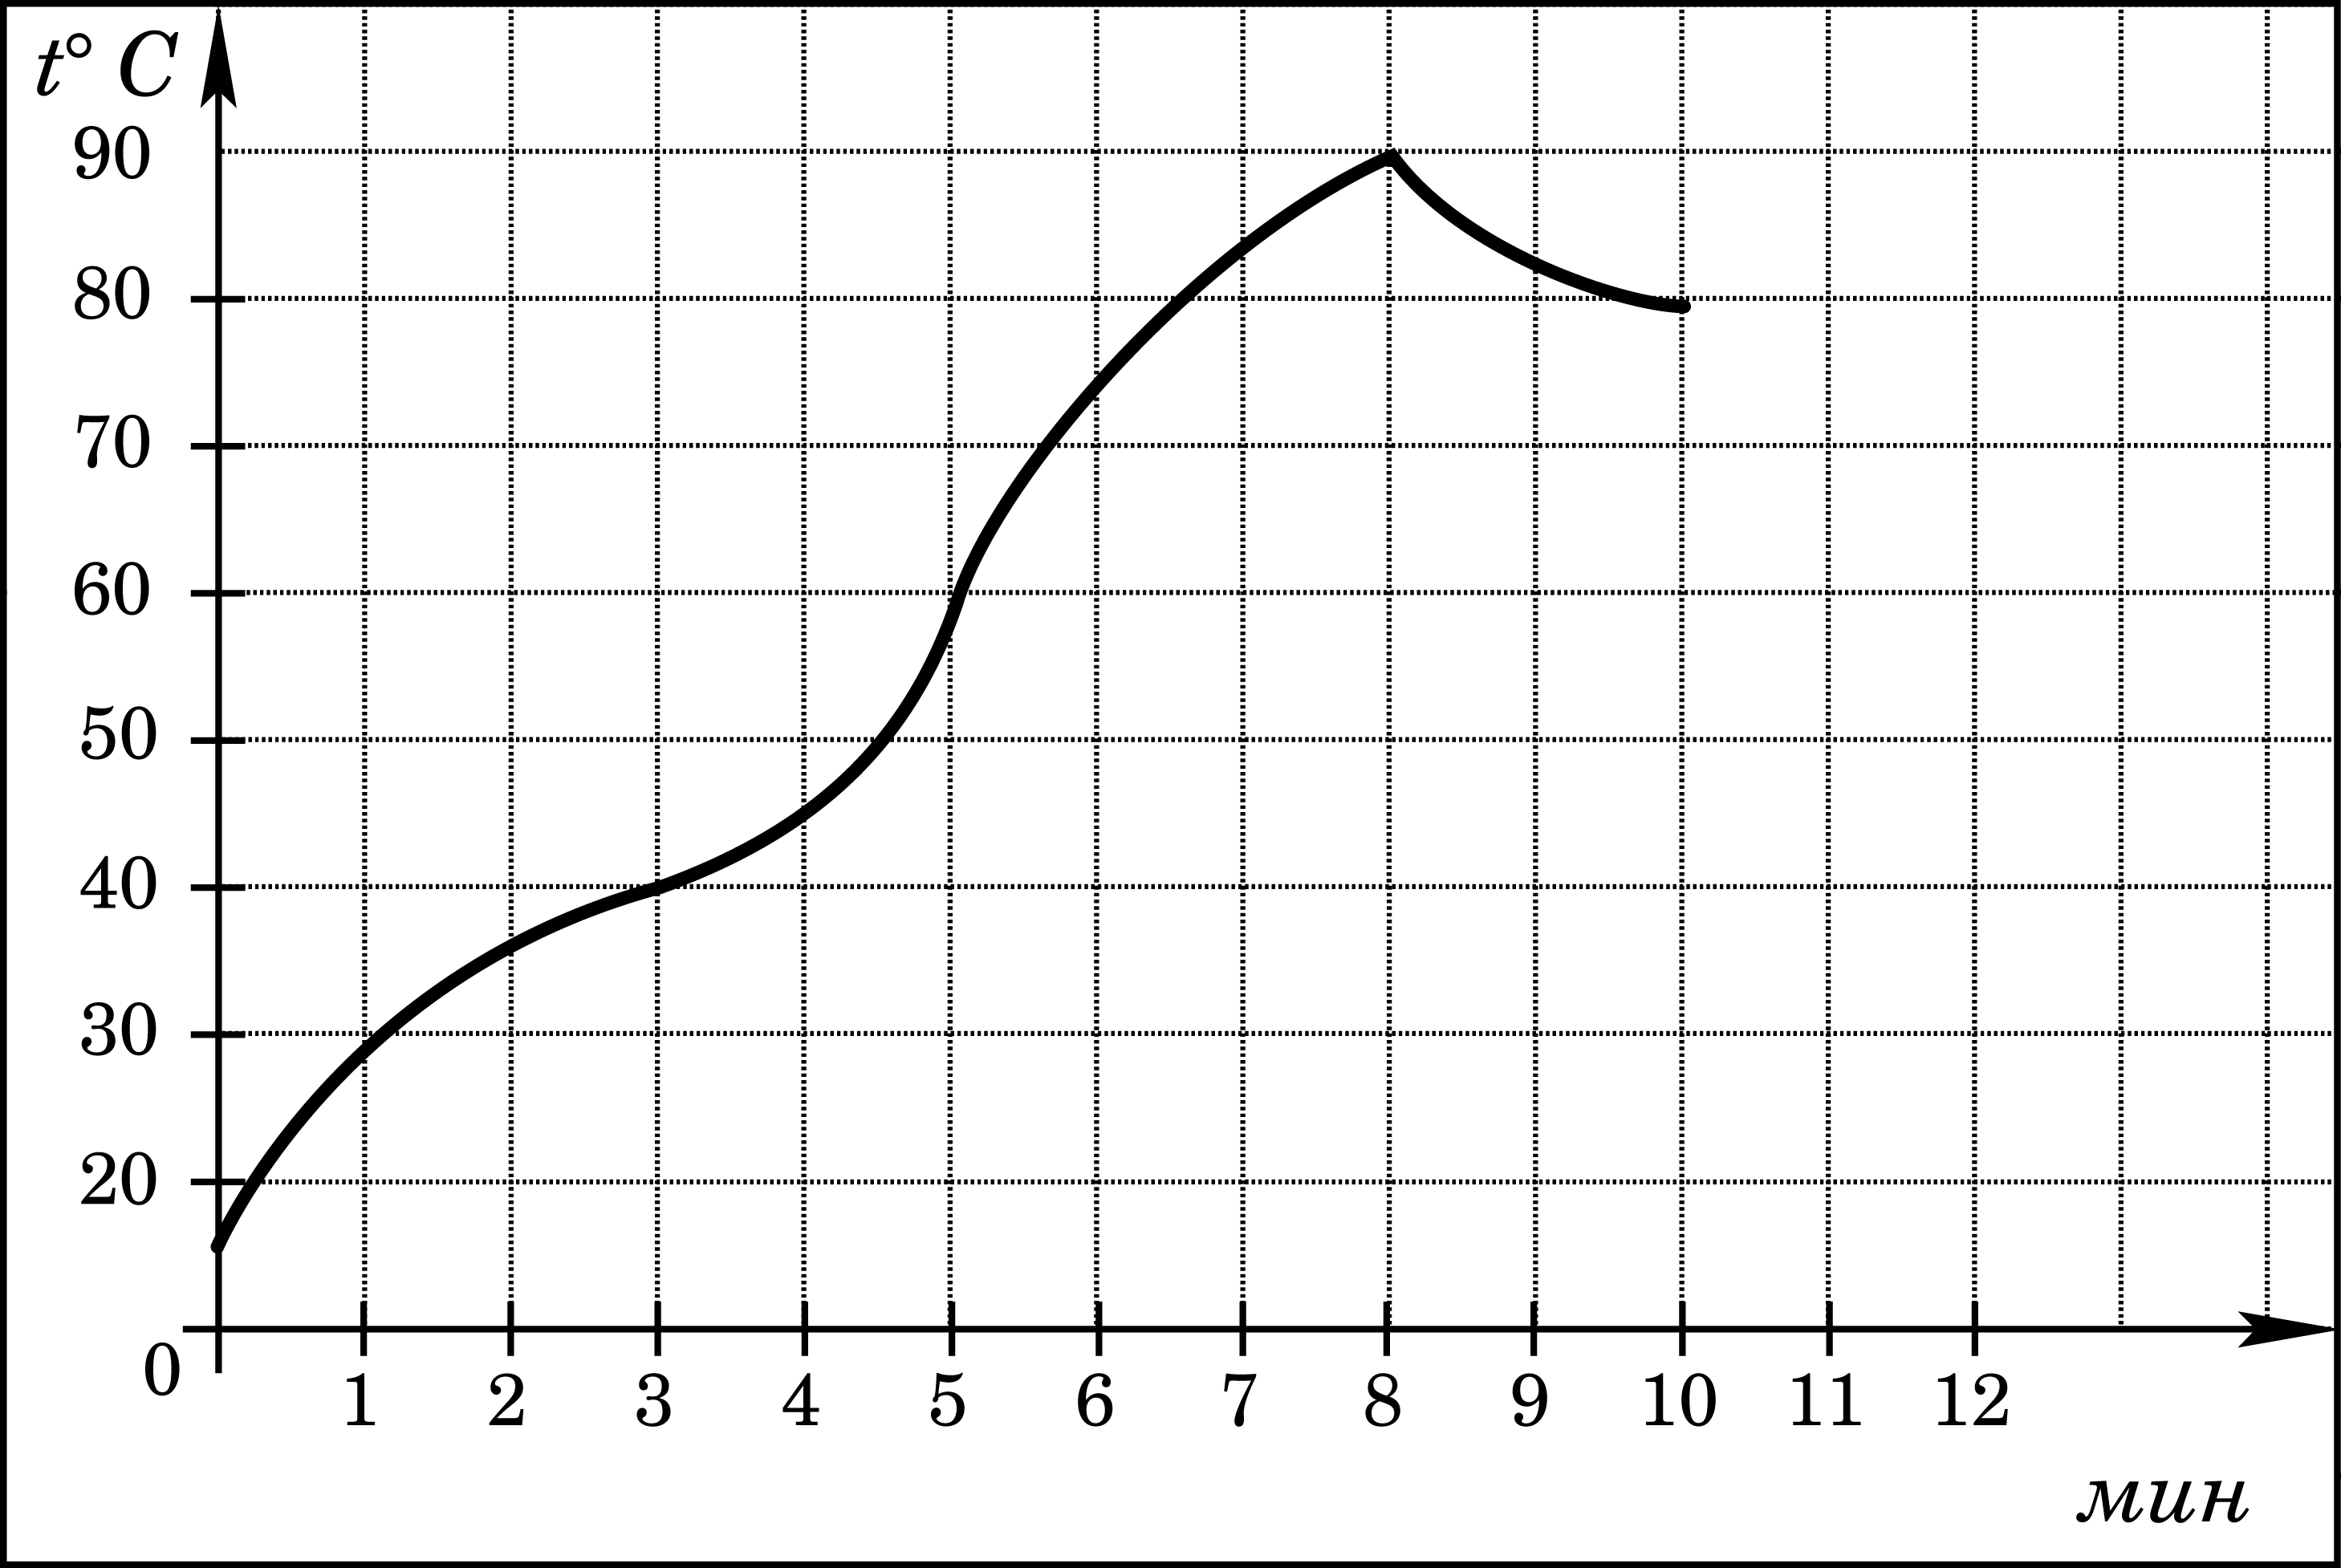
\includegraphics[scale=0.35]{26866.png}
 % innerimg0.png: 425x356 pixel, 72dpi, 14.99x12.56 cm, bb=0 0 425 356
\end{center}


\zad (� 26871)
�� ������� ������� ������� �������� �������� ���������� �������, ���������� � ������ � 3 �� 15 ������� 1909 ����. �� ����������� ����������� ����� ������, �� ��������� � ���������� �������, �������� � ��������������� ����, � �����������. ��� ����������� ������ ����� �� ������� ��������� ������. ���������� �� �������, ������ ����� ������� ������ 5 ����������� �������.
\begin{center}
 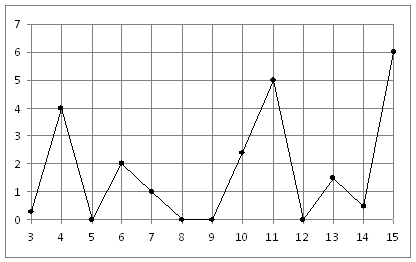
\includegraphics[scale=0.65]{26871.png}
 % innerimg0.png: 425x356 pixel, 72dpi, 14.99x12.56 cm, bb=0 0 425 356
\end{center}



\zad (� 26872)
�� ������� ������� ������� �������� ���� ����� �� ������ �������� �������� ������ �� ��� ������� ��� � 17 �� 31 ������� 2004 ����. �� ����������� ����������� ����� ������, �� ��������� � ���� ������� ����� � �������� ���. ��� ����������� ������ ����� �� ������� ��������� ������. ���������� �� ������� ���������� ���� ����� �� ������ �������� ������ � ��������� ������ (� �������� ��� �� �������).
\begin{center}
 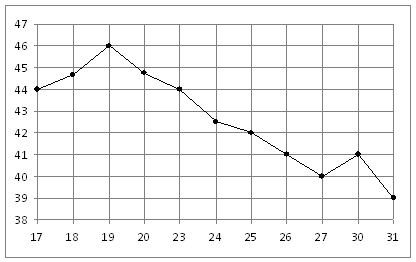
\includegraphics[scale=0.65]{26872.png}
 % innerimg0.png: 425x356 pixel, 72dpi, 14.99x12.56 cm, bb=0 0 425 356
\end{center}

\zad (� 26873)
�� ������� ������� ������� �������� ���� ������ �� ������ �������� �������� ������ �� ��� ������� ��� � 6 �� 20 ��� 2009 ����. �� ����������� ����������� ����� ������, �� ��������� � ���� ����� ������ � �������� ���. ��� ����������� ������ ����� �� ������� ��������� ������. ���������� �� ������� ���������� ���� ������ �� ������ �������� ������ � ��������� ������ (� �������� ��� �� �����).
\begin{center}
 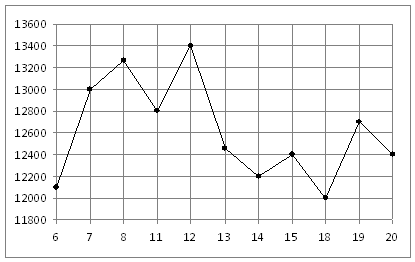
\includegraphics[scale=0.6]{26873.png}
 % innerimg0.png: 425x356 pixel, 72dpi, 14.99x12.56 cm, bb=0 0 425 356
\end{center}

\zad (� 27516)
�� ��������� �������� �������������� ����������� ������� � �����-���������� �� ������ ����� 1999 ����. �� ����������� ����������� ������, �� ��������� � ����������� � �������� �������. ���������� �� ��������� ���������� �������������� ����������� �� ������ �������� 1999 ����. ����� ����� � �������� �������.
\begin{center}
 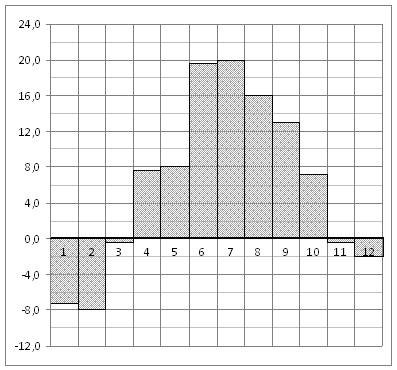
\includegraphics[scale=0.6]{27516.png}
 % innerimg0.png: 425x356 pixel, 72dpi, 14.99x12.56 cm, bb=0 0 425 356
\end{center}

\zad (� 263863)
����� ������� ��������� � �������������� ������, ��������� ����, ����������� �� ������, ������� ������ �� ��������. �� ������� ���������� ��� ����������� ��� ���������� ��������. �� ��� ������� ������������� �������� (� ���������� � ���), �� ��� ������� --- ���� (� ������ ����). ���������� �� �������, ���� ����� ��������� ���� (� ������ ����) ��� �������� 200 ��/�?
\begin{center}
 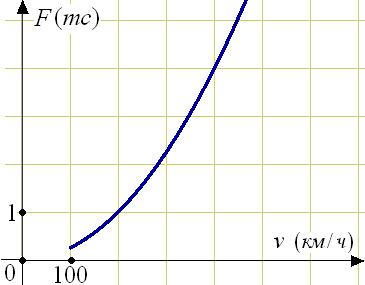
\includegraphics[scale=0.6]{263863.JPG}
 % innerimg0.png: 425x356 pixel, 72dpi, 14.99x12.56 cm, bb=0 0 425 356
\end{center}

\zad (� 263864)
� ��������� �������� ���������� ��������� � ��� ������ ������ �� �������������� �����. ��� �������������� ������������ ���������� ��������� ���������� ���� ��������� ����� ������������. �� ������� ���������� ����������� ��������� ����� �� ���� ������� ������������ � ��������� ��� ��������� ��������. �� ��� ������� ������������� ���� ������� � ��������, �� ��� ������� --- ���� ��������� �������������� ����� (� ����������� ����). ��� ����� ���� ������� ���� ��������� ��������� 150 ��$\cdot$�? ����� ����� � ��������.
\begin{center}
 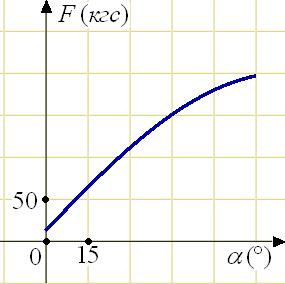
\includegraphics[scale=0.6]{263864.JPG}
 % innerimg0.png: 425x356 pixel, 72dpi, 14.99x12.56 cm, bb=0 0 425 356
\end{center}

\zad (� 263865)

� ���� ���������� ������� ���������� ��������� �������� (��������), ������� ��� �� �������� � �������, �� �������� ���������� �����������. �� ������� ��� ����������� ������������ ��������. �� ��� ������� ������������� ����� � �������, ��������� � ������� ������ �������, �� ��� ������� --- ����� ����������� ��������, ������� ��� �� ������� � ������� (� �������). ���������� �� �������, ������� ������� �������� �������� � ������� �� ��� ������?
\begin{center}
 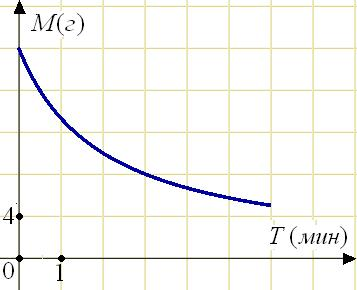
\includegraphics[scale=0.6]{263865.JPG}
 % innerimg0.png: 425x356 pixel, 72dpi, 14.99x12.56 cm, bb=0 0 425 356
\end{center}

\zad (� 263866)
�������� ��������� � ���������� ������������ �������������� ��������������, ������� ����� ������, ����������� �������� � ������ ������. ��� ���� �������� ���� ���� � ������������� ���� ���������������� --- ��� ������ �������������, ��� ������ ���� ���� � ��� ������� ��������� ����� ���������. �� ������� �������� ����������� ���� ���� �� �������� �������������. �� ��� ������� ������������� ������������� (� ����), �� ��� ������� --- ���� ���� � �������. ��� � ���� ���������������� ���������� � 8 �� 6 �����. �� ������� ���� ��� ���� ����������� ������������� ����?
\begin{center}
 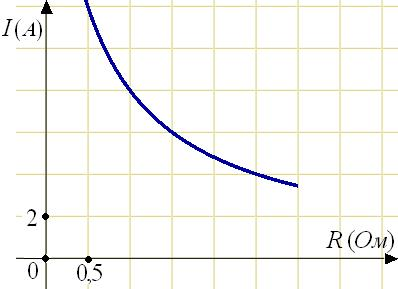
\includegraphics[scale=0.6]{263866.JPG}
 % innerimg0.png: 425x356 pixel, 72dpi, 14.99x12.56 cm, bb=0 0 425 356
\end{center}



\newpage
 \twocolumn[\section*{ ������� 3 ���2016.}] \setcounter{z}{0}

\zad (� 5085)
�� ��������� ������ � �������� �������� 1 �� $\times$  1 �� ��������� ����������� (��. �������). ������� ��� ������� � ���������� �����������.
\begin{center}
 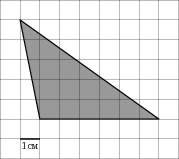
\includegraphics[scale=0.7]{5085.png}
 % 5085.png: 179x159 pixel, 72dpi, 6.32x5.61 cm, bb=0 0 179 159
\end{center}



\zad (� 5283)
�� ��������� ������ � �������� �������� 1 �� $\times$  1 �� ���������� �������� (��. �������). ������� �� ������� � ���������� �����������.
\begin{center}
 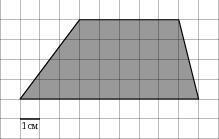
\includegraphics[scale=0.7]{5283.png}
 % 5283.png: 219x139 pixel, 72dpi, 7.73x4.90 cm, bb=0 0 219 139
\end{center}



\zad (� 21499)
������� ������� ���������������, ������������� �� �������.
\begin{center}
 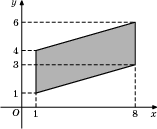
\includegraphics[scale=0.8]{21499.png}
 % 21499.png: 157x129 pixel, 72dpi, 5.54x4.55 cm, bb=0 0 157 129
\end{center}



\zad (� 21699)
������� ������� ���������������, ������� �������� ����� ���������� $(3;7)$, $(6;4)$, $(6;7)$, $(3;10)$.
\begin{center}
 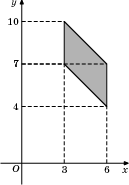
\includegraphics[scale=0.8]{21699.png}
 % 21699.png: 129x185 pixel, 72dpi, 4.55x6.53 cm, bb=0 0 129 185
\end{center}



\zad (� 21899)
������� ������� ������������, ������� �������� ����� ���������� $(1;7)$, $(5;7)$, $(3;9)$.
\begin{center}
 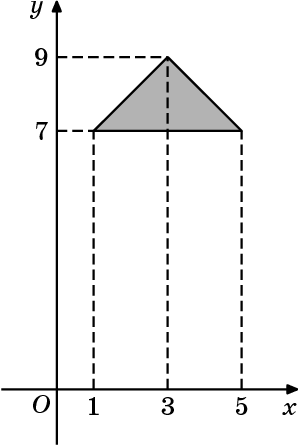
\includegraphics[scale=0.8]{21899.png}
 % 21899.png: 298x446 pixel, 188dpi, 4.03x6.03 cm, bb=0 0 114 171
\end{center}



\zad (� 22301)
������� ������� ������������, ������������� �� �������.
\begin{center}
 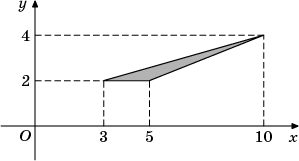
\includegraphics[scale=0.8]{22301.png}
 % 22301.png: 299x161 pixel, 116dpi, 6.54x3.52 cm, bb=0 0 185 100
\end{center}



\zad (� 22501)
������� ������� ��������, ������� ������� ����� ���������� $(1;1)$, $(10;1)$, $(6;7)$, $(2;7)$.
\begin{center}
 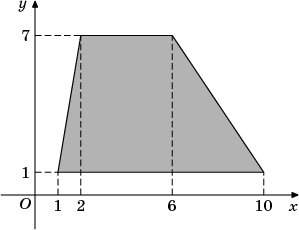
\includegraphics[scale=0.7]{22501.png}
 % 22501.png: 299x230 pixel, 116dpi, 6.54x5.03 cm, bb=0 0 185 143
\end{center}



\zad (� 24099)
������� ������� ��������, ������� ������� ����� ���������� $(4;3)$, $(10;3)$, $(6;9)$, $(1;9)$.
\begin{center}
 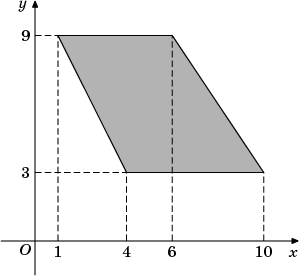
\includegraphics[scale=0.7]{24099.png}
 % 24099.png: 299x276 pixel, 116dpi, 6.54x6.04 cm, bb=0 0 185 171
\end{center}


\zad (� 5183)
�� ��������� ������ � �������� �������� 1 �� $\times$ 1 �� ��������� ����������� (��. �������). ������� ��� ������� � ���������� �����������.
\begin{center}
 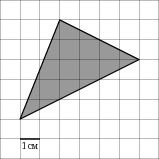
\includegraphics[scale=0.7]{5183.png}
 % 5183.png: 159x159 pixel, 72dpi, 5.61x5.61 cm, bb=0 0 159 159
\end{center}


\zad (� 5317)
�� ��������� ������ � �������� �������� 1 �� $\times$ 1 �� ���������� ������ (��. �������). ������� �� ������� � ���������� �����������.
\begin{center}
 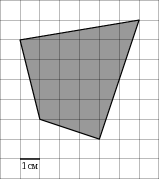
\includegraphics[scale=0.7]{5317.png}
 % 5317.png: 159x179 pixel, 72dpi, 5.61x6.32 cm, bb=0 0 159 179
\end{center}


\zad (� 24239)
������� ������� �����, ������������� �� �������.
\begin{center}
 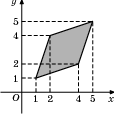
\includegraphics[scale=0.7]{24239.png}
 % 5085.png: 179x159 pixel, 72dpi, 6.32x5.61 cm, bb=0 0 179 159
\end{center}


\zad (� 24271)
������� ������� ����������� ������ �� ������������ ���������.
\begin{center}
 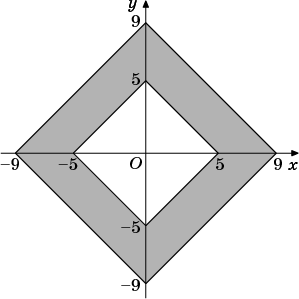
\includegraphics[scale=0.7]{24271.png}
 % 5085.png: 179x159 pixel, 72dpi, 6.32x5.61 cm, bb=0 0 179 159
\end{center}


\zad (� 24273)
������� ������� ����������� ������ �� ������������ ���������.
\begin{center}
 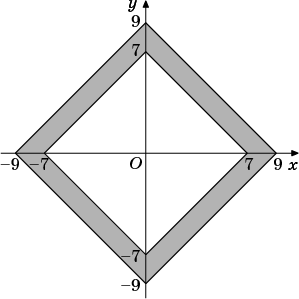
\includegraphics[scale=0.7]{24273.png}
 % 5085.png: 179x159 pixel, 72dpi, 6.32x5.61 cm, bb=0 0 179 159
\end{center}

\zad (� 248301)
������� ������� ������������, ������������� �� ��������� ������ � �������� ������ 1 �� $\times$  1 �� (��. ���.). ����� ����� � ���������� �����������.
\begin{center}
 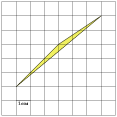
\includegraphics[scale=0.7]{248301.png}
 % 5085.png: 179x159 pixel, 72dpi, 6.32x5.61 cm, bb=0 0 179 159
\end{center}



\zad (� 252335)
������� ������� ������������, ������������� �� ��������� ������ � �������� ������ 1 �� $\times$ 1 �� (��. ���.). ����� ����� � ���������� �����������.
\begin{center}
 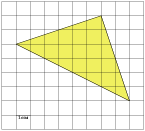
\includegraphics[scale=0.7]{252335.png}
 % 5085.png: 179x159 pixel, 72dpi, 6.32x5.61 cm, bb=0 0 179 159
\end{center}



\zad (� 252345)
������� ������� ������������, ������������� �� ��������� ������ � �������� ������ 1 �� $\times$ 1 �� (��. ���.). ����� ����� � ���������� �����������.
\begin{center}
 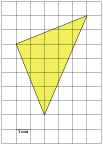
\includegraphics[scale=0.7]{252345.png}
 % 5085.png: 179x159 pixel, 72dpi, 6.32x5.61 cm, bb=0 0 179 159
\end{center}



\zad (� 252347)
������� ������� ������������, ������������� �� ��������� ������ � �������� ������ 1 �� $\times$ 1 �� (��. ���.). ����� ����� � ���������� �����������.
\begin{center}
 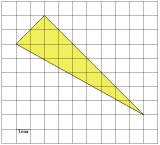
\includegraphics[scale=0.7]{252347.png}
 % 5085.png: 179x159 pixel, 72dpi, 6.32x5.61 cm, bb=0 0 179 159
\end{center}



\zad (� 256455)
������� ������� ����������������, ������������� �� ��������� ������ � �������� ������ 1 �� $\times$ 1 �� (��. ���.). ����� ����� � ���������� �����������.
\begin{center}
 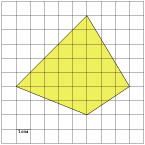
\includegraphics[scale=0.7]{256455.png}
 % 5085.png: 179x159 pixel, 72dpi, 6.32x5.61 cm, bb=0 0 179 159
\end{center}



\zad (� 258595)
������� ������� ����������������, ������������� �� ��������� ������ � �������� ������ 1 �� $\times$  1 �� (��. ���.). ����� ����� � ���������� �����������.
\begin{center}
 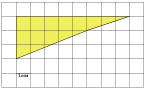
\includegraphics[scale=0.7]{258595.png}
 % 5085.png: 179x159 pixel, 72dpi, 6.32x5.61 cm, bb=0 0 179 159
\end{center}



\zad (� 263375)
������� ������� ����������������, ������������� �� ��������� ������ � �������� ������ 1 �� $\times$ 1 �� (��. ���.). ����� ����� � ���������� �����������.
\begin{center}
 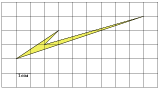
\includegraphics[scale=0.7]{263375.png}
 % 5085.png: 179x159 pixel, 72dpi, 6.32x5.61 cm, bb=0 0 179 159
\end{center}



\zad (� 263415)
������� ������� ����������������, ������������� �� ��������� ������ � �������� ������ 1 �� $\times$ 1 �� (��. ���.). ����� ����� � ���������� �����������.
\begin{center}
 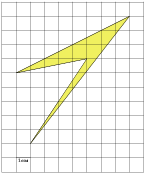
\includegraphics[scale=0.7]{263415.png}
 % 5085.png: 179x159 pixel, 72dpi, 6.32x5.61 cm, bb=0 0 179 159
\end{center}



\zad (� 263417)
������� ������� ����������������, ������������� �� ��������� ������ � �������� ������ 1 �� $\times$ 1 �� (��. ���.). ����� ����� � ���������� �����������.
\begin{center}
 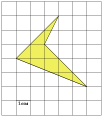
\includegraphics[scale=0.7]{263417.png}
 % 5085.png: 179x159 pixel, 72dpi, 6.32x5.61 cm, bb=0 0 179 159
\end{center}



\zad (� 263475)
������� (� ��$^2$) ������� $S$ ������, ������������ �� ��������� ������ � �������� ������ 1 �� $\times$ 1 �� (��. ���.). � ������ �������� $\dfrac{S}{\pi}$.
\begin{center}
 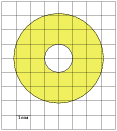
\includegraphics[scale=0.7]{263475.png}
 % 5085.png: 179x159 pixel, 72dpi, 6.32x5.61 cm, bb=0 0 179 159
\end{center}



\zad (� 263479)
������� (� ��$^2$) ������� $S$ ������, ������������ �� ��������� ������ � �������� ������ 1 �� $\times$ 1 �� (��. ���.). � ������ �������� $\dfrac{S}{\pi}$.
\begin{center}
 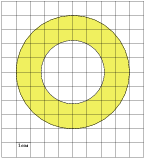
\includegraphics[scale=0.7]{263479.png}
 % 5085.png: 179x159 pixel, 72dpi, 6.32x5.61 cm, bb=0 0 179 159
\end{center}


\zad (� 315137)
�� ��������� ������ ��������� ���� �������� 30. ������� ������� ��������������� �������.
\begin{center}
 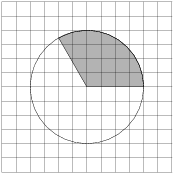
\includegraphics[scale=0.6]{315137.png}
 % 21499.png: 157x129 pixel, 72dpi, 5.54x4.55 cm, bb=0 0 157 129
\end{center}


\zad (� 322637)
�� ��������� ������ ���������� ��� �����. ������� ����������� ����� ����� 2. ������� ������� �������������� ������.
\begin{center}
 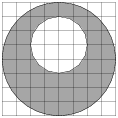
\includegraphics[scale=0.8]{322637.png}
 % 21499.png: 157x129 pixel, 72dpi, 5.54x4.55 cm, bb=0 0 157 129
\end{center}


\zad (� 322735)
�� ��������� ������ ���������� ��� �����. ������� ����������� ����� ����� 1. ������� ������� �������������� ������.
\begin{center}
 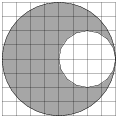
\includegraphics[scale=0.7]{322735.png}
 % 21499.png: 157x129 pixel, 72dpi, 5.54x4.55 cm, bb=0 0 157 129
\end{center}



\zad (� 322737)
�� ��������� ������ ���������� ��� �����. ������� ����������� ����� ����� 16. ������� ������� �������������� ������.
\begin{center}
 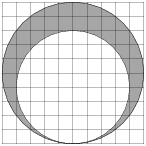
\includegraphics[scale=0.6]{322737.png}
 % 21499.png: 157x129 pixel, 72dpi, 5.54x4.55 cm, bb=0 0 157 129
\end{center}



\zad (� 322825)
�� ��������� ������ �������� ����. ������ ������� �����, ���� ������� ��������������� ������� ����� 33?
\begin{center}
 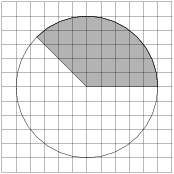
\includegraphics[scale=0.6]{322825.png}
 % 21499.png: 157x129 pixel, 72dpi, 5.54x4.55 cm, bb=0 0 157 129
\end{center}



\zad (� 322829)
�� ��������� ������ �������� ����. ������ ������� �����, ���� ������� ��������������� ������� ����� 60?
\begin{center}
 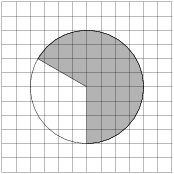
\includegraphics[scale=0.7]{322829.png}
 % 21499.png: 157x129 pixel, 72dpi, 5.54x4.55 cm, bb=0 0 157 129
\end{center}




\zad (� 317343)
� ������������ $ABC$ $DE$ --- ������� �����. ������� ������������ $ADE$ ����� 5. ������� ������� ������������ $ABC$.

\zad (� 317447)
������� ��������������� $ABCD$ ����� 30. ����� $E$ --- �������� ������� $CD$. ������� ������� �������� $ABED$.

\zad (� 319065)
������� ���������������  $ABCD$ ����� 164. ������� ������� ���������������  $A'B'C'D'$, ��������� �������� �������� �������� ������ ������� ���������������.

\zad (� 319161)
������� ���������������  $ABCD$ ����� 36. �����  $E$ --- �������� ������� $CD$. ������� ������� ������������ $ADE$.

\zad (� 319255)
������� ������������ $ABC$ ����� 12. $DE$ --- ������� �����, ������������ ������� $AB$. ������� ������� �������� $ABDE$.









%
%
%\zad (� 55019)
%������� ������� �����, ���� ��� ������� ����� 49, � ���� �� ����� ����� $150^{\circ}$.
%
%\zad (� 56017)
%�������� �������������� ����� 52, � ������� ����� 25,5. ������� ��������� ����� ��������������.
%
%\zad (� 56619)
%���� ��� �������, �������������� ��������� ��������������� ������������, ����� $30^{\circ}$. ������� ������� ������� ������������, ���� ��� ������� ����� 729.

\zad (� 56817)
�������� ������������ ����� 20, � ������ ��������� ���������� ����� 2. ������� ������� ����� ������������.

\zad (� 57017)
������ �������� ����� 11, ������� ����� 143. ������� ������� ����� ��������.

%\zad (� 57217)
%��������� ������������� �������� ����� 6 � 18. �� ������� ����� 144. ������� ������ ���� ���� ��������. ����� ����� � ��������.

\zad (� 57417)
����� ����������, ������ ������� ����� 3, ������ �������������, �������� �������� ����� 62. ������� ��� �������.

\zad (� 57617)
������� ������� ����� ������� 46 ����� 207. ������� ����� ��� ����.

%\zad (� 57817)
%������� ���������� �� ����� $A(-1;4)$  �� ��� �������.
%
%\zad (� 58017)
%������� �������� �����, ������������ ����� $A(-6;4)$  ������������ ������ ���������.
%
%\zad (� 58217)
%������� �������� �������� �������, ������������ ����� $A(-1;5)$  � $B(5;2)$.
%
%\zad (� 58417)
%������� ����� �������, ������������ ����� $A(4;-6)$  � $B(-4;9)$.
%
%\zad (� 58617)
%������� ������� ����������� ������, ���������� ����� ����� � ������������ $(-1;0)$ � $(0;7)$.
%
%\zad (� 58817)
%������� �������� ����� ����������� ��� $Oy$ � ������, ���������� ����� ����� $B(2;12)$ � ������������ ������, ���������� ����� ������ ��������� � ����� $A(2;39)$.
%
%\zad (� 59017)
%����� $O(0;0)$, $A(7;12)$, $B(9;15)$, $C(2;3)$  �������� ��������� ����������������. ������� �������� ����� $P$ ����������� ��� ����������.
%
%\zad (� 59217)
%������� �������� ����� ����������� ������, �������� ���������� ${6x+17y=8,5}$, � ���� $Oy$.
%
%\zad (� 59417)
%���������� � ������� � ������ ��������� �������� ����� ����� $P(-12;-5)$. ������� �� ������.
%
%\zad (� 59617)
%������� �������� ������ ����������, ��������� ����� �������������� $ABCD$, ������� �������� ����� ���������� ��������������
% $(7;12)$, $(7;4)$, $(1;4)$, $(1;12)$.
%
%\zad (� 59817)
%������� �������� ������ ����������, ��������� ����� ������������, ������� �������� ����� ����������
% $(10;0)$, $(0;-24)$, $(10;-24)$.
%
%\zad (� 60017)
%������� ������� ������������, ������� �������� ����� ����������
% $(2;13)$, $(17;15)$, $(17;21)$.
%
%\zad (� 60217)
%��� ������� �������������� $ABCD$ ����� 12 � 5. ������� ����� ����� ��������
%$\overrightarrow{AB}$  � $\overrightarrow{AD}$.
%
%\zad (� 60417)
%��� ������� �������������� $ABCD$ ����� 8 � 68.
% ��������� ������������ � ����� $O$.������� ����� �������� �������� $\overrightarrow{AO}$
% � $\overrightarrow{BO}$.
%\begin{center}
% 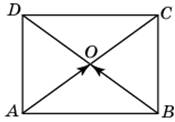
\includegraphics[scale=0.7]{60417.jpg}
% % 60417.jpg: 175x122 pixel, 96dpi, 4.63x3.23 cm, bb=0 0 131 92
%\end{center}
%
%
%
%\zad (� 60617)
%��������� ����� $ABCD$ ����� 60 � 63. ������� ����� ������� $\overrightarrow{AB}-\overrightarrow{AC}$.
%
%\zad (� 60817)
%������� ����������� ������������ $ABC$ ����� $14\sqrt{3}$. ������� ����� ������� $\overrightarrow{AB}+\overrightarrow{AC}$.
%\begin{center}
% 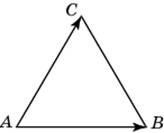
\includegraphics[scale=0.7]{60817.jpg}
% % 60817.jpg: 164x133 pixel, 96dpi, 4.34x3.52 cm, bb=0 0 123 100
%\end{center}
%
%
%
%\zad (� 61017)
%������ $\overrightarrow{AB}$  � ������� � ����� $A(11;4)$ ����� ���������� $\{6;6\}$.
% ������� �������� ����� $B$.
%
%\zad (� 61217)
%������ $\overrightarrow{AB}$ � ������ � ����� $B(7;-3)$ ����� ���������� $\{4;-13\}$.
%������� ����� ��������� ����� $A$.
%
%\zad (� 61417)
%��������� �������� ����� 17 � 27, ������� �������, ������ 16, �������� � ����� �� ��������� �������� ���� $150^{\circ}$. ������� ������� ��������.
%
%
%
%\zad (� 23931)
%������� ������� ������������� ��������, ������� ������� ����� ���������� $(4;1),$ $(10;1),$ $(6;9),$ $(4;9).$
%% \begin{center}
%%  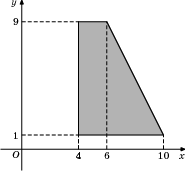
\includegraphics[scale=0.7]{23931.png}
%%  % 23931.png: 185x171 pixel, 72dpi, 6.53x6.03 cm, bb=0 0 185 171
%% \end{center}
%%
%%
%% \zad (� 56453)
%% ������� ����� ����� 18. ���� �� ��� ���������� � 4 ���� ������ ������. ������� ������� ���������.
%
% \zad (� 61251)
% ������ $\overrightarrow{AB}$ � ������ � ����� $B(1; -3)$ ����� ���������� $(4; 16)$. ������� ����� ��������� ����� $A$.
%
%
%\zad (� 54807)
%������� ������� ��������, ���� ��� ��������� ����� 20.
%
%\zad (� 54999)
%������� ������� ���������������, ���� ��� ��� ������� ����� 15 � 11, � ���� ����� ���� ����� $30^{\circ}$.
%
%\zad (� 55005)
%������� ������� �����, ���� ��� ������� ����� 27, � ���� �� ����� ����� $150^{\circ}$.
%
%\zad (� 55601)
%������� ����� ����� $\dfrac{132,25}{\pi}$. ������� ����� ��� ����������.
%
%\zad (� 55603)
%������� ����� ����� $\dfrac{441}{\pi}$. ������� ����� ��� ����������.
%
%\zad (� 55607)
%������� ������� ������� ����� ������� $\dfrac{19}{\sqrt{\pi}}$, ����������� ���� �������� ����� $90^{\circ}$.
%
%%\zad (� 55629)
%%������� ������� ������� ����� ������� $\dfrac{34}{\sqrt{\pi}}$, ����������� ���� �������� �����  $90^{\circ}$.
%
%\zad (� 55829)
%������� ������� ��������������, ���� ��� �������� ����� 68, � ��������� �������� ������ ����� $3:14$.
%
%%\zad (� 55835)
%%
%%������� ������� ��������������, ���� ��� �������� ����� 44, � ��������� �������� ������ ����� $3:8$.
%
%\zad (� 56029)
%�������� �������������� ����� 16, � ������� ����� 7,5. ������� ��������� ����� ��������������.
%
%%\zad (� 56033)
%%�������� �������������� ����� 48, � ������� ����� 23,5. ������� ��������� ����� ��������������.
%
%\zad (� 56229)
%������� ��������������� ����� 290, ��� ��� ������� ����� 20 � 110. ������� ������� ������ ����� ���������������.
%
%%\zad (� 56233)
%%������� ��������������� ����� 96, ��� ��� ������� ����� 32 � 64. ������� ������� ������ ����� ���������������.
%
%\zad (� 56329)
%������� ������� �����, ���� ��� ��������� ����� 36 � 4.
%
%%\zad (� 56335)
%%������� ������� �����, ���� ��� ��������� ����� 20 � 6.
%
%\zad (� 56529)
%������� �������������� ������������ ����� 90. ���� �� ��� ������� �� 3 ������ �������. ������� ������� �����.
%
%%\zad (� 56535)
%%������� �������������� ������������ ����� 135. ���� �� ��� ������� �� 3 ������ �������. ������� ������� �����.
%
%%\zad (� 56609)
%%���� ��� �������, �������������� ��������� ��������������� ������������, ����� $30^{\circ}$. ������� ������� ������� ������������, ���� ��� ������� ����� 1.
%
%\zad (� 56617)
%
%���� ��� �������, �������������� ��������� ��������������� ������������, ����� $30^{\circ}$. ������� ������� ������� ������������, ���� ��� ������� ����� 49.
%
%%\zad (� 56809)
%%�������� ������������ ����� 12, � ������ ��������� ���������� ����� 1. ������� ������� ����� ������������.
%
%\zad (� 56815)
%�������� ������������ ����� 88, � ������ ��������� ���������� ����� 10. ������� ������� ����� ������������.
%
%\zad (� 57009)
%������ �������� ����� 6, ������� ����� 18. ������� ������� ����� ��������.
%
%%\zad (� 57015)
%%������ �������� ����� 17, ������� ����� 153. ������� ������� ����� ��������.
%
%\zad (� 57209)
%��������� ������������� �������� ����� 13 � 17. �� ������� ����� 60. ������� ������ ���� ���� ��������. ����� ����� � ��������.
%
%%\zad (� 57217)
%%��������� ������������� �������� ����� 6 � 18. �� ������� ����� 144. ������� ������ ���� ���� ��������. ����� ����� � ��������.
%
%\zad (� 57409)
%����� ����������, ������ ������� ����� 2, ������ �������������, �������� �������� ����� 29. ������� ��� �������.
%
%%\zad (� 57411)
%%����� ����������, ������ ������� ����� 4, ������ �������������, �������� �������� ����� 63. ������� ��� �������.

\zad (� 57609)
������� ������� ����� ������� 3 ����� 15. ������� ����� ��� ����.
%
%%\zad (� 57613)
%%������� ������� ����� ������� 42 ����� 147. ������� ����� ��� ����.
%
%%\zad (� 57809)
%%������� ���������� �� ����� $A$ � ������������ $(-2;10)$ �� ��� �������.
%%
%%\zad (� 58063)
%%������� �������� �����, ������������ ����� $A(2;-12)$  ������������ ������ ���������.
%
%%\zad (� 58259)
%%������� �������� �������� �������, ������������ ����� $A(-1;2)$  � $B(2;2)$.
%
%\zad (� 58267)
%������� �������� �������� �������, ������������ ����� $A(1;-3)$  � $B(3;2)$.
%
%%\zad (� 58499)
%%������� ����� ������� $\overrightarrow{a}(-8;-6)$.
%
%%\zad (� 58501)
%%������� ����� ������� $\overrightarrow{a}(-12;5)$.
%
%\zad (� 58505)
%������� ����� ���� ������� �������, ������������ ����� $O(0;0)$ � $A(-24;-7)$, � ���� �������.
%
%%\zad (� 58507)
%%������� ����� ���� ������� �������, ������������ ����� $O(0;0)$ � $A(8;-6)$, � ���� �������.
%
%%\zad (� 58699)
%%������� ������� ����������� ������, ���������� ����� ����� � ������������ $(1;0)$ � $(0;16)$.
%
%\zad (� 58701)
%������� ������� ����������� ������, ���������� ����� ����� � ������������ $(2;0)$ � $(0;5)$.
%
%%\zad (� 58705)
%%������ $a$ �������� ����� ����� � ������������ $(0;10)$ � $(1;0)$. ������ $b$ �������� ����� ����� � ������������ $(0;20)$ � ����������� ������ $a$. ������� �������� ����� ����������� ������ $b$ � ���� $Ox$.
%
%%\zad (� 58707)
%%������ $a$ �������� ����� ����� � ������������ $(0;9)$ � $(2;0)$. ������ $b$ �������� ����� ����� � ������������ $(0;27)$ � ����������� ������ $a$. ������� �������� ����� ����������� ������ $b$ � ���� $Ox$.
%
%\zad (� 58901)
%����� $O(0;0)$, $A(2;-13)$, $B(2;14)$, $C(0;27)$ �������� ��������� ����������������. ������� �������� ����� $P$ ����������� ��� ����������.
%
%%\zad (� 58907)
%%����� $O(0;0)$, $A(2;17)$, $B(2;14)$, $C(0;-3)$  �������� ��������� ����������������. ������� �������� ����� $P$ ����������� ��� ����������.
%
%\zad (� 59299)
%������� �������� ����� ����������� ������, �������� ����������� $23x-24y=-4$ � $y=x$.
%
%%\zad (� 59303)
%%������� �������� ����� ����������� ������, �������� ����������� $23x+19y=-126$ � $y=x$.
%
%%\zad (� 59541)
%%������ ������� ������ ���� ���������� � ������� � ����� $P(6;8)$, ����� ��� �������� ��� �������?
%
%\zad (� 59943)
%������� ������� ����������������, ������� �������� ����� ���������� $(5;0)$, $(14;15)$, $(9;18)$, $(0;3)$.
%
%%\zad (� 59947)
%%������� ������� ����������������, ������� �������� ����� ���������� $(3;0)$, $(6;9)$, $(3;10)$, $(0;1)$.
%
%%\zad (� 60339)
%%��� ������� �������������� $ABCD$ ����� 96 � 180. ������� ��������� ������������ �������� $\overrightarrow{AB}$ � $\overrightarrow{AD}$.
%
%%\zad (� 60345)
%%��� ������� �������������� $ABCD$ ����� 3 � 4. ������� ��������� ������������ �������� $\overrightarrow{AB}$ � $\overrightarrow{AD}$.
%
%\zad (� 61363)
%��������� �������������� �������� ����� 15 � 25, � �� ������� ������� ����� 13. ������� ������� ��������.
%
%%\zad (� 61369)
%%��������� �������������� �������� ����� 4 � 10, � �� ������� ������� ����� 5. ������� ������� ��������.
%
%

\newpage \large
 \onecolumn
\section*{������� 4 ���2016.}
\setcounter{z}{0}

\zad (� 320843)
�� ���������� �������� 10 ����, �� 0 �� 9. ������ ����������� ����, ��� �������� ������� ����� ����� ������ 4?

\zad (� 320857)
�� ��������� ����������� ����� �� 40 �� 54 ������� �������� ���� �����. ������ ����������� ����, ��� ��� ������� �� 5?

\zad (� 321009)
� ������ �������� 10 �������. � ������� ������ ��� �������� ������ �������, ������� ������ ���� � ���� � ������� �� ����������. ������ ����������� ����, ��� ������ �., �������� � ������ ������, ����� � �������?

\zad (� 321209)
� ��������� ������ �� 3000 ����������� �� ���� ��������� 1520 ���������. ������� ������� �������� ������� � ���� ������. ��������� ��������� �� ��������.

\zad (� 321045)
��������� ����� ������� ������. ������� ������������ ������� ����� ���������������� �������
� = \{����� ����� ����� 9\}?

\zad (� 283451)
� ��������� ������������ ������� ��� ��������� �����. ������� ����������� ����, ��� � ����� ������� 6 �����. ��������� ��������� �� �����.

\zad (� 283449)
� ��������� ������������ ������� ��� ��������� �����. ������� ����������� ����, ��� � ����� ������� 15 �����. ��������� ��������� �� �����.

\zad (� 283475)
� ��������� ������������ ������������ ������ ������� ������. ������� ����������� ����, ��� ���� ������� ����� ���� ���.

% \zad (� 283471)
% � ��������� ������������ ������������ ������ ������� ���������. ������� ����������� ����, ��� ���� �� ������� �� ����.

\zad (� 322283)
����� ������� ������������� ����� �������� ������ ����� ������� ������, ����� ����������, ����� �� ������ ������ ���� � �����. ������� <<�����>> �� ������� ������ � ��������� <<�������>>, <<�������>> � <<�����>>. ������� ����������� ����, ��� <<�����>> ����� �������� ������ ������ ����.

\zad (� 321013)
����� ������� ����������� ����� ����� ������� �������, ����� ����������, ����� �� ������ ������ ���� � �����. ������� ������ ������ ��� ����� � ������� ���������. ������� ����������� ����, ��� � ���� ����� ������ �������� ������ ����� ��� ����.

\zad (� 286245)
� �������� ������� �� ��������� ����� 25 �������, � 20 �� ��� ����������� ������ �� ����� � ������. ������� ����������� ����, ��� � �������� ��������� �� �������� ������ ��������� ���������� ������ �� ����� � ������.

\zad (� 286329)
� �������� ������� �� �������� ����� 25 �������, � 9 �� ��� ����������� ������ �� �������������. ������� ����������� ����, ��� � �������� ��������� �� �������� ������ ��������� �� ���������� ������� �� �������������.

\zad (� 320423)
�� �������� �� ��������� ��������� �������� ���� ������ �� ������ ��������������� ��������. ����������� ����, ��� ��� ������ �� ����  <<��������� ����������>>, ����� 0,2. ����������� ����, ��� ��� ������ �� ���� <<�������������>>, ����� 0,25. ��������, ������� ������������ ��������� � ���� ���� �����, ���. ������� ����������� ����, ��� �� �������� ��������� ���������� ������ �� ����� �� ���� ���� ���.

%
% \zad (� 283481)
% � ���������� �� ���������� ��������� 40 �����������: 12 �� ���������, 9 �� ��������, ��������� � �� ��������. �������, � ������� ��������� ���������, ������������ �������. ������� ����������� ����, ��� �����������, ����������� ������, �������� �� ��������.
%
% \zad (� 283735)
% � ������������� �� �������� ���� ��������� 3 ���������� �� �����, 4 ���������� �� ��������, 4 ���������� �� ������� � 9 � �� ���������. �������, � ������� ��������� ����������, ������������ �������. ������� ����������� ����, ��� ���������, ������� ��������� ���������, �������� �� �������.
%
% \zad (� 286385)
% �� ���������� �� ������� � ���� ��������� 20 �����������, ����� ��� 6 �������� �� �������� � 10 �������� �� ���. ������� ����������� ������������ �����������. ������� ����������� ����, ��� ������������ ����� ��������� ������ �� ��������.


\zad (� 286215)
����� ������� ������� ���� ���������� �� ������ ���������� ��������� �� ������� ���� ��������� ������� � ������� ������. ����� � ���������� ��������� 26 ��������, ����� ������� 8 ���������� �� ������, � ��� ����� ����� ��������. ������� ����������� ����, ��� � ������ ���� ����� �������� ����� ������ � �����-���� �������� �� ������?



\zad (� 283583)
� ������� �� 1400 ������� �������, ����������� � �������, 14 ���������. ������� ����������� ����, ��� ���� �������� ��������� ��� �������� ����� �� ���������.

\zad (� 283633)
������� ��������� �����. � ������� �� 120 ������������ ����� ���������� 11 ����� �� �������� ���������. ������� ����������� ����, ��� ��������� ����� �������� ������������. ��������� ��������� �� �����.

\zad (� 285937)
������� ����������� ���������� � 3 ���. ����� ������������� 80 �������� � � ������ ���� 16 ��������, ��������� ������������ ������� ����� ������ � ������� �����. ������� �������� ������������ �����������. ������ �����������, ��� ������ ���������� �. �������� ��������������� �� ��������� ���� �����������?

\zad (� 286073)
������� ������������ ���������� � 3 ���. ����� �������� 80 ����������� � �� ������ �� ������ ������. � ������ ���� 24 �����������, ��������� ������������ ������� ����� ����������� �����. ������� ����������� ������������ �����������. ������ �����������, ��� ����������� ������������� ������ ��������� � ������ ���� ��������?

\zad (� 321313)
�� ��������� �� ���������� ���������� ����������� �� ��� ����������. � ������ ���� �� 120 �������, ���������� �������� � �������� ��������� � ������ �������. ��� �������� ����������, ��� ����� ���� 400 ����������. ������� ����������� ����, ��� �������� ��������� �������� ����� ��������� � �������� ���������.

\zad (� 321443)
� ������ 33 ��������, ����� ��� ��� ����� --- ���� � ������. ����� ��������� ������� ��������� �� 3 ������ ������. ������� ����������� ����, ��� ���� � ������ �������� � ����� ������.

\zad (� 322503)
������������ ���� � ����������������� ����������� � �����-�� ������ ��������� � ��������� ����. ������� ����������� ����, ��� ������� ������� ������������, ��������� ������� 5, �� �� ����� �� ������� 8.

% \zad (� 286125)
% �� ������� �������� 6 ������ �� ���������, 3 �� �������� � 6 �� �������. ������� �������� ������������ �����������. ������� ����������� ����, ��� ������� �������� ������ ������� �� ��������.



%\newpage
%
%
%\zad (� 283451)
%� ��������� ������������ ������� ��� ��������� �����. ������� ����������� ����, ��� � ����� ������� 6 �����. ��������� ��������� �� �����.
%
%
%
%\zad (� 283487)
%� ���������� �� ���������� ��������� 50 �����������: 17 �� ������, 22 �� ���, ��������� � �� �����. �������, � ������� ��������� ���������, ������������ �������. ������� ����������� ����, ��� �����������, ����������� ������, �������� �� �����.
%
%
%\zad (� 283587)
%� ������� �� 2000 ������� �������, ����������� � �������, 14 ���������. ������� ����������� ����, ��� ���� �������� ��������� ��� �������� ����� �� ���������.
%
%
%\zad (� 283639)
%������� ��������� �����. � ������� �� 190 ������������ ����� ���������� ������ ����� �� �������� ���������. ������� ����������� ����, ��� ��������� ����� �������� ������������. ��������� ��������� �� �����.
%
%
%
%\zad (� 283739)
%� ������������� �� �������� ���� ��������� 7 ����������� �� ������, 9 ����������� �� ��������, 5 ����������� �� ������� � 7 � �� �������. �������, � ������� ��������� ����������, ������������ �������. ������� ����������� ����, ��� ���������, ������� ��������� ���������, �������� �� ������.
%
%
%\zad (� 285939)
%������� ����������� ���������� � 3 ���. ����� ������������� 75 �������� � � ������ ���� 21 ������, ��������� ������������ ������� ����� ������ � ������� �����. ������� �������� ������������ �����������. ������ �����������, ��� ������ ���������� �. �������� ��������������� �� ��������� ���� �����������?
%
%
%\zad (� 286077)
%������� ������������ ���������� � 3 ���. ����� �������� 75 ����������� � �� ������ �� ������ ������. � ������ ���� 9 �����������, ��������� ������������ ������� ����� ����������� �����. ������� ����������� ������������ �����������. ������ �����������, ��� ����������� ������������� ������ ��������� � ������ ���� ��������?
%
%
%\zad (� 286131)
%�� ������� �������� 3 ������ �� ��������, 4 �� ������� � 5 �� ���������. ������� �������� ������������ �����������. ������� ����������� ����, ��� ������� �������� ������ ������� �� ��������.
%
%
%\zad (� 286221)
%����� ������� ������� ���� ���������� �� ������� ���������� ��������� �� ������� ���� ��������� ������� � ������� ������. ����� � ���������� ��������� 66 �����������, ����� ������� 14 ���������� �� ������, � ��� ����� ����� ����������. ������� ����������� ����, ��� � ������ ���� ����� ���������� ����� ������ � �����-���� ����������� �� ������?
%
%
%\zad (� 286251)
%� �������� ������� �� �������� ����� 20 �������, � 17 �� ��� ����������� ������ �� ��������. ������� ����������� ����, ��� � �������� ��������� �� �������� ������ ��������� ���������� ������ �� ��������.
%
%\zad (� 286327)
%� �������� ������� �� ��������� ����� 30 �������, � 12 �� ��� ����������� ������ �� �������� ������. ������� ����������� ����, ��� � �������� ��������� �� �������� ������ ��������� �� ���������� ������� �� �������� ������.
%
%
%\zad (� 286391)
%�� ���������� �� ������� � ���� ��������� 25 �����������, ����� ��� 7 �������� �� ������ � 10 �������� �� ��������. ������� ����������� ������������ �����������. ������� ����������� ����, ��� ������������� ����� ��������� ������ �� ������.
%



\zad (� 319357)
��� ������� ��������� ���������� ������ ��� ������������� ���. ������ ������� ��������� 25\% ���� ������, ������ --- 75\%. ������ ������� ��������� 4\% ����������� ������, � ������ --- 2\%. ������� ����������� ����, ��� �������� ��������� � �������� ������ �������� �����������.


\zad (� 321167)
����� ������ � ��������� ���� ������������, ���������� ������� ����� ������� ���� �� 6 ����� � ���� �����. ���� ������� ����������, ��� �������� 5 �����, � ������ ������ --- 1 ����, ���� ����������� --- 0 �����. ������� ����������� ����, ��� ������� ������� ����� � ��������� ���� ������������. ��������, ��� � ������ ���� ����������� �������� � ��������� ��������� � ����� 0,3.

\zad (� 320463)
� �������� ������ ��� ���������� �������� ������� ����. ����������� ����, ��� � ����� ��� � �������� ���������� ����, ����� 0,3. ����������� ����, ��� ���� ���������� � ����� ���������, ����� 0,1. ������� ����������� ����, ��� � ����� ��� ���� ��������� � ����� ���������.


\zad (� 324629)
����������� ����, ��� � ��������� ������ ������� ����������� ���� ��������� �������� �������� ���� ��� $36,8^\circ$�, ����� 0,92.
������� ����������� ����, ��� � ��������� ������ ������� � ��������� �������� ����������� �������� $36,8^\circ$� ��� ����.


\zad (� 321793)
����������� ����, ��� �� ����� �� ���������� �������� �. ����� ����� ������ 12 �����, ����� 0,78. ����������� ����, ��� �. ����� ����� ������ 11 �����, ����� 0,88. ������� ����������� ����, ��� �. ����� ����� ����� 12 �����.

\zad (� 320731)
����������� ����, ��� ����� ������ ��������� ������ ����, ����� 0,96. ����������� ����, ��� �� ��������� ������ ���� ���, ����� 0,83. ������� ����������� ����, ��� �� ��������� ������ ���� ���, �� ������ ����.

\zad (� 322183)
�� ��������� ������ � ������� ��������� ����� �������. ����������� ����, ��� � ����������� � �������� �������� ������ 23 ����������, ����� 0,88. ����������� ����, ��� �������� ������ 14 ����������, ����� 0,49. ������� ����������� ����, ��� ����� ���������� ����� �� 14 �� 22.

\zad (� 321691)
��� ������������ ����������� ��������� 68 �� ����������� ����, ��� ������� ����� ���������� �� ��������� ������ ��� �� 0,01 ��, ����� 0,968. ������� ����������� ����, ��� ��������� ��������� ����� ����� ������� ������ ��� 67,99 �� ��� ������ ��� 68,01 ��.


\zad (� 321993)
� �������� ��� ��������. ������ �� ��� ����� � �������� � ������������ 0,7. ������� ����������� ����, ��� � ��������� ������ ������� ��� ��� �������� ������ ������������ (��������, ��� ������� ������� ���������� ���� �� �����).

\zad (� 320571)
� �������� ����� ��� �������� ��������. ������ �� ��� ����� ���� ���������� � ������������ 0,05 ���������� �� ������� ��������. ������� ����������� ����, ��� ���� �� ���� ������� ��������.

\zad (� 320585)
��������� ���������� ������ � ����� �������. ����������� ����������� ����� ����� � ������� ���� ����� 0,07. ������� ����������� ����, ��� � ������� ���� ���� �� ���� ����� �� ���������.


\zad (� 322001)
�� ������� ����������� ϸ�� �������� ������ ��������� ���� ��������-���������. ����������� ����, ��� ������ ����� �������� �� �������� �, ����� 0,87. ����������� ����, ��� ���� ����� �������� �� �������� �, ����� 0,92. ϸ�� �������� ������� ����� ����� � ����� ���������. ������, ��� ��������-�������� �������� ���������� ���� �� �����, ������� ����������� ����, ��� �� ���� ������� �� �������� �����.


\zad (� 319553)
���� ������������ �. ������ ������, �� �� ���������� � ������������� �. � ������������ 0,56. ���� �. ������ �������, �� �. ���������� � �. � ������������ 0,3. ������������� �. � �. ������ ��� ������, ������ �� ������ ������ ������ ���� �����. ������� ����������� ����, ��� �. �������� ��� ����.



\zad (� 320471)
���������� 3 ���� �������� �� �������. ����������� ��������� � ������ ��� ����� �������� ����� 0,8. ������� ����������� ����, ��� ���������� ������ 2 ���� ����� � ������, � ��������� ��� �����������. ��������� ��������� �� �����.

\zad (� 320187)
��� �������������� �������� �������������� ������� ������ ������� �� ����. ���� ���� �� ����������, �� ������� ������ ��������� �������. �������� ����������� �� ��� ���, ���� ���� �� ����� ����������. ����������� ����������� ��������� ���� ��� ������ �������� ����� 0,4, � ��� ������ ����������� --- 0,6. ������� ��������� ����������� ��� ����, ����� ����������� ����������� ���� ���� �� ����� 0,98?


\zad (� 320207)
���� ��������� � ����������� �� ������� ������ ������ �����. ���� ������ �������� �������, �� ��������� ������� ���������� �������������. � ������� ���������
��������� ������ ��� ������������� ��������� � ������������ 0,9. ���� ������� �� ����� ���������, �� ������ ����� ���� ������ ������������� ��������� �
������������ 0,01. ��������, ��� 5\% ���������, ����������� � ����������� �� �������, ������������� ������ ���������. ������� ����������� ����, ��� ��������� ������� � ��������, ������������ � ������� � ����������� �� �������, ����� �������������.



\zad (� 320743)
��������� �������� ������� ���� � ���� �������� ����������. 40\% ��� �� ������� ��������� - ���� ������ ���������, � �� ������� ��������� - 90\% ���
������ ���������. ����� ������ ��������� �������� 60\% ���. ������� ����������� ����, ��� ����, ��������� � ���� ���������, �������� �� ������� ���������.



\zad (� 320961)
������ ���� �������� � ���� �� ����� � ������������ 0,7, ���� �������� �� �������������� ����������. ���� ���� �������� �� ���������������� ����������, �� �� �������� � ���� � ������������ 0,1. �� ����� ����� 10 �����������, �� ��� ������ 2 �������������. ������ ���� ����� �� ����� ����, ������� ������� ������ ���������� ��������� � �������� � ����. ������� ����������� ����, ��� ���� �����������.


\zad (� 322383)
� ��������� ������ ������ ��� ���� ������: ������� � ��������, ������ ������, ������������� �����, �������� ���������� ���� ����. ��������, ��� � ������������ 0,9 ������ ������ ����� ����� ��, ��� � �������. 24 ���� ������ � ��������� ������ �������. ������� ����������� ����, ��� 27 ���� � ��������� ������ ����� �������� ������.

\zad (� 322625)
�������������� ����� ������������� ���������. ����������� ����, ��� ������� ��������� ����������, ����� 0,03. ����� ��������� ������ ��������� �������� ������� ��������. ����������� ����, ��� ������� ��������� ����������� ���������, ����� 0,96. ����������� ����, ��� ������� �� ������ ��������� ��������� ���������, ����� 0,03. ������� ����������� ����, ��� �������� ��������� �� �������� ��������� ����� �����������.

% \zad (� 321849)
% ����������� ����, ��� �� ����� �� �������� �������� �. ����� ����� ������ 10 �����, ����� 0,77. ����������� ����, ��� �. ����� ����� ������ 9 �����, ����� 0,85. ������� ����������� ����, ��� �. ����� ����� ����� 10 �����.

\zad (� 321901)
����� ��������� � �������� �� ������������� <<������������� ���������>>, ���������� ������ ������� �� ��� �� ����� 79 ������ �� ������� �� ��� ��������� --- ����������, ������� ���� � ����������� ����. ����� ��������� �� �� ������������� <<���������>>, ����� ������� �� ����� 79 ������ �� ������� �� ��� ��������� --- ����������, ������� ���� � ��������������.

����������� ����, ��� ���������� �. ������� �� ����� 79 ������ �� ����������, ����� 0,8, �� �������� ����� --- 0,7, �� ������������ ����� --- 0,9 � �� �������������� --- 0,5.

������� ����������� ����, ��� �. ������ ��������� �� ���� �� ���� ���������� ��������������.

\medskip

\parbox[b][50mm][t]{80mm}{\zad (� 323015)
�� ������� �������� ��������. ���� ��������� � �������� � ����� <<����>>. ������������ � ������ ����� ���� �� �����. �� ������ ������������ ���� �������� ����, �� �������� ��� �� ����. ������ ����� ����������� ���� ���������, ����������, � ����� ������������ ���� ����� � ������ $A$.
}
\hfill
\parbox[b][50mm][t]{120mm}{
  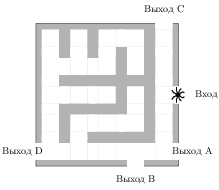
\includegraphics[scale=1.2]{323015.png}
}



\newpage
 \twocolumn[\section*{ ������� 5 ���2016.}]\setcounter{z}{0}

 �� ���� ������� ��������� ������ ���������.

\zad
  $-\dfrac37x=-5\dfrac47.$

\zad
   $\dfrac35x=12\dfrac35.$

\zad
   $\dfrac{1}{5x+10}=10.$

\zad
   $\dfrac{1}{x-6}=4.$


\zad
   $\dfrac{1}{2x+9}=\dfrac16.$

\zad
   $\dfrac{x-17}{x+1}=-5.$

\zad
   $\dfrac{x+58}{x-7}=-4.$

\zad
   $x=\dfrac{-9x+4}{x-6}.$
���� ��������� ����� ����� ������ �����, � ������ ������� ������� �� ���.

\zad
   $x=\dfrac{x+18}{x-6}.$
���� ��������� ����� ����� ������ �����, � ������ ������� ������� �� ���.

\zad   $\dfrac{x+8}{5x+7}=\dfrac{x+8}{7x+5}$. ���� ��������� ����� ����� ������ �����, � ������ �������� ������� �� ������.

\zad
  $2x^2-27x+88=0.$ ���� ��������� ����� ����� ������ �����, ������� ������� �� ���.

\zad
  $2x^2-27x+91=0.$ ���� ��������� ����� ����� ������ �����, ������� ������� �� ���.

\zad
  $x^2+9x+8=0.$ ���� ��������� ����� ����� ������ �����, ������� ������� �� ���.

\zad
  $x^2-8x=0.$ ���� ��������� ����� ����� ������ �����, ������� ������� �� ���.



\zad   $(x+6)^3=-729$.

\zad   $(x+1)^3=512$.


\zad   $(x-3)^5=-243$.


\zad   $(6-x)^7=-128$.

\zad
   $\sqrt{-3-6x}=3.$

\zad
   $\sqrt{69+5x}=8.$

\zad
   $\sqrt{-23-3x}=2.$

\zad
   $\sqrt{-40+7x}=3.$


\zad
 $\sqrt{\dfrac{14}{3x-30}}=\dfrac1{12}$.

\zad
  $\sqrt{\dfrac{16}{2x-10}}=\dfrac1{10}$.

\zad  $\sqrt{\dfrac{1}{15-4x}}=0,2$.

\zad  $\sqrt{\dfrac{1}{5-2x}}=\dfrac13$.

\zad
  $\sqrt{12+4x}=x.$ ���� ��������� ����� ����� ������ �����, ������� ������� �� ���.

\zad
  $\sqrt{-4+5x}=x.$ ���� ��������� ����� ����� ������ �����, ������� ������� �� ���.

\zad   $\sqrt{6+5x}=x$. ���� ��������� ����� ����� ������ �����, � ������ �������� ������� �� ������.


\zad
  $\sqrt[3]{x+2}=7$.

\zad
  $\sqrt[3]{x-2}=7$.

\zad
  $\sqrt[3]{x+9}=3$.

\zad
  $\sqrt[3]{x-10}=6$.



\zad  $\cos\dfrac{\pi(x+4)}{4}=\dfrac{\sqrt{2}}2$. � ������ �������� ���������� ������������� ������.

\zad
  $\cos\dfrac{\pi(2x-4)}{4}=\dfrac{\sqrt{2}}2$. � ������ �������� ���������� ������������� ������.

\zad   $\tg \dfrac{\pi x}{4}=-1$. � ������ �������� ���������� ������������� ������.

\zad   $\tg \dfrac{\pi (4x-3)}{6}=-\dfrac{1}{\sqrt{3}}$. � ������ �������� ���������� ������������� ������.

\zad   $\sin \dfrac{\pi x}{3}=0,5$. � ������ �������� ���������� ������������� ������.


\zad
  $\sin\dfrac{\pi(8x-5)}{3}=-\dfrac{\sqrt{3}}2$. � ������ �������� ���������� ������������� ������.

\zad
   $8^{6-x}=512.$

\zad
   $5^{-5-x}=25.$

\zad
  $\left( \dfrac{1}{3}\right)^{-x+4}= 3.$

\zad
  $\left( \dfrac{1}{49}\right)^{x-5}= 7.$

\zad
  $\left( \dfrac{1}{9}\right)^{4-x}= 729.$

\zad $ 8^{1+3x}= 64^{x}.$

\zad $ 5^{2+3x}= 25^{2x}.$

\zad $ 4^{13-4x}= 64^{3x}.$

\zad
  $2^{3+x}=0,4\cdot5^{3+x}$.


\zad
  $9^{3-x}=0,81\cdot 10^{3-x}$.


\zad
  $5^{4-3x}=2,5\cdot 2^{4-3x}$.


%\zad
%  $\log_4(-4+x)=1.$

\zad
  $\log_6(5-x)=3.$



\zad   $\log_5(x^2+2x)=\log_5(x^2+10).$

%\zad   $\log_7(x^2+2x)=\log_7(x^2+11).$


\zad   $\log_5(7-x)=\log_5(3-x)+1.$


\zad   $\log_4(2+7x)=\log_4(2+x)+1.$


%\zad   $\log_2(3-4x)=\log_2(1-4x)+1.$


\zad   $\log_{x-5}49=2$. ���� ���������
����� ����� ������ �����, � ������ ������� ������� �� ���.


%\zad   $\log_{x+3}64=3$. ���� ���������
%����� ����� ������ �����, � ������ ������� ������� �� ���.



%\zad   $\log_{x-5}32=5$. ���� ���������
%����� ����� ������ �����, � ������ ������� ������� �� ���.



\newpage
 \onecolumn \section*{ ������� 6 ���2016.}\setcounter{z}{0}


\zad 
� ������������ $ABC$ ���� $C$ ����� $90^{\circ}$, $\sin A=0,03$.
������� $\cos B$.


\zad 
� ������������ $ABC$ ���� $C$ ����� $90^{\circ}$, $\sin A=0,77$. ������� ������� �������� ���� ��� ������� $B$.


\zad 
� ������������ $ABC$ ���� $C$ ����� $90^{\circ}$, $AB=10$, $BC=6$. ������� $\sin A$.


\zad 
� ������������ $ABC$ ���� $C$ ����� $90^{\circ}$, $AC=4$, $\cos A=0,4$. ������� $AB$.

\zad 
� ������������ $ABC$ ���� $C$ ����� $90^{\circ}$, $AC=10$, $\tg A=0,7$. ������� $BC$.


\zad 
� ������������ $ABC$ ���� $C$ ����� $90^{\circ}$, $\tg A=\dfrac{2\sqrt{21}}{21}$. ������� $\cos B$.

\zad 
� ������������ $ABC$ ���� $C$ ����� $90^{\circ}$, $BC=25$, $\cos A=\dfrac{12}{13}$. ������� $AC$.

\zad 
� ������������ $ABC$ ���� $C$ ����� $90^{\circ}$, $AB=20$, $\tg A=\dfrac{4}{3}$.
 ������� $AC$.

\zad 
� ������������ $ABC$ ���� $C$ ����� $90^{\circ}$, $BC=12$, $\cos A=\dfrac{5\sqrt{41}}{41}$. ������� $AC$.


\zad 
� ������������ $ABC$ ���� $C$ ����� $90^{\circ}$, $\tg A=\dfrac{5}{12}$, $BC=2$.
������� $AB$.

\zad 
� ������������ $ABC$ ���� $C$ ����� $90^{\circ}$, $\sin A=\dfrac{2}{\sqrt{5}}$. ������� ������� �������� ���� ��� ������� $B$.

\zad 
� ������������ $ABC$ ���� $C$ ����� $90^{\circ}$, ������� �������� ���� ��� ������� $A$ ����� $-\dfrac35$, $AC=1,5$. ������� $BC$.

\zad 
� ������������ $ABC$ ���� $C$ ����� $90^{\circ}$, ������� �������� ���� ��� ������� $A$ ����� $-\dfrac{2\sqrt{29}}{29}$, $BC=4$. ������� $AC$.


\zad 
� ������������ $ABC$ ���� $C$ ����� $90^{\circ}$, $\cos A=\dfrac{\sqrt{19}}{10}$, $BC=9$. ������� $AB$.

\zad 
� ������������ $ABC$ ���� $C$ ����� $90^{\circ}$, $AB=2\sqrt{41}$, $BC=10$.
������� ������� �������� ���� ��� ������� $A$.

\zad 
� ������������ $ABC$ ���� $C$ ����� $90^{\circ}$, $\tg A=\dfrac{3\sqrt{7}}{7}$, $BC=9$.
 ������� $AB$.

\zad 
� ������������ $ABC$ $AC=BC=10$, $\sin B=\dfrac35$. ������� $AB$.


\zad 
� �������������� ������������ $ABC$ � ���������� $AC$
������� ������� $AB$ ����� 15, � $\cos A=\dfrac{4\sqrt{14}}{15}$. ������� ������, ����������� � ���������.



\zad 
� ������������ $ABC$ $AC=BC$, $AB=14$, $\cos A=0,7$. ������� $AC$.

\zad 
� ������������ $ABC$ $AC=BC$, ������ $CH$ ����� 7, $\cos A=0,96$. ������� $AC$.

\zad 
� ������������ $ABC$ $AC=BC$, ������ $CH$ ����� 12, $\tg A=\dfrac{\sqrt{20}}{5}$.
������� $AC$.


\zad 
� ������������ $ABC$ $AC=BC$, $AB=2$, ������ $AH$ ����� $\sqrt{3}$. ������� $\cos A$.


\zad 
� ������������ $ABC$ $AC=BC$, ������ $AH$ ����� 3, $BH=3\sqrt{15}$. ������� $\sin BAC$.

\zad 
� �������������� ������������ $ABC$ � ���������� $AC$
������� ������� $AB$ ����� 8, � $\cos A=\dfrac{\sqrt{7}}{4}$. ������� ������, ����������� � ���������.



\zad 
� ������������ $ABC$ ���� $C$ ����� $90^{\circ}$, $CH$  --- ������, $AC=5$, $AH=2\sqrt{6}$. ������� $\cos B$.

\zad 
� ������������ $ABC$ ���� $C$ ����� $90^{\circ}$, $AB=10\sqrt{3}$, $\sin A=0,5$. ������� ������ $CH$.

\zad 
� ������������ $ABC$ ���� $C$ ����� $90^{\circ}$, $CH$ --- ������, $AB=34$, $\tg A=\dfrac53$. ������� $BH$.

\zad 
� ������������ $ABC$ ���� $C$ ����� $90^{\circ}$, $CH$ --- ������, $BC=8$, $\cos A=\dfrac{\sqrt{15}}{4}$. ������� $BH$.

\zad 
� ������������ $ABC$ ���� $C$ ����� $90^{\circ}$, $CH$ --- ������, $BC=35$, $\sin A=\dfrac27$. ������� $AH$.





\zad (� 47207)
� ������������ $ABC$ $CD$ --- �������,  ���� $C$ ����� $90^{\circ}$, ���� $B$ ����� $39^{\circ}$. ������� ���� $ACD$. ����� ����� � ��������.



\zad (� 49209)
���� ���� ��������������� ������ ������� �� $102^{\circ}$. ������� ������� ����. ����� ����� � ��������.



\zad (� 54789)
����� ����������, ������ ������� ����� $2\sqrt{3}$, ������ ���������� �������������. ������� ������ ����������, ��������� ����� ����� ��������������.


\zad � ��������������� $ABCD$ $AB=3$, $AD=21$, $\sin A=\dfrac67$. ������� ������� ������ ���������������.

\zad � ��������������� $ ABCD$  $\cos A=\dfrac{\sqrt{51}}{10}$. ������� $\sin B$.

\zad ��������� �������������� �������� ����� 51 � 65. ������� ������� ����� 25. ������� ����� ������� ���� ��������.

\zad ��������� �������������� �������� ����� 43 � 73. ������� ������� ���� �������� ����� $\dfrac57$. ������� ������� �������.

\zad ������� ��������� �������������� �������� ����� 23. ������ �������� ����� 39. ������� ������� ���� ����� $\dfrac{13}{8}$. ������� ������� ���������.

\zad ������� ������� (����� � �������) ���� $AOB$. � ������ ������� �������� ��������, ���������� �� $2\sqrt{5}$.
\begin{center}
 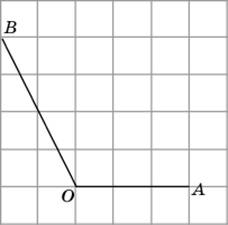
\includegraphics[scale=0.5]{27452.jpg}
 % 5085.png: 179x159 pixel, 72dpi, 6.32x5.61 cm, bb=0 0 179 159
\end{center}



\zad ������� ����� ���� $ AOB$. � ������ ������� �������� ������, ���������� �� $2\sqrt{2}$.
\begin{center}
 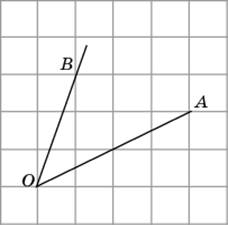
\includegraphics[scale=0.5]{27454.jpg}
 % 5085.png: 179x159 pixel, 72dpi, 6.32x5.61 cm, bb=0 0 179 159
\end{center}

\zad ���� �� ������� ����� ������������ ����� $85^{\circ}$. ����, �� ������� � ������ ������� �����, ��������� ��� $2:3$. ������� ���������� �� ���. ����� ����� � ��������.

\zad ���� ������������ ��������� ��� $2:3:4$. ������� ������� �� ���. ����� ����� � ��������.

\zad � ������������ $ABC$ $AC=BC$, $AD$ --- ������, ���� $BAD$ ����� $24^{\circ}$. ������� ���� $C$. ����� ����� � ��������.


\zad � ������������ $ABC$ $CD$ --- �������, ���� $ACB$ ����� $90^{\circ}$, ���� $B$ ����� $58^{\circ}$. ������� ���� $ACD$. ����� ����� � ��������.

\zad � ������������ $ABC$ ���� $C$ ����� $58^{\circ}$, $AD$ � $BE$  --- �����������, �������������� � ����� $O$. ������� ���� $AOB$. ����� ����� � ��������.

\zad � ������������� ������������ ���� ����� ������� � ������������, ������������ �� ������� ������� ����, ����� $21 ^{\circ}$. ������� ������� ���� ������� ������������. ����� ����� � ��������.

\zad � ������������ $ABC$ ���� $A$ ����� $60 ^{\circ}$, ���� $B$ ����� $82 ^{\circ}$. $AD$, $BE$ � $CF$  --- �����������, �������������� � ����� $O$. ������� ���� $AOF$. ����� ����� � ��������.

\zad � �������������� ������������ $ABC$ ������ $CH$ ����� $2\sqrt{3}$. ������� ������� ����� ������������.

\zad ������� ������ ������������ $ABC$, ��������� �� ������� $BC$, ���� ������� ���������� ������ ����� $\sqrt{5}$.
\begin{center}
\includegraphics[scale=0.5]{27804.jpg}
 % 5085.png: 179x159 pixel, 72dpi, 6.32x5.61 cm, bb=0 0 179 159
\end{center}

\zad ��������� �������� ����� 4 � 10. ������� ������� �� ��������, �� ������� ����� ������� ����� ���� �������� ���� �� �� ����������.

\zad ������� ������� ��������������� ������������ ����� 10. �� �����, ������ �� ��������� ����� ������������, ��������� ��� ������, ������������ ������� ��������. ������� �������� ������������� ���������������.

\zad ����������� ������ ���� ��������������� ����� ��������������� ������� � ��������� $4:3$, ������ �� ������� ������� ����. ������� ������� ������� ���������������, ���� ��� �������� ����� 88.

\zad �������������, ��������� �� ������� ������ ���� �� ������� ��������� �������������� ��������, ����� ��� �� �����, ������� ����� 10 � 4. ������� ������� ����� ���� ��������.

\zad ��������� �������� ����� 3 � 2. ������� �������, ����������� �������� ���������� ��������.

\zad ��������� ���������������� ����� 4 � 5. ������� �������� ����������������, ��������� �������� �������� �������� ������ ������� ����������������.

\zad ���� ����� ������ ��������� ����, ����������� �� �����, ������ ������� ����������? ����� ����� � ��������.

\zad ���� ����� ����� ��������� ����, ����������� �� �����, ������ ������� ����������? ����� ����� � ��������.

\zad ������ ���������� ����� 1. ������� �������� ������� (������)  ���������� ����, ������������ �� �����, ������ $\sqrt{2}$. ����� ����� � ��������.

\zad ����������� ���� �� $36 ^{\circ}$ ������ ������� ���������� ����, ������������ �� �� �� ���� ����������. ������� ��������� ����. ����� ����� � ��������.

\zad ������� ��������� ����, ����������� �� ����, ������� ���������� 20\% ����������. ����� ����� � ��������.

\zad ����� $AB$ ����� ���������� �� ��� �����, ��������� �������� ������� ��������� ��� $5:7$. ��� ����� ����� ����� ��� ����� �� ����� $C$, ������������� ������� ���� ����������? ����� ����� � ��������.

\zad ���� $A$ ���������������� $ABCD$, ���������� � ����������, ����� $58 ^{\circ}$. ������� ���� $C$ ����� ����������������. ����� ����� � ��������.

\zad ����� $A$, $B$, $C$, $D$, ������������� �� ����������, ����� ��� ���������� �� ������ ���� $AB$, $BC$, $CD$ � $AD$, ��������� �������� ������� ��������� �������������� ��� $4:2:3:6$. ������� ���� $A$ ���������������� $ABCD$. ����� ����� � ��������.

\zad ��������������� $ABCD$ ������ � ����������. ���� $ABC$ ����� $110 ^{\circ}
$, ���� $ABD$ ����� $70 ^{\circ}$. ������� ���� $CAD$. ����� ����� � ��������.

\zad ����� $AB$ ��������� ���� ���������� � $92 ^{\circ}$. ������� ���� $ABC$ ����� ���� ������ � ����������� � ����������, ����������� ����� ����� $B$. ����� ����� � ��������.

\zad ���� ����� ������ $AB$ � ����������� $BC$ � ���������� ����� $32 ^{\circ}$. ������� �������� ������� ����, ����������� ������ $AB$. ����� ����� � ��������.

\zad ����� ����� $A$, $B$ ���� ���������� � $62 ^{\circ}$ ��������� ����������� $AC$ � $BC$. ������� ���� $ACB$. ����� ����� � ��������.

\zad ���� $ACO$ ����� $28 ^{\circ}$, ��� $O$ --- ����� ����������. ��� ������� $CA$ �������� ����������. ������� �������� ������� ���� $AB$ ����������, ����������� ������ ����� ����. ����� ����� � ��������.

\zad ������� ���� $ACB$, ���� ��������� ���� $ADB$ � $DAE$ ��������� �� ���� ����������, ��������� �������� ������� ����� �������������� $118 ^{\circ}$ � $38 ^{\circ}$. ����� ����� � ��������.
\begin{center}
\includegraphics[scale=0.5]{27885.jpg}
 % 5085.png: 179x159 pixel, 72dpi, 6.32x5.61 cm, bb=0 0 179 159
\end{center}

\zad ������� �������� ���� $ABC$. ����� ����� � ��������.
\begin{center}
\includegraphics[scale=0.5]{27889.jpg}
 % 5085.png: 179x159 pixel, 72dpi, 6.32x5.61 cm, bb=0 0 179 159
\end{center}

\zad ������� ����������� ������������ ����� $\sqrt{3}$. ������� ������ ����������, ��������� ����� ����� ������������.

\zad ���������� �������������� ������������ ����� 12. ������� ������ ��������� ���������� ����� ������������.

\zad ������� ������� ��������������� ������������ ����� 1, ���� ��� �������, �������������� ���������, ����� $120 ^{\circ}$. ������� ������� ��������� ���������� ����� ������������.

\zad ���� ����� ������� ����������� ��������������, ���������� � ����������, ������ ������� ����� 6?

\zad ������� ������ ����������, ��������� � ���������� �����������, ������ �������� ����� 6.

\zad ������ ����������, ��������� � ���������� �����������, ����� $\dfrac{\sqrt{3}}{6}$. ������� ������� ����� ������������.

\zad ������� ����� ����� 1, ������ ���� ����� $30 ^{\circ}$. ������� ������ ��������� ���������� ����� �����.

\zad ������� ������ ��������, � ������� ������� ���������� ������� 1.

\zad ������� ������� ����������� ��������������, ���������� ����� ����������, ������ ������� ����� $\sqrt{3}$.

\zad ������� $AB$ ������������ $ABC$ ����� 1. �������������� �� ���� $C$ ����� $30 ^{\circ}$. ������� ������ ����������, ��������� ����� ����� ������������.

\zad ������� $AB$  ������������ $ABC$ ����� ������� ��������� ����� ���� ����������. ������� ���� $C$, ���� ��������, ��� �� �����. ����� ����� � ��������.

\zad ������� ������� ��������������� ������������ ����� 40, ��������� ����� 48. ������� ������ ��������� ���������� ����� ������������.

\zad ����� �������� ������� ����������. �������� �������� ����� 22, ������� ����� ����� 5. ������� ������� ������� ��������.

\zad ������� ������� �������������� �������� ����� �� �������� ���������, ���� ��� ��������� ����� $60 ^{\circ}$, ������� ��������� ����� 12. ������� ������ ��������� ���������� ���� ��������.

\zad ���� $A$, $B$ � $C$ ���������������� $ABCD$ ��������� ��� $1:2:3$. ������� ���� $D$, ���� ����� ������� ���������������� ����� ������� ����������. ����� ����� � ��������.

\zad �������� ����������� �������������� ����� 72. ������� ������� ��������� ����������.

\zad ���� ����� �������� ����������� $n$-���������, ���������� � ����������, � �������� ���� ����������, ����������� � ���� �� ������ �������, ����� $54 ^{\circ}$. ������� $n$.

\zad ������ ��������������� �������������� ������������ ����� $2+\sqrt{2}$. ������� ������ ����������, ��������� � ���� �����������.

\zad ����������, ��������� � �������������� �����������, ����� � ����� ������� ���� �� ������� ������ �� ��� �������, ����� ������� ����� 5 � 3, ������ �� �������, �������������� ���������. ������� �������� ������������.

\zad ������� ������� ��������, ��������� ����� ����������, ����� 3 � 5. ������� ������� ����� ��������.

\zad ����� ���������� ������� ��������, �������� ������� ����� 40. ������� �� ������� �����.

\zad  �������� ������������� ��������, ��������� ����� ����������, ����� 22, �� ������� ������� ������� ����� 7. ������� ������ ����������.

\zad �������� ����������������, ���������� ����� ����������, ����� 24, ��� ��� ������� ����� 5 � 6. ������� ������� �� ���������� ������.


\zad ��� ������� ���������� ����� ���������� ���������������� ��������� (� ���������������� �������) ��� $1:2:3$. ������� ������� ������� ����� ����������������, ���� ��������, ��� ��� �������� ����� 32.

\zad � ����������, ��������� � ����������� $ABC$, ��������� ��� �����������. ��������� ���������� ������������� ����� 6, 8, 10. ������� �������� ������� ������������.

\zad ����� ����������, ������ ������� ����� $\sqrt{8}$, ������ �������. ������� ������ ����������, ��������� ����� ����� ��������.


 

\parbox[b][25mm][t]{120mm}{ \zad ������� ������ ����������, ��������� � ����������� $ABC$, ������ ������� ���������� ������ ������� 1.
}
\hfill
\parbox[b][32mm][t]{40mm}{
  \includegraphics[scale=0.5]{27951.jpg}
}



% \zad ��������� �������������� �������� ����� 6 � 12. ����� ������� ���� �������� ����� 0,8. ������� ������� �������.
% 
% \zad ������� ����������� ���� $AOB$, ���� �� �� $15 ^{\circ}$ ������ ���������� ���� $ACB$, ������������ �� �� �� ����.
% 
% \zad � ����� $ABCD$ ���� $ACD$ ����� $43 ^{\circ}$. ������� ���� $ABC$. ����� ����� � ��������.

\newpage
 \twocolumn[\section*{ ������� 7 ���2016.}] \setcounter{z}{0}


\par \zad (� 6877)
�� ������� ��������� ������ ������� $y=f(x)$, ������������ �� ��������� $(-2; 11)$. ���������� ���������� ����� �����, � ������� ����������� ������� ������������.
\begin{center}
 \includegraphics[scale=0.7]{6877.png}
 % 6877.png: 241x155 pixel, 72dpi, 8.50x5.47 cm, bb=0 0 241 155
\end{center}


\par \zad (� 6881)
�� ������� ��������� ������ ������� $y=f(x)$, ������������ �� ��������� $(-6; 5)$. ���������� ���������� ����� �����, � ������� ����������� ������� ������������.
\begin{center}
 \includegraphics[scale=0.7]{6881.png}
 \end{center}

\par \zad (� 6997)
�� ������� ��������� ������ ������� $y=f(x)$, ������������ �� ��������� $(-7; 5)$. ���������� ���������� ����� �����, � ������� ����������� ������� ������������.
\begin{center}
 \includegraphics[scale=0.7]{6997.png}
 \end{center}
\par \zad (� 7117)
�� ������� ��������� ������ ������� $y=f(x)$, ������������ �� ��������� $(-6; 6)$. ������� ���������� �����, � ������� ����������� � ������� ������� ����������� ������ $y=-12.$
\begin{center}
 \includegraphics[scale=0.7]{7117.png}
 \end{center}
\par \zad (� 7119)
�� ������� ��������� ������ ������� $y=f(x)$, ������������ �� ��������� $(-10; 4)$. ������� ���������� �����, � ������� ����������� � ������� ������� ����������� ������ $y=8$.
\begin{center}
 \includegraphics[scale=0.7]{7119.png}
 \end{center}
\par \zad (� 7357)
�� ������� ��������� ������ ������� $y=f(x)$, ������������ �� ��������� $(-9; 4)$. ������� ����� ����� ���������� ������� $f(x)$.
\begin{center}
 \includegraphics[scale=0.7]{7357.png}
 \end{center}
\par \zad (� 7557)
�� ������� ��������� ������ ����������� ������� $f(x)$, ������������ �� ��������� $(-8; 4)$. � ����� ����� ������� $[-5; -3 ]$ $f(x)$ ��������� ���������� ��������?
\begin{center}
 \includegraphics[scale=0.7]{7557.png}
 \end{center}
\par \zad (� 7563)
�� ������� ��������� ������ ����������� ������� $f(x)$, ������������ �� ��������� $(-8; 3)$. � ����� ����� ������� $[0; 2 ]$ $f(x)$ ��������� ���������� ��������?
\begin{center}
 \includegraphics[scale=0.7]{7563.png}
 \end{center}

 \zad (� 6427)
�� ������� ��������� ������ ����������� ������� $f(x)$, ������������ �� ��������� $(-5;5)$. ������� ���������� ����� ���������� ������� $f(x)$ �� ������� $[-4;4]$.
\begin{center}
 \includegraphics[scale=0.5]{6427.jpg}
 % 6427.jpg: 486x348 pixel, 96dpi, 12.86x9.21 cm, bb=0 0 365 261
\end{center}
\par \zad (� 7957)
�� ������� ��������� ������ ����������� ������� $f(x)$, ������������ �� ��������� $(-8; 13)$. ������� ���������� ����� ���������� ������� $f(x)$ �� ������� $[-5;12]$.
\begin{center}
 \includegraphics[scale=0.6]{7957.png}
 \end{center}
\par \zad (� 7961)
�� ������� ��������� ������ ����������� ������� $f(x)$, ������������ �� ��������� $(-10; 12)$. ������� ���������� ����� ���������� ������� $f(x)$ �� ������� $[-9;10]$.
\begin{center}
 \includegraphics[scale=0.6]{7961.png}
 \end{center}
\par \zad (� 8157)
�� ������� ��������� ������ ����������� ������� $f(x)$, ������������ �� ��������� $(-1; 12)$. ������� ���������� �������� ������� $f(x)$. � ������ ������� ����� ����� �����, �������� � ��� ����������.
\begin{center}
 \includegraphics[scale=0.7]{8157.png}
 \end{center}
\par \zad (� 8163)
�� ������� ��������� ������ ����������� ������� $f(x)$, ������������ �� ��������� $(-5; 7)$. ������� ���������� ����������� ������� $f(x)$. � ������ ������� ����� ����� �����, �������� � ��� ����������.
\begin{center}
 \includegraphics[scale=0.7]{8163.png}
 \end{center}
\par \zad (� 8357)
�� ������� ��������� ������ ����������� ������� $f(x)$, ������������ �� ��������� $(-1; 15)$. ������� ���������� ����������� ������� $f(x)$. � ������ ������� ����� ����������� �� ���.
\begin{center}
 \includegraphics[scale=0.7]{8357.png}
 \end{center}
\par \zad (� 8557)
�� ������� ��������� ������ ����������� ������� $f(x)$, ������������ �� ��������� $(-7; 7)$. ������� ���������� �����, � ������� ����������� � ������� ������� $f(x)$ ����������� ������ $y=-2x -19$ ��� ��������� � ���.
\begin{center}
 \includegraphics[scale=0.7]{8557.png}
 \end{center}
\par \zad (� 8563)
�� ������� ��������� ������ ����������� ������� $f(x)$, ������������ �� ��������� (-6; 8). ������� ���������� �����, � ������� ����������� � ������� ������� $f(x)$ ����������� ������ $y=-x -3$ ��� ��������� � ���.
\begin{center}
 \includegraphics[scale=0.7]{8563.png}
 \end{center}
\par \zad (� 8957)
�� ������� ��������� ������ ����������� ������� $f(x)$, ������������ �� ��������� $(-1; 11)$. ������� ����� ���������� ������� $f(x)$ �� ������� $[5; 10 ]$.
\begin{center}
 \includegraphics[scale=0.7]{8957.png}
 \end{center}
\par \zad (� 8965)
�� ������� ��������� ������ ����������� ������� $f(x)$, ������������ �� ��������� $(-3; 8).$ ������� ����� ���������� ������� $f(x)$ �� ������� $[0; 7 ].$
\begin{center}
 \includegraphics[scale=0.7]{8965.png}
 \end{center}
\par \zad (� 9157)
�� ������� �������� ������ ������� $y=f(x)$ � ����������� � ���� � ����� � ��������� $x_0$. ������� �������� ����������� ������� $f(x)$ � ����� $x_0$.
\begin{center}
 \includegraphics[scale=0.7]{9157.png}
 \end{center}
\par \zad (� 9161)
�� ������� �������� ������ ������� $y=f(x)$ � ����������� � ���� � ����� � ��������� $x_0$. ������� �������� ����������� ������� $f(x)$ � ����� $x_0$.
\begin{center}
 \includegraphics[scale=0.7]{9161.png}
 \end{center}
\par \zad (� 9359)
�� ������� �������� ������ ������� $y=f(x)$ � ����������� � ���� � ����� � ��������� $x_0$. ������� �������� ����������� ������� $f(x)$ � ����� $x_0$.
\begin{center}
 \includegraphics[scale=0.7]{9359.png}
 \end{center}

\par \zad (� 54801)
�� ������� ��������� ������ ������� $y~=~f(x)$. ������, ���������� ����� ������ ���������, �������� ������� ���� ������� � ����� � ��������� 10. ������� $f'(10).$
\begin{center}
 \includegraphics[scale=0.5]{54801.png}
 % 54801.png: 442x356 pixel, 72dpi, 15.59x12.56 cm, bb=0 0 442 356
\end{center}

\par \zad

������ $y~=~7x-5$ ����������� ����������� � ������� ������� $y~=~x^2+6x-8$. ������� �������� ����� �������.

\zad
������ $y=3x+1$ �������� ����������� � ������� ������� $ax^2+2x+3$. ������� $a$.

\zad ������ $y=-5x+8$ �������� ����������� � ������� ������� $28x^2+bx+15$. ������� $b$, ��������, ��� �������� ����� ������� ������ 0.



\zad ������������ ����� �������� ������������ �� ������ $x(t)=\dfrac12t^3-3t^2+2t$, ��� $x$ --- ���������� �� ����� ������� � ������, $t$ --- ����� � ��������, ���������� � ������ ��������. ������� �� �������� (� ������ � �������) � ������ ������� $t=6$�.


\zad ������������ ����� �������� ������������ �� ������ $x(t)=t^2-13t+23$, ��� $x$ --- ���������� �� ����� ������� � ������, $t$ --- ����� � ��������, ���������� � ������ ��������. � ����� ������ ������� (� ��������) �� �������� ���� ����� 3 �/�?



\zad (� 122719)
������������ ����� �������� ������������ �� ������ $x(t)=-\dfrac12t^4+3t^3+t^2-9$, ��� $x$ --- ���������� �� ����� ������� � ������, $t$ --- ����� � ��������, ���������� � ������ ��������. ������� �� �������� (� ������ � �������) � ������ ������� $t=4$~�.

\zad (� 123719)
������������ ����� �������� ������������ �� ������$x(t)=\dfrac13t^3+6t^2+8t-17$, ��� $x$ --- ���������� �� ����� ������� � ������, $t$ --- ����� � ��������, ���������� � ������ ��������. � ����� ������ ������� (� ��������) �� �������� ���� ����� 93 �/�?

\zad (� 317547)
�� ������� �������� ������ ������� $y=f(x)$ � ������ ����� �� ��� �������: $x_1$, $x_2$, $x_3$, \ldots, $x_{10}$. � �������� �� ���� ����� ����������� ������� $f(x)$ ������������?
\begin{center}
 \includegraphics[scale=0.7]{317547.png}
 % 6877.png: 241x155 pixel, 72dpi, 8.50x5.47 cm, bb=0 0 241 155
\end{center}

%\zad (� 317559)
%�� ������� �������� ������ �������  $y=f(x)$ � ������ ����� �� ��� �������: $x_1$, $x_2$, $x_3$, \ldots, $x_8$. � �������� �� ���� ����� ����������� �������  $f(x)$ ������������?
%\begin{center}
% \includegraphics[scale=0.7]{317559.png}
% % 6877.png: 241x155 pixel, 72dpi, 8.50x5.47 cm, bb=0 0 241 155
%\end{center}


\zad (� 317745)
�� ������� �������� ������ $y=f'(x)$ ����������� ������� $f(x)$ � ����� ����� �� ��� �������:  $x_1$, $x_2$, $x_3$, \ldots, $x_6$. � �������� �� ���� ����� ������� $f(x)$ ����������?
\begin{center}
 \includegraphics[scale=0.7]{317745.png}
 % 6877.png: 241x155 pixel, 72dpi, 8.50x5.47 cm, bb=0 0 241 155
\end{center}


%\zad (� 317749)
%�� ������� �������� ������ $y=f'(x)$ ����������� ������� $f(x)$   � ������ ����� �� ��� �������:  $x_1$, $x_2$, $x_3$, \ldots, $x_9$. � �������� �� ���� ����� ������� $f(x)$  ����������?
%\begin{center}
% \includegraphics[scale=0.7]{317749.png}
% % 6877.png: 241x155 pixel, 72dpi, 8.50x5.47 cm, bb=0 0 241 155
%\end{center}


\zad (� 317849)
�� ������� �������� ������ $y=f'(x)$ ����������� ������� $f(x)$ � ����� ����� �� ��� �������:  $x_1$, $x_2$, $x_3$, \ldots, $x_6$. � �������� �� ���� ����� �������  �������?
\begin{center}
 \includegraphics[scale=0.7]{317849.png}
 % 6877.png: 241x155 pixel, 72dpi, 8.50x5.47 cm, bb=0 0 241 155
\end{center}


%\zad (� 317947)
%�� ������� ��������� ������ �������  $f(x)$  � �������� ����� $-2$, $-1$, 2, 4. � ����� �� ���� ����� �������� ����������� ����������? � ������ ������� ��� �����.
%\begin{center}
% \includegraphics[scale=0.7]{317947.png}
% % 6877.png: 241x155 pixel, 72dpi, 8.50x5.47 cm, bb=0 0 241 155
%\end{center}


\zad (� 317949)
�� ������� ��������� ������ �������  $f(x)$  � �������� ����� $-2$, 1, 3, 4. � ����� �� ���� ����� �������� ����������� ����������? � ������ ������� ��� �����.
\begin{center}
 \includegraphics[scale=0.7]{317949.png}
 % 6877.png: 241x155 pixel, 72dpi, 8.50x5.47 cm, bb=0 0 241 155
\end{center}


\zad (� 318045)
�� ������� ��������� ������ �������  $f(x)$  � �������� ����� $-1$, 1, 2, 4. � ����� �� ���� ����� �������� ����������� ����������? � ������ ������� ��� �����.
\begin{center}
 \includegraphics[scale=0.7]{318045.png}
 % 6877.png: 241x155 pixel, 72dpi, 8.50x5.47 cm, bb=0 0 241 155
\end{center}

%
%\zad (� 318049)
%�� ������� ��������� ������ �������  $f(x)$  � �������� ����� $-2$, $-1$, 1, 3. � ����� �� ���� ����� �������� ����������� ����������? � ������ ������� ��� �����.
%\begin{center}
% \includegraphics[scale=0.7]{318049.png}
% % 6877.png: 241x155 pixel, 72dpi, 8.50x5.47 cm, bb=0 0 241 155
%\end{center}


\zad (� 323081)
�� ������� �������� ������ ������� $y=F(x)$  ����� �� ������������� ��������� ������� $f(x)$, ����������� �� ��������� $(-2;6)$. ��������� ��������, ���������� ���������� ������� ��������� $f(x)=0$ �� ������� $[-1;5]$.
\begin{center}
 \includegraphics[scale=0.7]{323081.png}
 % 6877.png: 241x155 pixel, 72dpi, 8.50x5.47 cm, bb=0 0 241 155
\end{center}



\zad (� 323179)
�� ������� �������� ������ ������� $y=F(x)$  ����� �� ������������� ��������� ������� $f(x)$, ����������� �� ��������� $(-2;4)$. ��������� ��������, ���������� ���������� ������� ��������� $f(x)=0$ �� ������� $[-1;3]$.
\begin{center}
 \includegraphics[scale=0.7]{323179.png}
 % 6877.png: 241x155 pixel, 72dpi, 8.50x5.47 cm, bb=0 0 241 155
\end{center}



\zad (� 323183)
�� ������� �������� ������ ��������� ������� $y=f(x)$ (��� ���� � ����� ��������� ������). ��������� ��������, ��������� $F(6)-F(2)$, ��� $F(x)$ --- ���� �� ������������� ������� $f(x)$.
\begin{center}
 \includegraphics[scale=0.7]{323183.png}
 % 6877.png: 241x155 pixel, 72dpi, 8.50x5.47 cm, bb=0 0 241 155
\end{center}



\zad (� 323187)
�� ������� �������� ������ ��������� ������� $y=f(x)$ (��� ���� � ����� ��������� ������). ��������� ��������, ��������� $F(6)-F(4)$, ��� $F(x)$ --- ���� �� ������������� ������� $f(x)$.
\begin{center}
 \includegraphics[scale=0.7]{323187.png}
 % 6877.png: 241x155 pixel, 72dpi, 8.50x5.47 cm, bb=0 0 241 155
\end{center}



%\zad (� 323293)
%�� ������� �������� ������ ��������� �������  $y=f(x)$. ������� $F(x)=x^3+24x^2+195x-\dfrac34$ --- ���� �� ������������� ������� $f(x)$. ������� ������� ����������� ������.
%\begin{center}
% \includegraphics[scale=0.7]{323293.png}
% % 6877.png: 241x155 pixel, 72dpi, 8.50x5.47 cm, bb=0 0 241 155
%\end{center}


\zad (� 323383)
�� ������� �������� ������ ��������� �������  $y=f(x)$. ������� $F(x)=-\dfrac49x^3-\dfrac{34}{3}x^2-\dfrac{280}{3}x-\dfrac{18}{5}$ --- ���� �� ������������� ������� $f(x)$. ������� ������� ����������� ������.
\begin{center}
 \includegraphics[scale=0.7]{323383.png}
 % 6877.png: 241x155 pixel, 72dpi, 8.50x5.47 cm, bb=0 0 241 155
\end{center}


\zad (� 323385)
�� ������� �������� ������ ��������� �������  $y=f(x)$. ������� $F(x)=-\dfrac16x^3-\dfrac{17}{4}x^2-35x-\dfrac{5}{11}$ --- ���� �� ������������� ������� $f(x)$. ������� ������� ����������� ������.
\begin{center}
 \includegraphics[scale=0.7]{323385.png}
 % 6877.png: 241x155 pixel, 72dpi, 8.50x5.47 cm, bb=0 0 241 155
\end{center}

















\newpage
 \onecolumn\section*{������� 8 ���2016.}
\setcounter{z}{0}

\zad
������������� �������������� ������ ����� ��������, ������ ��������� � ������ �������� ����� 6. ������� ����� ���������������.


\zad
������������� �������������� ������ ����� ��������, ������ ��������� �������� ����� 3. ����� ��������������� ����� 27. ������� ������ ��������.

\zad
������������� �������������� ������ ����� ����� ������� 9,5. ������� ��� �����.

\zad
� �����, ������� ����� ���������� ����������� ������, ������ ����. ������� ���� ��������� 80 ��. �� ����� ������ ����� ���������� ������� ����, ���� �� �������� � ������ ����� �� �����, � �������� ������� ��������� � 4 ���� ������, ��� � �������?


\zad
� ��������� ������ ������ ����� ������������� ����������� � �������� 9 � 6. ������� ����� ����� $\dfrac{2}{\pi }$. ������� ����� ��������, ���������� ����� ���� ������.


\zad
������� � ����� ����� ����� ��������� � ����� ������. ��������� ����� ��������, ���� ����� ������ ����� 25.


\zad
����� ������ ����� 128. ����� �������� ������ ����������� ��������� ������ ��������� �������, ������� �������� ���������� �������� ������ � ��� �� ��������. ������� ����� �������� ������.


\zad
��� ����� �������������� ���������������, ��������� �� ����� �������, ����� 3 � 4. ������� ����������� ����� ��������������� ����� 94. ������� ������ �����, ��������� �� ��� �� �������.


\zad
������� ����������� ���� ����� 18. ������� ��� ���������.

\zad
����� ���� ����� 8. ������� ������� ��� �����������.


\zad
������� ������� ������� ����������� ���������� ������������� ������, ������� ��������� ������� ����� 5, � ������ --- 10.


\zad
 ������ ��������� �������� ����� 2, ������ ����� 3. ������� ������� ������� ����������� ��������, �������� �� $\pi$.


\zad
 ������� �������� ����� ���� ����� 3. ������� ������� ����������� ����.

\zad
��� ����� �������������� ���������������, ��������� �� ����� �������, ����� 1, 2. ������� ����������� ��������������� ����� 16. ������� ��� ���������.


\zad
���� ������ ����� ���� ��������� �� 1, �� ��� ������� ����������� ���������� �� 54. ������� ����� ����.

\zad
������� ������� ����������� ������ ������, � ��������� ������� ����� ���� � �����������, ������� 6 � 8, � ������� ������, ������ 10.

\zad
������� ������� ����� ���������� ��������������� ������, ���� ������� �� ��������� ����� 20, � ������� ����������� ����� 1760.


\zad ������� ������� ������� ����������� ���������� ����������� ������, ��������� ����� ��������, ������ ��������� �������� �����
$\sqrt{3}$, � ������ ����� 2.


\zad
������� ������� ������� ����������� ���������� ������������� ������, ��������� ����� ��������, ������ ��������� �������� ����� $\sqrt{3}$, � ������ ����� 2.


\zad
������������� �������������� ������ ����� ��������� �����. ������� ��� ������� �����������.

\zad
����� ������� ����� ��������� ����������� ������, ������� ������� ����������� ������� ����� 24, ��������� ���������, ������������ �������� �����. ������� ������� ������� ����������� ���������� ����������� ������.

\zad
������� ��������� ���������� ��������������� �������� ����� 10, ������� ����� ����� 13. ������� ������� ����������� ���� ��������.

\zad
�� ������� ��� ���������� ������� ����������� ����, ���� ������ ���� ��������� � 2 ����?

\zad
����� ���� ������ �������, ������� ����������� �������� ����� 18. ������� ������� ����������� ����.

\zad
����� ��������������� $ABCDA_1B_1C_1D_1$  ����� 9. ������� ����� ����������� �������� $ABCA_1.$

 \zad
 �� ���������� ���� �������� ���������� ��������������� ������ �� �������� ��������� 0,5 � ������� ������ 1. ������� ������� ����������� ���������� ����� ����.


\par \zad
����� �������������� ��������������� ����� 72. ���� �� ��� ����� ����� 3. ������� ������� ����� ���������������, ���������������� ����� �����.
\par \zad
������� ������ ���������� ����������� ��������, ������� ��������� ������� ����� 5, � ����� ����� $6\sqrt{3}$.
\par \zad
��� ����� �������������� ���������������, ��������� �� ����� �������, ����� 32 � 42. ��������� ��������������� ����� 58. ������� ����� ���������������.
\par \zad
������� ����� ������, � ���������� ������� ����� ���������� �������������� �� ��������� 4, � ������� ����� ����� $6\sqrt{3}$ � ��������� � ��������� ��������� ��� ����� $30^\circ$.
\par \zad
����� ���������� ��������������� �������� $SABCD$ ����� 136. ����� $E$ --- �������� ����� $SB$. ������� ����� ����������� �������� $EABC$.
\par \zad
������ ������ ����� 2, ���������� ����� 4. ������� ��� �����, �������� �� $\pi $.
\par \zad
����� ���������� ��� �������� ��������������� �������������� ������������ $ABC$ ������ ������, ������� 6. ������� ��� �����, �������� �� $\pi $.
\par \zad
���������� ������ ����������� ������ ������ ������������� ����������� � �������� 15 � 20, ������ ������ ����� 17. ������� ������� �� �����������.
\par \zad
� ����������� ������ ��� ������� ����� ���������������. �� ����� ����� ����� 8 � ������� �� ������ ������� ����� �� 10 � 24. ������� ������� ������� ����������� ���� ������.
\par \zad
������� ������� ������� ����������� ���������� ����������� ������, ��������� � �������, ������ ��������� �������� ����� $2\sqrt{3}$, � ������ ����� 4.
\par \zad
����� ��������� ����� 4,7. ������� ����� �������������, ��������� �������� �������� �������� ������ ������� ���������.


\zad
����� ���������� ��������� �������� ����� 6, ������ ����� 4. ������� ������� ������� ����������� ��������.


\zad
����� ���������� ��������� ������ ����� 6, ���������� ����� 2. ������� ������� ������� ����������� ������.

\zad
�� ������� ��� ���������� ������� ������� ����������� ������, ���� ��� ���������� ��������� � 1,5 ����?

\zad
� ��������� ������ ������ ����� ���� � �����������, ������� 9 � 12. ������� �� ����������� ����� 318. ������� ������� ����� ���� ������.

\zad
����� ������� ����� ��������� ����������� ������ ��������� ���������, ������������ �������� �����. ������� ������� ����������� ���������� ����������� ������ ����� 18. ������� ������� ������� ����������� �������� ������.

\zad
������� ������� ������� �������� ����� 5. ������� ������� ������� ����������� ��������, �������� �� $\pi$.

\zad
����� ���������� ������������� �������� 40,5. ������� ��������� ����� 3. ������� ������� �����.

\zad
�������� ����� ���� �� �������� 3,7 �������� ������� ���� ������� 1,85. ������� ������� $S$ ����� ����������� ����, ������� ������ ����. � ������ �������� $\dfrac{S}{\pi}$.

\zad
������� ����� �������������, ��������� �������� �������� �����  $A$, $B$, $B_1$, $D_1$  ��������������� $ABCDA_1B_1C_1D_1$, � �������� $AB=3$, $AD=8$, $AA_1=8$.


\zad
������� ����� �������������, ��������� �������� �������� �����  $C$, $A_1$, $B_1$, $C_1$, $D_1$, $E_1$, $F_1$ ���������� ������������� ������ $ABCDEFA_1B_1C_1D_1E_1F_1$, ������� ��������� ������� ����� 9, � ������� ����� ����� 5.

\zad
������� ����� �������������, ��������� �������� �������� ����� $A$, $C$, $D$, $F$, $A_1$,  $C_1$, $D_1$, $F_1$  ���������� ������������� ������ $ABCDEFA_1B_1C_1D_1E_1F_1$, ������� ��������� ������� ����� 8, � ������� ����� ����� 9.


\zad
����� ���������� ��������� �������� ����� 7. ������� ������� ����������� ����� 105. ������� ������ ��������.









\zad
������������� �������������� ������ ����� ��������, ������ ��������� � ������ �������� ����� 9,5. ������� ����� ���������������.

\zad ������������� �������������� ������ ����� ��������, ������ ��������� �������� ����� 4. ����� ��������������� ����� 16. ������� ������ ��������.

\zad
� �����, ������� ����� ���������� ����������� ������, ������ ����. ������� ���� ��������� 18 ��. �� ����� ������ ����� ���������� ������� ����, ���� �� �������� � ������ ����� �� �����, � �������� ������� ��������� � 3 ���� ������, ��� � �������?

\zad � ��������� ������ ������ ����� ������������� ����������� � �������� 6 � 8. ������� ����� ����� $\dfrac{5}{\pi }$. ������� ����� ��������, ���������� ����� ���� ������.

\zad
������� � ����� ����� ����� ��������� � ����� ������. ��������� ����� ��������, ���� ����� ������ ����� 18.

\zad ����� ������ ����� 16. ����� �������� ������ ����������� ��������� ������ ��������� �������, ������� �������� ���������� �������� ������ � ��� �� ��������. ������� ����� �������� ������.

\zad
������� ��������� ���������� ������������� �������� ����� 10, ������� ����� ����� 13. ������� ������� ������� ����������� ���� ��������.

\zad
������� ������� ������� ����������� ���������� ����������� ������, ��������� ����� ��������, ������ ��������� �������� ����� $\sqrt{0,12}$, � ������ ����� 4.





\zad
����� ���������� ��������� �������� ����� 6, ������ ����� 4. ������� ������� ������� ����������� ��������.

\zad
�� ������� ��� ���������� ������� ������� ����������� ������, ���� ������ ��� ��������� ��������� � 4 ����?

\zad
��� ����� �������������� ���������������, ��������� �� ����� �������, ����� 12 � 8. ����� ��������������� ����� 960. ������� ������� ��� �����������.


\zad
������� ������� ����������� ���������� ��������������� ��������,  ������� ��������� ������� ����� 48 � ������ ����� 7.

\zad
������ ��������� ������ ����� 24, ������ ����� 7. ������� ������� ������ ����������� ������, �������� �� $\pi$.


\zad
������� ����� �������������, ��������� �������� �������� �����  $A$, $B$, $A_1$, $B_1$, $C_1$  ��������������� $ABCDA_1B_1C_1D_1$, � �������� $AB=9$, $AD=5$, $AA_1=9$.

\zad
������� ����� �������������, ��������� �������� �������� �����  $A$, $B$, $D$, $D_1$  ��������������� $ABCDA_1B_1C_1D_1$, � �������� $AB=7$, $AD=8$, $AA_1=9$.


\zad
������� ����� �������������, ��������� �������� �������� ����� $B$, $C$, $A_1$, $B_1$, $C_1$ ���������� ����������� ������ $ABCA_1B_1C_1$,  ������� ��������� ������� ����� 6, � ������� ����� ����� 5.

\zad
������� ����� �������������, ��������� �������� �������� ����� $A$, $C$, $B_1$, $C_1$ ���������� ����������� ������ $ABCA_1B_1C_1$,  ������� ��������� ������� ����� 6, � ������� ����� ����� 8.

\zad
������� ����� �������������, ��������� �������� �������� ����� $A$, $B$, $C$, $D$, $A_1$, $B_1$, $C_1$, $D_1$  ���������� ������������� ������ $ABCDEFA_1B_1C_1D_1E_1F_1$, ������� ��������� ������� ����� 14, � ������� ����� ����� 6.

\zad
������� ����� �������������, ��������� �������� �������� ����� $A_1$, $E_1$, $F_1$, $F$ ���������� ������������� ������ $ABCDEFA_1B_1C_1D_1E_1F_1$, ������� ��������� ������� ����� 9, � ������� ����� ����� 12.

\zad
���������� ��������������� ������ ������� ����� ��������, ������ ��������� �������� ����� 6. ������� ������� ����������� ������ ����� 96. ������� ������ ��������.

\zad (� 269905)

������� ����� ��������, ������������ �� �������. �� ���������� �������� �������������, �������� ������� �������� ���������������, � ���� �� ������� ����� ��������������� ��������� ��������� � ����� 6.

\begin{center}
 \includegraphics[scale=1.1]{269905.png}
 \end{center}

\newpage

\zad (� 270573)
������� ������� ���������� ����� ��������� $B$ � $D_1$ �������������� ���������������, ��� �������� $AB=4$, $AD=6$, $AA_1=5$.

\zad  (� 271179)
������� ���������� ����� ��������� $A$ � $D_1$ �������������� ���������������, ��� �������� $AB=7$, $AD=12$, $AA_1=5$.

\zad  (� 271575)
������� ���� $AC_1B_1$ �������������� ���������������, ��� �������� $AB=15$, $AD=17$, $AA_1=8$. ����� ����� � ��������.

\zad  (� 271771)
������� ���� $B_1DC$ �������������� ���������������, ��� �������� $AB=5$, $AD=3$, $AA_1=4$. ����� ����� � ��������.

\zad  (� 272371)
������� ���� $AD_1B$ �������������� ���������������, ��� �������� $AB=15$, $AD=9$, $AA_1=12$. ����� ����� � ��������.

\zad  (� 272375)
������� ���� $BDB_1$ �������������� ���������������, ��� �������� $AB=6$, $AD=8$, $AA_1=10$. ����� ����� � ��������.

\zad  (� 272571)
� ���������� ������������� ������ $ABCDEFA_1B_1C_1D_1E_1F_1$ ��� ����� ����� 43. ������� ���������� ����� ������� $D$ � $F_1$.

\zad  (� 272775)
� ���������� ������������� ������ $ABCDEFA_1B_1C_1D_1E_1F_1$ ��� ����� ����� 47. ������� ���������� ����� ������� $E$ � $A_1$.

\zad  (� 273375)

� ���������� ������������� ������ $ABCDEFA_1B_1C_1D_1E_1F_1$ ��� ����� ����� $4\sqrt{5}$. ������� ���������� ����� ������� $A$ � $D_1$.

\zad  (� 273773)
� ���������� ������������� ������ $ABCDEFA_1B_1C_1D_1E_1F_1$ ��� ����� ����� 48. ������� ������� ���� $B_1EE_1$.

\zad  (� 273971)
� ���������� ������������� ������ $ABCDEFA_1B_1C_1D_1E_1F_1$ ��� ����� ����� 26. ������� ���� $B_1A_1D_1$. ����� ����� � ��������.

\zad  (� 274177)
� ���������� ������������� ������ $ABCDEFA_1B_1C_1D_1E_1F_1$ ��� ����� ����� 7. ������� ���� $CBE$. ����� ����� � ��������.

\zad  (� 274771)
� ���������� ������������� ������ $ABCDEFA_1B_1C_1D_1E_1F_1$ ��� ����� ����� 20. ������� ���� $AE_1E$. ����� ����� � ��������.

\zad  (� 284367)
� ���������� ��������������� �������� $SABCD$ ����� $O$ --- ����� ���������, $S$~--- �������, $SO=9$, $BD=24$. ������� ������� ����� $SC$.

\zad  (� 284767)
� ���������� ����������� �������� $SABC$ $K$ --- �������� ����� $AB$, $S$~--- �������. ��������, ��� $BC=5$, � $SK=6$. ������� ������� ������� �����������.

\zad  (� 284967)
� ���������� ����������� �������� $SABC$ $L$ --- �������� ����� $BC$, $S$~--- �������. ��������, ���  $SL=24$, � ������� ������� ����������� ����� 288. ������� ����� ������� $AB$.

\zad  (� 285167)
� ���������� ����������� �������� $SABC$ ������� ��������� ������������ � ����� $O$. ������� ������������ $ABC$ ����� 14, $OS=12$. ������� ����� ��������.

\zad  (� 285367)
� ���������� ����������� �������� $SABC$ ������� ��������� ������������ � ����� $O$. ����� �������� ����� 64, $OS=12$. ������� ������� ������������ $ABC$.

\zad  (� 285567)
������ ������ ����� 32, � ����� ���������� --- 68. ������� ������� ��������� ������.

\zad  (� 285767)

������� ������� ����������� �������� ����� $10\pi$, � ������� ��������� --- 5. ������� ������ ��������.

\zad  (� 285885)

� ������������� ��������������� $ABCDA_1B_1C_1D_1$ ��������, ��� $AA_1=20$, $A_1B_1=12$, $B_1C_1=9$. ������� ����� ��������� $CA_1$.

%
%\zad  (� 274971)
%������� ���������� ����� ��������� $D$ � $B_2$ �������������, ������������� �� �������. ��� ���������� ���� ������������� ������.
%\begin{center}
% \includegraphics[scale=0.5]{274971.png}
%\end{center}
%
%
%\zad  (� 275977)
%������� ���������� ����� ��������� $D_2$ � $B_1$ �������������, ������������� �� �������. ��� ���������� ���� ������������� ������.
%\begin{center}
% \includegraphics[scale=0.5]{275977.png}
%\end{center}
%
%
%\zad  (� 276371)
%������� ���� $BDA_2$ �������������, ������������� �� �������. ��� ���������� ���� ������������� ������. ����� ����� � ��������.
%\begin{center}
% \includegraphics[scale=0.5]{276371.png}
%\end{center}
%
%
%\zad  (� 278179)
%������� ������� ���������� ����� ��������� $A_2$ � $C_3$ �������������, ������������� �� �������. ��� ���������� ���� ������������� ������.
%\begin{center}
% \includegraphics[scale=0.5]{278179.png}
%\end{center}
%
%
%\zad  (� 278375)
%������� ������� ���������� ����� ��������� $A$ � $C_2$ �������������, ������������� �� �������. ��� ���������� ���� ������������� ������.
%\begin{center}
% \includegraphics[scale=0.5]{278375.png}
%\end{center}
%
%
%\zad  (� 279171)
%������� ������� ���������� ����� ��������� $B$ � $D_3$ �������������, ������������� �� �������. ��� ���������� ���� ������������� ������.
%\begin{center}
% \includegraphics[scale=0.5]{279171.png}
%\end{center}


\zad  (� 280979)
������� ������� ���������� ����� ��������� $A_1$ � $C_2$ �������������, ������������� �� �������. ��� ���������� ���� ������������� ������.
\begin{center}
 \includegraphics[scale=0.9]{280979.png}
\end{center}


\zad  (� 282177)
������� ���� $AD_2E$ �������������, ������������� �� �������. ��� ���������� ���� ������������� ������. ����� ����� � ��������.
\begin{center}
 \includegraphics[scale=0.9]{282177.png}
\end{center}




\newpage
 \twocolumn[\section*{ ������� 9 ���2016.}] \setcounter{z}{0}

{\bf ������� �������� ���������:}

% ��������
\zad (� 17195)
$\sqrt{173^2 - 52^2}.$

%\zad (� 17201)
%$
% \sqrt{488^2 - 88^2}.
%$

\zad  (� 86559)
 $(971^2-782^2):1753$.

%\zad (� 84997)
%$ (3\dfrac{2}{5}-3)\cdot 3\dfrac{1}{8}.
%$
%
%\zad (� 84999)
%$ (4\dfrac{1}{5}-3,4)\cdot 5\dfrac{5}{8}.
%$
%
%\zad (� 86595)
%$ (693^2-23^2):716.
%$
%
%\zad (� 86597)
%$ (147^2-17^2):164.
%$

\zad (� 86797)
$ (980^2-332^2):1312.
$

\zad (� 87201)
$ 2\dfrac{4}{13}:\dfrac{4}{13}.
$

\zad (� 87597)
$ \dfrac{12,6\cdot 0,255}{1,26\cdot 25,5}.
$


%�������

\zad (� 88597)
$ (5^{24})^{3}:5^{71}.$

%\zad (� 88797)
%$ (5^{24})^{3}:5^{69}.
%$

\zad (� 14677)
$4^{8}\cdot11^{10}:44^{8}.$

\zad (� 61891)
$
 {{9}^{\frac{2}{5}}}\cdot {{81}^{\frac{3}{10}}}.
$

%\zad (� 61895)
%$ {{7}^{\frac{4}{5}}}\cdot {{49}^{\frac{1}{10}}}.
%$

%\zad (� 62687)
%$
% 7\cdot \sqrt[3]{64}\cdot \sqrt[6]{64}.
%$

\zad (� 62693)
$
 2\cdot \sqrt[3]{49}\cdot \sqrt[6]{49}.
$

\zad (� 93779)
$\sqrt[6]{81}\cdot \sqrt[12]{81}.
$

\zad (� 94981)
$\dfrac{10^{\sqrt{8} +1}}{0,1^{-\sqrt{8}}}.
$


\zad (� 94347)
$ 2^{\sqrt{10} -2}\cdot 2^{1 -3\sqrt{10}}:2^{ -2\sqrt{10}-3 }.
$

%\zad (� 94351)
%$ 8^{4\sqrt{8} -3}\cdot 8^{1 -2\sqrt{8}}:8^{ 2\sqrt{8}-3 }.
%$
%
%\zad (� 88199)
%$ b^2:b^9\cdot b^6$ ��� $b=4.$


\zad (� 91947)
$ b^{\frac{1}{2}}\cdot (b^{\frac{5}{6}})^{3}$ ��� $ b=7.$

%\zad (� 96745)
%$ \dfrac{(b^{\sqrt{2}})^{7\sqrt{2}}}{b^{15}}$ ��� $b=5.$
%
%\zad (� 96749)
%$ \dfrac{(b^{\sqrt{2}})^{3\sqrt{2}}}{b^{4}}$ ��� $b=2.$


%������-������������ ���������
\zad (� 65757)
$ \dfrac{{{(3x)}^{2}}\cdot {{x}^{5}}}{{{x}^{3}}\cdot 10x^4}.
$

\zad (� 65761)
$ \dfrac{{{(2x)}^{4}}\cdot {{x}^{-2}}}{{{x}^{5}}\cdot 5x^{-3}}.
$

\zad (� 65957)
������� $\dfrac{a}{b},$ ���� $\dfrac{2a+6b}{2b+6a}=-8.$

%\zad (� 65961)
%������� $\dfrac{a}{b},$ ���� $\dfrac{2a+8b}{2b+8a}=-1.$
%
%\zad (� 66157)
%������� $\dfrac{a+b+2}{a+3b+4},$ ���� $\dfrac{a}{b}=1.$

\zad (� 66161)
������� $\dfrac{a+9b+36}{a+b+12},$ ���� $\dfrac{a}{b}=3.$

\zad (� 66357)
$ ({{(5x +2y)}^{2}}-25x^2-4y^2):10xy.
$

%\zad (� 66359)
%$ ({{(x +2y)}^{2}}-x^2-4y^2):2xy.
%$
%
%\zad (� 66559)
%$ (9axy-(-6xya)):3yax.
%$
%
%\zad (� 66765)
% ${{(5x^5)}^{2}}:50x^{10}.
%$
%
%\zad (� 66957)
%$ 7p(a)-21a +6,$ ���� $p(a)=3a -4.$

\zad (� 66963)
$ 8p(a)-32a -6,$ ���� $p(a)=4a -2.$

\zad (� 67163)
������� $p(x-4)+p(5-x),$ ���� \\$p(x)=6x -2.$

%\zad (� 67165)
%������� $p(x-5)+p(4-x),$ ���� \\$p(x)=6x -3.$
%
%\zad (� 67357)
%$ \dfrac{{{a}^{5,88}}\cdot {{a}^{2,34}}}{{{a}^{5,22}}}$ ��� $a=4.$

\zad (� 67365)
$ \dfrac{{{a}^{8,34}}\cdot {{a}^{2,72}}}{{{a}^{6,06}}}$ ��� $a=3.$

\zad (� 67757)
$ \dfrac{{{(\sqrt{8a^2})}^{4}}}{a^{4}}$ ��� $a\ne 0.$

\zad (� 67957)
$ \dfrac{{{(\sqrt{11}a)}^{4}}\sqrt[4]{a^{10}}}{{{a}^{6,5}}}$ ��� $a>0.$

%\zad (� 92179)
%$\dfrac{g(x -9)}{g(x -6)},$ ���� $g(x)=2^{x}.$

\zad (� 92187)
$\dfrac{g(x -11)}{g(x -12)},$ ���� $g(x)=7^{x}.$

\zad (� 68157)

������� $h(11+x)+h(11-x),$ ���� $h(x)=\sqrt[5]{x}+\sqrt[5]{x-22}.$

\zad (� 68161)

������� $h(6+x)+h(6-x),$ ���� $h(x)=\sqrt[11]{x}+\sqrt[11]{x-12}.$

%\zad (� 83995)
%
%$ a(4a^2-25)(\dfrac{1}{2a+5}-\dfrac{1}{2a-5})$ ��� $a=20,7.$
%
%\zad (� 84001)
%
%$ a(25a^2-81)(\dfrac{1}{5a+9}-\dfrac{1}{5a-9})$ ��� $a=12,9.$
%
%\zad (� 84595)
%
%$ (25b^2-36)(\dfrac{1}{5b-6}-\dfrac{1}{5b+6})+2b +7$ ��� $b=156$.

\zad (� 84799)

$ (64b^2-25)(\dfrac{1}{8b-5}-\dfrac{1}{8b+5})-b +13$ ��� $b=113.$

\zad (� 85595)

$ \dfrac{10\sqrt{x} -7}{\sqrt{x}} + \dfrac{7\sqrt{x}}{x} -3x -5$ ��� $x=-3.$

%\zad (� 85799)
%
%$ \dfrac{\sqrt{x} +6}{\sqrt{x}} - \dfrac{6\sqrt{x}}{x} +x +4 $ ��� $x=3.$
%
%\zad (� 92581)
%$2^{2x -5}:4^x:x$ ��� $x=\dfrac{1}{16}.$

\par \zad  (� 66325)
 $({{(5x +3y)}^{2}}-25x^2-9y^2):6xy$.

 \zad  (� 84357)
 $a(81a^2-64)(\dfrac{1}{9a+8}-\dfrac{1}{9a-8})$ ��� $a=28,2$.

 \zad  (� 85755)
$ \dfrac{3\sqrt{x} -7}{\sqrt{x}} + \frac{7\sqrt{x}}{x} +5x +6$ ��� $x=-2$.


 \zad  (� 90361)
 $2x\cdot (5x^{16})^{2}:(5x^{8})^{4}$ ��� $x=75$.

 \zad  (� 91557)
$ b^{\frac{2}{7}}\cdot (b^{\frac{6}{7}})^{2}$ ��� $b=2$.

 \zad  (� 92357)
 $\dfrac{g(x +15)}{g(x +12)}$, ���� $g(x)=4^{x}$.

 \zad  (� 93557)
 $\dfrac{\sqrt[12]{a}\sqrt[24]{a}}{a\sqrt[8]{a}}$ ��� $a=0,5$.


%�������������
\zad (� 63887)
$
 \dfrac{29\sin 372{}^\circ }{\sin 12{}^\circ }.
$

\zad (� 63891)
$
 \dfrac{-37\sin 420{}^\circ }{\sin 60{}^\circ }.
$

\zad (� 97545)
$ \dfrac{5\sin48^{\circ}}{\cos24^{\circ}\cdot \cos66^{\circ}}.
$

%\zad (� 97547)
%$ \dfrac{12\sin62^{\circ}}{\cos31^{\circ}\cdot \cos59^{\circ}}.
%$
%
%\zad (� 97549)
%$ \dfrac{8\sin76^{\circ}}{\cos38^{\circ}\cdot \cos52^{\circ}}.
%$


%\zad (� 96981)
%$\dfrac{-6\sin90^{\circ}}{\sin45^{\circ}\cdot \sin45^{\circ}}.
%$
%
%\zad (� 96985)
%$\dfrac{-20\sin102^{\circ}}{\sin51^{\circ}\cdot \sin39^{\circ}}.
%$

\zad (� 97383)
$\dfrac{-19\sin42^{\circ}}{\cos21^{\circ}\cdot \cos69^{\circ}}.
$

 %\zad  (� 97557)
% $\dfrac{5\sin16^{\circ}}{\cos8^{\circ}\cdot \cos82^{\circ}}$.

%\zad (� 64547)
%
%������� $\dfrac{10\sin 4\alpha }{3\cos 2\alpha }$, ���� $\sin 2\alpha =0,9$.

\zad (� 64549)

������� $\dfrac{3\sin 6\alpha }{5\cos 3\alpha }$, ���� $\sin 3\alpha =0,7.$

\zad (� 64287)

������� $\tg \alpha$, ���� $\sin \alpha =\dfrac{1}{\sqrt{26}}$ � $\alpha \in (0; 0,5\pi )$.

\zad (� 64347)

������� $\cos \alpha$, ���� $\sin \alpha =-\dfrac{3\sqrt{11}}{10}$ � $\alpha \in (1,5\pi; 2\pi ).$

%\zad (� 64351)
%
%������� $\cos \alpha$, ���� $\sin \alpha =-\dfrac{\sqrt{51}}{10}$ � $\alpha \in (1,5\pi; 2\pi )$.
%
%\zad (� 64353)
%
%������� $\cos \alpha$, ���� $\sin \alpha =-\dfrac{2\sqrt{6}}{5}$ � $\alpha \in (\pi; 1,5\pi ).$

\zad (� 64555)

 $\dfrac{2\cos (-3\pi -\beta ) +\sin (-\dfrac{\pi }{2}+\beta )}{3\cos (\beta +\pi )}.
$

%\zad (� 64559)
%
%$ \dfrac{2\cos (\pi -\beta ) +2\sin (-\dfrac{\pi }{2}+\beta )}{\cos (\beta +2\pi )}.
%$
%
%\zad (� 64757)
%
% $-2\tg (-\pi +\gamma ) -2\tg(-\gamma )$, ���� $\tg \gamma =0,5.$

\zad (� 64763)

$ 3\tg (-\pi -\gamma ) -2\tg(-\gamma )$, ���� $\tg \gamma =3.$

\zad (� 64957)
������� $16\cos (\dfrac{5\pi }{2} -\alpha )$, \\ ���� $\cos \alpha =\dfrac{4}{5}$ � $\alpha \in (0; 0,5\pi )$.

%\zad (� 64961)
%������� $13\cos (\dfrac{3\pi }{2} -\alpha )$,\\ ���� $\cos \alpha =-\dfrac{12}{13}$ � $\alpha \in (\pi; 1,5\pi )$.
%
%\zad (� 64965)
%������� $-10\cos (\dfrac{3\pi }{2} -\alpha )$,\\ ���� $\cos \alpha =-\dfrac{24}{25}$ � $\alpha \in (\pi; 1,5\pi )$.

\zad (� 65157)

������� $\tg (\alpha +\dfrac{3\pi}{2})$, ���� $\tg \alpha =2,5.$

%\zad (� 65159)
%
%������� $\tg (\alpha +\dfrac{5\pi}{2})$, ���� $\tg \alpha =0,1.$

\zad (� 65161)

������� $\tg^2\alpha$, ���� $3{{\sin }^{2}}\alpha +9{{\cos }^{2}}\alpha =8.$

\zad (� 65357)

������� $\tg \alpha , $ ���� $\dfrac{8\sin \alpha +4\cos \alpha }{3\sin \alpha -8\cos \alpha }=-4.$

%\zad (� 65359)
%
%������� $\tg \alpha ,$ ���� $\dfrac{5\sin \alpha -2\cos \alpha }{2\sin \alpha -5\cos \alpha }=2.$

\zad (� 65557)

������� $55\cos 2\alpha ,$ ���� $\cos \alpha =\dfrac{3}{5}.$

%\zad (� 65563)
%
%������� $65\cos 2\alpha ,$ ���� $\cos \alpha =\dfrac{4}{5}.$




%���������
\zad (� 4325)
 ${{5}^{3+{{\log }_{5}}2}}.
$

\zad (� 4329)
$ {{9}^{{{\log }_{3}}4}}.
$

\zad (� 4547)
 ${{\log }_{3}}20,25+{{\log }_{3}}4.$

\zad (� 4549)
 $\dfrac{{{\log }_{5}}\sqrt[5]{11}}{{{\log }_{5}}11}.$


\zad (� 68357)
$ ({{\log }_{4}}16)\cdot ({{\log }_{9}}81).
$

\zad (� 68363)
$ ({{\log }_{3}}81)\cdot ({{\log }_{6}}216).
$

\zad (� 68559)
$ {{\log }_{5}}625+{{\log }_{0,05}}8000.
$

\zad (� 68561)
$ {{\log }_{10}}0,01+{{\log }_{0,5}}4.
$

\zad (� 68757)
$ \dfrac{{{\log }_{7}}8}{{{\log }_{49}}8}.
$

\zad (� 68761)
$ \dfrac{{{\log }_{6}}8}{{{\log }_{36}}8}.
$

\zad (� 68957)
$ (1-{{\log }_{4}}32)(1-{{\log }_{8}}32).
$

\zad (� 68961)
$ 18{{\log }_{5}}\sqrt[9]{5}.
$

\zad (� 69157)
$ \dfrac{{{\log }_{8}}20}{{{\log }_{8}}5}+{{\log }_{5}}0,05.
$

\zad (� 69159)
$ \dfrac{{{\log }_{2}}20}{{{\log }_{2}}12}+{{\log }_{12}}0,05.
$

\zad (� 69359)
$ {{4}^{3+{{\log }_{4}}3}}.
$

\zad (� 69361)
$ {{3}^{2+{{\log }_{3}}15}}.
$

%\zad (� 69559)
%$ {\log }_{4}{{\log }_{4}256}.
%$
%
%\zad (� 69763)
%$ {\log }_{2}3,2+{\log }_{2}5.
%$
%
% \zad  (� 68317)
% $({{\log }_{6}}216)\cdot ({{\log }_{9}}729)$.



\zad (� 99555)
$(3^{\log_{3}5})^{\log_{5}7}.
$

%\zad (� 99559)
%$ (2^{\log_{7}5})^{\log_{2}7}.
%$
%
%

\zad (� 97979)
$\log_a (a^{5}b^{9}),$ ���� $\log_b a=\dfrac{3}{4}.
$

\zad (� 97981)
$\log_a (a^{3}b^{5}),$ ���� $\log_b a=\dfrac{5}{14}.$

\zad (� 98583)
������� $\log_a \frac{a^{3}}{b^{7}},$ ���� $\log_a b=-6.$

\zad (� 98979)
������� $\log_a (a^{3}b^{5}),$ ���� $\log_a b=-14.$



\newpage \small 
 \onecolumn\section*{������� 10 ���2016.}
\setcounter{z}{0}



\par \zad (� 28001)
������ �������������� ����� �������, ��� ��� ������� ����� �����������, ������� ����� ������������� � ������������� ������, ������������ �� �������� �� ������ $U = U_0 \cos (\omega t + \varphi )$, ��� $t$ --- ����� � ��������, ��������� $U_0 = 2 B$, ������� $\omega = 240^\circ$C, ���� $\varphi = -120^\circ$. ������ �������� ���, ��� ���� ���������� � �e� �� ���� ��� 1 �, ���������� ��������. ����� ����� ������� (� ���������) �� ���������� ������ ������� ����� ������ ������ �������� ����� ������?
\par \zad (� 28015)
��� ����������� $0^\circ$ {\rm{C}} ����� ����� ����� $l_0 =12,5$ �. ��� ����������� ����������� ���������� �������� ���������� ������, � ��� �����, ���������� � ������, �������� �� ������ $l(t^\circ ) = l_0 (1 + \alpha \cdot t^\circ )$, ��� $\alpha= 1,2\cdot 10^{ - 5}(^\circ {\rm{C}})^{-1}$  --- ����������� ��������� ����������, $t^\circ$  --- ����������� (� �������� �������). ��� ����� ����������� ����� ��������� �� 6 ��? ����� �������� � �������� �������.
\par \zad (� 28113)
����������� ����������� (� �������� ��������) �� ������� ��� ��������������� �������� ���������� ������� ���� �������� ���������������� � �� ����������� ��������� ���������� ������������ ���������� $T(t) = T_0 + bt + at^2 $, ��� $t$ --- ����� � �������, $T_0 = 1350$ �, $a =-7,5$ �/���{}$^2$, $b=105$ �/���. ��������, ��� ��� ����������� ����������� ����� 1650 � ������ ����� �����������, ������� ��� ����� ���������. ����������, ����� ����� ���������� ����� ����� ������ ������ ����� ��������� ������. ����� �������� � �������.
\par \zad (� 28213)
��� ��������� �� ������ ������������ ����������� �������� � ����������� ������������ ���������� ����� � ������� �������� ����������� $f = 35$ ��. ���������� $d_1$ �� ����� �� �������� ����� ���������� � �������� �� 35 �� 50 ��, � ���������� $d_2$ �� ����� �� ������ --- � �������� �� 180 �� 210 ��. ����������� �� ������ ����� ������, ���� ��������� ����������� $\dfrac{1}{{d_1}} + \dfrac{1}{{d_2}} = \dfrac{1}{f}$. �������, �� ����� ���������� ���������� �� ����� ����� ��������� ��������, ����� �e ����������� �� ������ ���� �e����. ����� �������� � �����������.
\par \zad (� 28215)
����� ��������� �������� ����� ����� � �������� $f_0 = 267$ ��. ���� ����� ����� ����� ������������ � ��������� ��������. ��-�� ������� ������� ������� ������� ����� $f$ ������ �������: ��� ������� �� �������� ��������� �� ������ $f(v) = \dfrac{{f_0 }}{{1 - \frac{v}{c}}}$ (��), ��� $c$ --- �������� ����� � ����� (� �/�). �������, ������� �� ���������, ��������� ������� �� ����, ���� ��� ���������� ����� ��� �� 3 ��. ����������, � ����� ����������� ��������� ����������� � ��������� ��������, ���� ������� ���� ��������� �������, � $c = 315$ �/�. ����� �������� � �/�.
\par \zad (� 28313)
��� ��������� ��������� � �������� �������� �������� ���������� � ��������� ����� �� ������ ��������� ���� ����� ������� ��������� �������, ��������������� ���e������, �� ��������� � �������� ��������� ������� $f_0 = 120$ �� � ������������ ��������� ����������: $f = f_0 \dfrac{{c + u}}{{c - v}}$ (��), ��� $c$ --- �������� ��������������� ������� � ����� (� �/�), � $u=17$ �/� � $v=12$ �/� --- �������� ���e����� � ��������� ������������ ����� ��������������. ��� ����� ������������ �������� c (� �/�) ��������������� ������� � ����� ������� ������� � ���e����� $f$ ����� �� ����� 130 ��?
\par \zad (� 28321)
������� ���������, ���������� �������������� ����������� ����, ��������� �������������� �������� �������� 187 ���. �������� ������ ���������, ���������� � �/�, ������������ �� ������� $v = c\dfrac{f - f_0 }{f + f_0 }$, ��� $c=1500$ �/� --- �������� ����� � ����, $f_0$  --- ������� ����������� ��������� (� ���), $f$ --- ������� �����e����� �� ��� �������, �������������� ���e������ (� ���). ���������� ���������� ��������� ������� ����������� ������� $f$, ���� �������� ���������� ��������� �� ������ ��������� 4 �/�. ����� �������� � ���.
\par \zad (� 28413)
����������, ����� �������� ����� $m = 2100$ ��, �������� ��������� � ����������, ������� � ������� $t$ ������ ����e��� ����������, � �������� �� ��� ����� ���� $S = 600$ ������. �������� ���� (� ��������), ����������� � ��� ����� � ����������, ����� $F = \dfrac{{2mS}}{{t^2 }}$. ���������� ���������� ����� ����� ������ �������� ����������, �� ������� �� �����e� ��������� ����, ���� ��������, ��� ���� $F$, ����������� � ����������, �� ������ 2800 �. ����� �������� � ��������.
\par \zad (� 28419)
��� �������������� �������� ��� ���������� ���� ����������� ����� $pV^k = \mathrm{const}$, ��� $p$ --- �������� � ���� � ��������, $V$ --- ���e� ���� � ���������� ������. � ���� ������������ � ����������� ��������� ����� (��� ���� $k=\frac{4}{3}$) �� ���������� ���������, � ������� $\mathrm{const}=2,56 \cdot 10^{6}$ ��$\cdot \textrm{�}^{4}$, ��� �������� �������. ����� ���������� ���e� $V$ ����� �������� ��� ��� ��������� $p$ �� ���� $6,25 \cdot 10^{6}$ ��? ����� �������� � ���������� ������.
\par \zad (� 28473)
E������ ��������������� ������������ � ���������� $C = 2 \cdot 10^{-6}$ �. ����������� � ������������� �������e� �������� � �������������� $R = 3 \cdot 10^6$ ��. �� ����� ������ ���������� ���������� �� ������������ $U_0 = 16$ ��. ����� ���������� ���������� ���������� �� ������������ ������� �� �������� $U$ (��) �� �����, ������������ ���������� $t=\alpha RC\log _{2} \frac{{U_0 }}{U}$ (�), ��� $\alpha =1,4$ --- ����������. ���������� (� �����������), ���������� ��������� ���������� �� ������������, ���� ����� ���������� ���������� ������ �� ����� 8,4 �?
\par \zad (� 28477)
��� �������� ���������, ����������� � ������� ����� $T_{\text{�}} = 25^\circ {\rm{C}}$, ����� �������� ���������, ���������� ������� ���� ������������ $T_{\text{�}} = 85^\circ {\rm{C}}$. ������ ���������� ����� ����� ���� m = 0,5 ��/�. ������� �� ����� ���������� $x$ (�), ���� ����������� �� ����������� $T(^\circ {\rm{C}})$, ����e� $x = \alpha \frac{{cm}}{\gamma }\log _2 \frac{{T_{\text{�}} -T_{\text{�}} }}{{T - T_{\text{�}} }}$ (�), ��� $c = 4200\frac{{{\text{��}}}}{{{\text{��}} \cdot ^\circ {\rm{C}}}}$ --- �����e������ ����, $\gamma = 21\frac{{{\text{��}}}}{{{\text{�}} \cdot ^\circ {\rm{C}}}}$ --- ����������� �����������, � $\alpha=1,4$ --- ����������. �� ����� ����������� (� �������� �������) ��������� ����, ���� ����� ����� 140 �?
\par \zad (� 28533)
������� ���������� ������� �������� ���������� ����� � ���������� �� ��e ��������, ����� ������� �������� ���������� ���. ����� �������� � ���������� ��������� ���� ���, ��� ��� ����� ���������. ������ ���� ������, ����������� ��������� �����, (� �$\cdot$M) ������������ �������� $M = NIBl^2 \sin \alpha$, ��� $I = 3{\rm{A}}$ --- ���� ���� � �����, $B=5\cdot 10^{-3}$ �� --- �������� �������� ���������� ����, $l =0,4$ � --- ������ �����, $N=125$ --- ����� ������ ������� � �����, $\alpha$ --- ������ ���� ����� ��������������� � ����� � �������� ��������. ��� ����� ���������� �������� ���� $\alpha$ (� ��������) ����� ����� ������ ���������, ���� ��� ����� �����, ����� �������������� ������ $M$ ��� �� ������ 0,15 �$\cdot$M?
\par \zad (� 28541)
������ �������������� ����� �������, ��� ��� ������� ����� �����������, ������� ����� ������������� � ������������� ������, ������������ �� �������� �� ������ $U = U_0 \sin (\omega t + \varphi )$, ��� $t$ --- ����� � ��������, ��������� $U_0 = 2$ �, ������� $\omega=120^\circ$C, ���� $\varphi=30^\circ$. ������ �������� ���, ��� ���� ���������� � �e� �� ���� ��� 1 �, ���������� ��������. ����� ����� ������� (� ���������) �� ���������� ������ ������� ����� ������ ������ �������� ����� ������?
\par \zad (� 28593)
��������� ����� ������� ��� ������ ����� $\alpha$ � ������� �������������� ����������� �����. ����������, ������� ��������� �����, ����������� �� ������� $L=\dfrac{{v_0^2 }}{g}\sin 2\alpha$ (�), ��� $v_0=14$ �/� --- ��������� �������� ����, � $g$ --- ��������� ���������� ������� (�������� $g=10$ �/�${}^2$). ��� ����� ���������� �������� ���� (� ��������) ��� ��������� ���� ������� 9,8 �?
\par \zad (� 28599)
������� ��������� ������ �������� $S=4$ �${}^2$ ��������� � ��������� ����, �������� �������� ���������� ����������. ��� ���� �������� ������ ���������������� �������� ������� � ������� ���������� ��� ��������, �������� �������, ���������� � �������, ������������ �������� $\varepsilon_{i} = aS\cos \alpha$, ��� $\alpha$ --- ������ ���� ����� ������������ ���������� ���� � ��������������� � �������, $a=3\cdot 10^{-4}$  ��/� --- ����������, $S$ --- ������� ���������� �������, ������������ � ��������� ���� (� �${}^2$). ��� ����� ����������� ���� $\alpha$ (� ��������) ��� �������� �� ����� ��������� $6\cdot10^{-4}$ �?
\par \zad (� 28653)
��� ���� ������ $m=2$ �� ������ �������� � ���������� ��������� $v=12$ �/� ��� ����� $2\alpha$ ���� � �����. ������� (� �������), ������������ ��� �� ��������� ��������� ���������� ������������ ���������� $Q = mv^2 \sin ^2 \alpha $. ��� ����� ���������� ����� $2 \alpha$ (� ��������) ������ ��������� ����, ����� � ���������� ���������� ���������� �� ����� 72 �������?
\par \zad (� 28655)
����� ������ �������� ���� ������� $L=75$ � � �� ��������� ������� $u =0,5$ �/� ���, ����� ��������� ����� �������� ����� �����������. �� ����� ��������� � ������� ����������, ��� ���� ����� � ����, ���������� � ��������, ������������ ���������� $t = \dfrac{L}{u}{\mathop{\rm ctg}\nolimits}\alpha$, ��� $\alpha$  --- ������ ����, �������� ����������� ��� �������� (������������� �� ������). ��� ����� ����������� ����� $\alpha$ (� ��������) ����� �����, ����� ����� � ���� ���� �� ������ 150 �?
\par \zad (� 41151)
��������� �������� ������� ���� ��������� �� ���� $p=600$ ���. �� �������, ���������� ������� �� ������������ ����� ������� ��������� ���������� $v=300$ ���., ���������� ������� ����������� $f= 700000$ ���. � �����. �������� ������������ ������� ����������� (� ������) ����������� �� ������� $\pi(q)=q(p-v)-f$. ���������� ���������� �������� ���e� ������������ $q$ (������ ���������), ��� ������� �������� ������������ ������� ����������� ����� �� ������ 200000 ���.
\par \zad (� 41211)
����������� ���e�� ������ $q$ (������ � �����) �� ��������� �����������-����������� �� ���� $p$ (���. ���.) ����e��� �������� $q=80-5p$. ������� ����������� �� ����� $r$ (� ���. ���.) ����������� �� ������� $r(p)=q\cdot p$. ���������� ���������� ���� $p$, ��� ������� �������� ������� $r(p)$ �������� �� ����� 195 ���. ���. ����� ��������� � ���. ���.
\par \zad (� 41331)
������ ��� ����e� ������������� ����� ���� �������� �� ������ $h(t)=2 + 12t - 5t^2 $, ��� $h$ --- ������ � ������, $t$ --- ����� � ��������, ��������� � ������� ������. ������� ������ ��� ����� ���������� �� ������ �� ����� 9 ������?
\par \zad (� 41391)
� ������� ������ �������� ��������������� ���� � ������ ��� �������e� ����. ����� ��� �������� ���� �������� �������� �� ����, ��� ���� ������ ������ ���� � �e�, ���������� � ������, �������� �� ������ $H(t) = at^2 + bt + H_0$, ��� $H_0 = 6$ � --- ��������� ������� ����, $a = \dfrac{1}{{864}}$ �/���$^2$, � $b=-\dfrac{1}{6}$ �/��� --- ����������, $t$ --- ����� � �������, ��������� � ������� �������� �����. � ������� ������ ������� ���� ����� �������� �� ����? ����� ��������� � �������.
\par \zad (� 41451)
���������������� ������ ������������ ����� ��� ��������� ������ ����� � ���������. ���������� ���e�� ����� ����������� �������� $y = ax^2 + bx$, ��� $a = - \frac{1}{{200}}$  �${}^{ - 1}$, $b = \frac{3}{5}$ --- ���������� ���������, $x$ (�) --- �������� ����� �� �����������, $y$ (�) --- ������ ����� ��� ����e�. �� ����� ���������� ���������� (� ������) �� ���������� ����� ������� 15 � ����� ����������� ������, ����� ����� ��������� ��� ������ �� ������ �� ����� 1 �����?
\par \zad (� 41499)
��� ���������� ������ �� ������ ���������� ���e���, ������� �������������� ���������� ������ �� �������. ����, �� ������� �������������� �������, ���������� �� �������� �� ������ $\varphi = \omega t + \frac{{\beta t^2 }}{2}$, ��� $t$ --- ����� � �������, $\omega = 45^\circ$/��� --- ��������� ������� �������� �������� �������, � $\beta = 6^\circ$/���${}^2 $ --- ������� ���������, � ������� ������������ ������. ������� ������ ��������� ��� ��� ������� �� ����� ���� �������, ����� ���� ������� $\varphi$ ��������� $1350^\circ$. ���������� ����� ����� ������ ������ ���e���, �� ����� �������� ������� ������ ��������� �e ������. ����� �������� � �������.
\par \zad (� 41559)
�����������, ���������� �� ������ �� ��������� $v_0 = 70$ ��/�, �������� �� ���� � ����� ����� ������ �������� ����������� � ���������� ���������� $a = 16$ ��/�${}^2$. ���������� �� ������������ �� ������, ���������� � ����������, ������������ ���������� $S = v_0 t + \frac{{at^2 }}{2}$. ���������� ���������� �����, � ������� �������� ����������� ����� ���������� � ���� ���������������� ������� �����, ���� �������� ����������� �������� �� ���������� �� ����� ��� � 18 �� �� ������. ����� �������� � �������.
\par \zad (� 41591)
����������, ���������� � ��������� ������ ������� �� ��������� $v_0 = 21$ �/�, ����� ���������� � ���������� ���������� $a = 6$ �/�${}^2$. �� $t$ ������ ����� ������ ���������� �� ������ ���� $S = v_0 t - \frac{{at^2 }}{2}$ (�). ���������� �����, ��������� �� ������� ������ ����������, ���� ��������, ��� �� ��� ����� ���������� ������� 36 ������. ����� �������� � ��������.
\par \zad (� 41653)
������� ���������� ������� �������� ����������� �������. ��� ������� �� ��e� ���������� ������� ���������: ������������ ������ $m = 21$ �� � ������� $R = 6$ ��, � ���� ������� � ������� $M = 7$ �� � � ��������� $R+h$. ��� ���� ������ ������� ������� ������������ ��� ��������, ���������� � ��$\cdot\;\text{��}^2$, ��e��� �������� $I = \dfrac{{(m + 2M)R^2 }}{2} + M(2Rh + h^2 )$. ��� ����� ������������ �������� $h$ ������ ������� ������� �� ��������� ����������� �������� $945\text{��}\cdot\;\text{��}^2$? ����� �������� � �����������.
\par \zad (� 41751)
�� ����� �������� ����������� ����� ������� ��� ���������� �� ��������� �������. ����������� ����� ����� �����, � ������, ����������� �� ������� ������������� (����������) ����, ���������� � ��������, ����� ������������ �� �������: $F_{\rm{A}} = \alpha \rho gr^3$, ��� $\alpha = 4,2$ --- ����������, $r$ --- ������ �������� � ������, $\rho = 1000~\text{��}/\text{�}^3$ --- ��������� ����, � $g$ --- ��������� ���������� ������� (�������� $g = 10$ �/��). ����� ����� ���� ������������ ������ ��������, ����� ������������� ���� ��� ���������� ���� �� ������, ��� 12632046 �? ����� �������� � ������.
\par \zad (� 41797)
��� ����������� ����������� ����������� ��e�� ���������� ����� �����������������, �������� �������� �������� ��������� ��������� ���� $P$, ���������� � ������, ����� ��������������� ������� ��� ����������� � ����e���� ������� �����������: $P = \sigma ST^4 $, ��� $\sigma = 5,7 \cdot 10^{-8}$ --- ����������, ������� $S$ ���������� � ���������� ������, � ����������� $T$ --- � �������� ��������. ��������, ��� ��������� ������ ����� ������� $S = \frac{1}{{128}} \cdot 10^{21}$ �${}^2$, � ���������� �� �������� $P$ �� ����� $1,14\cdot 10^{26}$ ��. ���������� ���������� ��������� ����������� ���� ������. ��������� ����� � �������� ��������.
\par \zad (� 41859)
��� ��������� �� ������ ������������ ����������� �������� � ����������� ������������ ���������� ����� � ������� �������� ����������� $f = 50$ ��. ���������� $d_1$ �� ����� �� �������� ����� ���������� � �������� �� 90 �� 110 ��, � ���������� $d_2$ �� ����� �� ������ --- � �������� �� 80 �� 100 ��. ����������� �� ������ ����� ������, ���� ��������� ����������� $\dfrac{1}{{d_1}} + \dfrac{1}{{d_2}} = \dfrac{1}{f}$. �������, �� ����� ���������� ���������� �� ����� ����� ��������� ��������, ����� �e ����������� �� ������ ���� �e����. ����� �������� � �����������.
\par \zad (� 41957)
�� ������ ��� ��� ������ ���� ���� ����, ���������� � �������, ����� $I = \dfrac{\varepsilon }{{R + r}}$, ��� $\varepsilon$ --- ��� ��������� (� �������), $r = 3$ �� --- ��� ���������� �������������, $R$ --- ������������� ���� (� ����). ��� ����� ���������� ������������� ���� ���� ���� ����� ���������� �� ����� 4\% �� ���� ���� ��������� ��������� $I_{\text{��}} = \dfrac{\varepsilon }{r}$? (����� �������� � ����.)
\par \zad (� 42031)
��������� ��������� �������� ������� �� ������� ����������� ����, ������������ �� ������� $A(\omega ) = \dfrac{{A_0 \omega _p^2 }}{{|\omega_p^2 - \omega ^2|}}$, ��� $\omega$  --- ������� ����������� ���� (� $c^{-1}$), $A_0$  --- ���������� ��������, $\omega_p = 375\;c^{-1}$ --- ����������� �������. ������� ������������ ������� $\omega $, ������� �����������, ��� ������� ��������� ��������� ����������� �������� $A_0$ �� ����� ��� �� 80\%. ����� �������� � $c^{-1}$.
\par \zad (� 42093)
� ������� ����������� ���������� �������, ����� ������������� ������� ���������� $R_{1}=36$ ��. ����������� � ���� � ������� �������������� ���������� �������������������. ���������� ���������� ��������� ������������� $R_{2}$ ����� �������������������, ���� ��������, ��� ��� ������������ ���������� ���� ����������� � ��������������� $R_{1}$ �� � $R_{2}$ �� �� ����� ������������� ��e��� �������� $R_{{\text{���}}} = \dfrac{{R_{1} R_{2} }}{{R_{1} + R_{2}}}$ (��), � ��� ����������� ���������������� ����������� ����� ������������� � ��� ������ ���� �� ������ 28 ��. ����� �������� � ����.
\par \zad (� 42151)
����������� ��������� �������� (���) ���������� ��������� ������������ �������� $\eta = \frac{{T_1 - T_2 }}{{T_1 }} \cdot 100\% $, ��� $T_1$ --- ����������� ����������� (� �������� ��������), $T_2$ --- ����������� ������������ (� �������� ��������). ��� ����� ����������� ����������� ����������� $T_1$ ��� ����� ��������� ����� �� ������ 55\%, ���� ����������� ������������ $T_2 = 315$ �? ����� �������� � �������� ��������.
\par \zad (� 42191)
����������� ��������� �������� (���) �������������� ����� ��������� ���������� �������, ������������ �� ���������� ���� ������ $m_\textrm{�}$ (� �����������) �� ����������� $t_1$ �� ����������� $t_2$ (� �������� �������) � ���������� �������, ����������� �� �������� ���� ����� $m_\textrm{��}$ ��. �� ������������ �������� $\eta = \dfrac{c_\textrm{�} m_\textrm{�}(t_2 - t_1 )}{q_\textrm{��} m_\textrm{��}} \cdot 100\%$, ��� $c_\textrm{�} = {\rm{4}}{\rm{,2}} \cdot 10^3$ ��/(��$\cdot$�) --- ������������ ����, $q_\textrm{��} = 8,3 \cdot 10^6$ ��/�� --- �������� ������� �������� ����. ���������� ���������� ���������� ����, ������� ����������� ����� � ��������������, ����� ������� $m_{\rm} = 120$ �� ���� �� $17^\circ$C �� �������, ���� ��������, ��� ��� �������������� �� ������ 18\%. ����� �������� � �����������.
\par \zad (� 42291)
� ��������� � ��� $\varepsilon = 75$ � � ���������� �������������� $r = 0,7$ ��, ����� ���������� �������� � �������������� $R$ ��. ���������� �� ���� ��������, ���������� � �������, ��e��� �������� $U = \dfrac{{\varepsilon R}}{{R + r}}$. ��� ����� ���������� �������� ������������� �������� ���������� �� ��� ����� �� ����� 70 �? ����� �������� � ����.
\par \zad (� 42491)
��� �������� ������ �e ������� ��� ������������ ����������� �����, ���������� � ������, ����������� �� ������ $l = l_0 \sqrt {1 - \frac{{v^2 }}{{c^2 }}}$, ��� $l_0 = 90$ � --- ����� ���������� ������, $c = 3 \cdot 10^5$ ��/� --- �������� �����, � $v$ --- �������� ������ (� ��/�). ������ ������ ���� ����������� �������� ������, ����� �e ����������� ����� ����� �� ����� 72 �? ����� �������� � ��/�.
\par \zad (� 42571)
���������� �� �����������, ������������ �� ������ $h$ � ��� ����e�, ���������� � ����������, �� ����������� �� ����� ��������� ����������� �� ������� $l = \sqrt {\frac{Rh}{500}} $, ��� $R = 6400$ �� --- ������ �����. �������, ������� �� �����, ����� �������� �� ���������� 16 ��. �� ������� ������ ����� ��������� ��������, ����� ���������� �� ��������� ����������� �� 20 ����������?
\par \zad (� 42691)
����������, ����� �������� ����� $m = 1700$ ��, �������� ��������� � ����������, ������� � ������� $t$ ������ ����e��� ����������, � �������� �� ��� ����� ���� $S = 900$ ������. �������� ���� (� ��������), ����������� � ��� ����� � ����������, ����� $F = \dfrac{{2mS}}{{t^2 }}$. ���������� ���������� ����� ����� ������ �������� ����������, �� ������� �� �����e� ��������� ����, ���� ��������, ��� ���� $F$, ����������� � ����������, �� ������ 1224 �. ����� �������� � ��������.
\par \zad (� 42791)
� ���� ������� �������������� �������, ��� ����� ����������� �� ������ $m(t) = m_0 \cdot 2^{-\frac{t}{T}}$, ��� $m_0$ --- ��������� ����� �������, $t$ (���) --- ��������� �� ���������� ������� �����, $T$ --- ������ ����������� � �������. � ����������� �������� ��������, ���������� � ��������� ������ ������� $m_0 = 32$ �� ������� $Z$, ������ ����������� �������� $T = 5$ ���. � ������� �������� ����� ����� ������� ����� �� ������ 1 ��?
\par \zad (� 42891)
��������� ��� ������������ ��������������� ������ ������������ ����� ����� � �������, ����� ��������� ���. ��� ���� ���e� � �������� ������� ������������ $pV^{1,4} = const$, ��� $p$ (���.) --- �������� � ����, $V$ --- ���e� ���� � ������. ���������� ���e� ���� ����� 83,2 �, � ��� �������� ����� ����� ���������. � ������������ � ������������ ���������������� ������� ������ ����������� �������� �� ����� 128 ��������. ����������, �� ������ ������������ ���e�� ����� ����� ���. ����� �������� � ������.
\par \zad (� 43031)
��� �������� ���������, ����������� � ������� ����� $T_{\text{�}} = 15^\circ {\rm{C}}$, ����� �������� ���������, ���������� ������� ���� ������������ $T_{\text{�}} = 63^\circ {\rm{C}}$. ������ ���������� ����� ����� ���� $m = 0,6$ ��/�. ������� �� ����� ���������� $x$ (�), ���� ����������� �� ����������� $T(^\circ {\rm{C}})$, ����e� $x = \alpha \dfrac{{cm}}{\gamma }\log _2 \dfrac{{T_{\text{�}} - T_{\text{�}} }}{{T - T_{\text{�}} }}$ (�), ��� $c = 4200\dfrac{{{\text{��}}}}{{{\text{��}} \cdot ^\circ {\rm{C}}}}$ --- �����e������ ����, $\gamma = 42\dfrac{{{\text{��}}}}{{{\text{�}} \cdot ^\circ {\rm{C}}}}$ --- ����������� �����������, � $\alpha=0,9$ --- ����������. �� ����� ����������� (� �������� �������) ��������� ����, ���� ����� ����� 108 �?
\par \zad (� 43131)
����������� � ���� ���������� �������, ���������� $\upsilon = 4$ ���� ������� ��� �������� $p_1 = 1,9$ ���������, �������� �������� �� ��� ����e��. ��� ���� ���������� �������������� ������ �������. ������, ����������� ����� ��� ������ �������, ������������ ���������� $A = \alpha \upsilon T\log _2 \frac{{p_2 }}{{p_1 }}$ (��), ��� $\alpha=16,9$ --- ����������, $T = 300$ � --- ����������� �������, $p_1$ (���) --- ��������� ��������, � $p_2$ (���) --- �������� �������� ������� � ��������. �� ������ ����������� �������� $p_2$ ����� ����� ������ � ��������, ���� ��� ������ ������� ����������� ������ �� ����� ��� 20280 ��? ����� ��������� � ����������.
\par \zad (� 43235)
����� �e���� ���������� ������������� ����� ������� $q = 8\cdot10^{-6}$  �� ����������� �� ������� ��������� ���������. � ������, ����� ��� �������� ���������� $v = 5$ �/�, �� ���� �������� ����������� ���������� ��������� ����, ������ �������� $B$ �������� ����� � ��� �� ��������� � ���������� ���� $\alpha$ � ������������ �������� ������. �������� �������� ���� $B = 4 \cdot 10^{-3}$ ��. ��� ���� �� ����� ��������� ���� �������, ������ $F_{\text{�}} = qvB\sin \alpha$ (�) � ������������ ����� ��������������� ���������. ��� ����� ���������� �������� ���� $\alpha \in \left[ {0^\circ ;180^\circ } \right]$ ����� �����e��� �� �����������, ���� ��� ����� �����, ����� ���� $F_{\text{�}}$ ���� �� ����� ��� $8\cdot10^{-8}$ �? ����� ����� � ��������.
\par \zad (� 43431)
������� ����� ���� � ����� $F=50$ ��, ������������ ��� ������ ����� $\alpha$ � ���������. ������ �������� (� �����������) �� ������� ������ $S=140$ � ����������� �� ������� $A=FS\cos\alpha $. ��� ����� ������������ ���� $\alpha$ (� ��������) ������e���� ������ ����� �� ����� 3500 ���?
\par \zad (� 43511)
��� ���������� ������� ����� � ������ ����� $\lambda=500$ �� �� ������������� ���e��� � �������� $d$ �� ��������� ����� ������������� ����������. ��� ���� ���� $\varphi$ (������������� �� �������������� � ���e���), ��� ������� ����������� ��������, � ����� ��������� $k$ ������� ������������ $d\sin \varphi= k\lambda$. ��� ����� ����������� ����� $\varphi$ (� ��������) ����� ��������� 3-� �������� �� ���e��� � ��������, �� ������������� 1500 ��?
\par \zad (� 43571)
��� ���� ������ $m=2$ �� ������, �������� � ���������� ��������� $v=6$ �/� ��� ����� $2\alpha$ ���� � �����. ������� (� �������), ������������ ��� �� ��������� ��������� ���������� ������������ ���������� $Q = mv^2 \sin ^2 \alpha $. ��� ����� ���������� ����� $2 \alpha$ (� ��������) ������ ��������� ����, ����� � ���������� ���������� ���������� �� ����� 54 �������?
\par \zad (� 43811)
������������ ������� �� ������� �� ������� ���������, �� ��������� $v = 4$ �/� ��� ������ ����� $\alpha$ � �������. �� ������ ��������� �������� ����� �� ��������� $u = \dfrac{m}{{m + M}}v\cos \alpha$  (�/�), ��� $m = 80$ �� --- ����� ������������� �� �������, � $M = 320$ �� --- ����� ���������. ��� ����� ������������ ����� $\alpha$ (� ��������) ����� �������, ����� ��������� ��������� �� ����� ��� �� 0,4 �/�?
\par \zad (� 43871)
���� ������ 0,43 �� ���������� �� ������� �� ���������, ���������� �� ������ $v(t)=2 \sin \pi t$, ��� $t$ --- ����� � ��������. ������������ ������� �����, ���������� � �������, ����������� �� ������� $E = \dfrac{{mv^2 }}{2}$, ��� $m$ --- ����� ����� (� ��), $v$ --- �������� ����� (� �/�). ����������, ����� ���� ������� �� ������ ������� ����� ������ �������� ������������ ������� ����� ����� �� ����� $4,3\cdot{10}^{-1}$ ��. ����� �������� ���������� ������, ���� �����, ��������� �� �����.
\par \zad (� 43931)
�������� ������������� �� ������� ����� �������� �� ������ $v(t) = 8 \sin \pi{t}$ (��/�), ��� $t$ --- ����� � ��������. ����� ���� ������� �� ������ ���� ������ �������� �������� ��������� 4 ��/�? ����� �������� ���������� ������, ���� �����, ��������� �� �����.
\par \zad (� 41191)
����� ����� ������� ���� � ������� ����� ����������. ������� �������� ����� $t$ ������� ��������� �������� � ������� � ������������ ���������� �� ���� �� ������� $h=5t^2$, ��� $h$ --- ���������� � ������, $t$ --- ����� ������� � ��������. �� ����� ����� ������� �������� ���������� 0,7 �. �� ������� ������ ��������� ������� ���� ����� �����, ����� ���������� ����� ���������� �� 0,2 �? ����� �������� � ������.

\zad (� 263859)
���������� �� �����������, ������������ �� ��������� ������ $h$ ���������� ��� ����e�, �� ����������� �� ����� ��������� ����������� �� ������� $l=\sqrt{2Rh}$, ��� $R=6400$(��) � ������ �����. � ����� ������ �������� ����� �� ���������� 116 ����������? ����� �������� � ����������.


\newpage \normalsize
 \onecolumn\section*{������� 11 ��� 2016.}
\setcounter{z}{0}

%\enlargethispage*{10mm}


\zad
�� � � � ������������ ������� ��� �������������. ������ ������� � ���������� ��������� ���� ����. ������ ������� ������ �������� ���� �� ���������, ������� �������� ������� �� 13 ��/�, � ������ �������� ���� -- �� ��������� 78 ��/�, � ���������� ���� ������ � � ������������ � ������ ��������������. ������� �������� ������� �������������, ���� ��������, ��� ��� ������ 48 ��/�. ����� ����� � ��/�.

\zad
������������ ������ � ���������� ��������� �� ������ � � ����� �, ���������� ����� �������� ����� 80 ��. �� ��������� ���� �� ���������� ������� �� ��������� �� 2 ��/� ������ �������. �� ������ �� ������ ��������� �� 2 ����. � ���������� �� �������� �� �������� ���� ������� �� �������, ������� �� ���� �� � � �. ������� �������� ������������� �� ���� �� � � �. ����� ����� � ��/�.

%
% \zad
% ������������ ������ � ���������� ��������� �� ������ � � ����� �, ���������� ����� �������� ����� 63 ��. �� ��������� ���� �� ���������� ������� �� ��������� �� 2 ��/� ������ �������. �� ������ �� ������ ��������� �� 2 ����. � ���������� �� �������� �� �������� ���� ������� �� �������, ������� �� ���� �� � � �. ������� �������� ������������� �� ���� �� � � �. ����� ����� � ��/�.

\zad
��� ������������� ������������ ����������� � 154-������������ ������. ������ ���� �� ���������, �� 3 ��/� �������, ��� �������� �������, � ������ � ������ �� 3 ���� ������ �������. ����� �������� �������������, ���������� � ������ ������. ����� ����� � ��/�.

% \zad
% ��� ������������� ������������ ����������� � 130-������������ ������. ������ ���� �� ���������, �� 3 ��/� �������, ��� �������� �������, � ������ � ������ �� 3 ���� ������ �������. ����� �������� �������������, ���������� � ������ ������. ����� ����� � ��/�.

\zad
�������� ����� ������ ������ ������� ���� 192 �� � ��������� � ����� �����������, �������� �� �������� ���� �� 4 ���� ������. ������� �������� ����� � ����������� ����, ���� �������� ������� ����� 2 ��/�. ����� ����� � ��/�.

% \zad
% �������� ����� ������ ������ ������� ���� 195 �� � ��������� � ����� �����������, �������� �� �������� ���� �� 2 ���� ������. ������� �������� �������, ���� �������� ����� � ����������� ���� ����� 14 ��/�. ����� ����� � ��/�.

\zad
�������� �������� �� ������� ���� �� ������ ���������� 308 �� � ����� ������� ������������ � ����� �����������. ������� �������� ��������� � ����������� ����, ���� �������� ������� ����� 4 ��/�, ������� ������ 8 �����, � � ����� ����������� �������� ������������ ����� 44 ���� ����� �������� �� ����. ����� ����� � ��/�.

% \zad
% �������� �������� �� ������� ���� �� ������ ���������� 660 �� � ����� ������� ������������ � ����� �����������. ������� �������� ��������� � ����������� ����, ���� �������� ������� ����� 4 ��/�, ������� ������ 8 �����, � � ����� ����������� �������� ������������ ����� 60 ����� ����� �������� �� ����. ����� ����� � ��/�.

\zad
�� �������� � � �������� � ���������� � ���������� ��������� ������ ��������, � ����� 1 ��� ����� ����� ������ �� ��� �� ���������, �� 1 ��/� �������, ���������� ������. ���������� ����� ���������� ����� 182 ��. ������� �������� ������� ���������, ���� � ����� � ��� ��������� ������� ������������. ����� ����� � ��/�.

% \zad
% �� �������� � � �������� � ���������� � ���������� ��������� ������ ��������, � ����� 5 ����� ����� ����� ������ �� ��� �� ���������, �� 5 ��/� �������, ���������� ������. ���������� ����� ���������� ����� 176 ��. ������� �������� ������� ���������, ���� � ����� � �� ������ ������������ � ������. ����� ����� � ��/�.

\zad
����� �� 240 ������� ������ ������� ��������� �� 1 ��� �������, ��� ������. ������� ������� � ��� ������ ������ �������, ���� ��������, ��� ������ �� ��� ������ �� 1 ������ ������?

% \zad
% ����� �� 195 ������� ������ ������� ��������� �� 2 ���� �������, ��� ������. ������� ������� � ��� ������ ������ �������, ���� ��������, ��� ������ �� ��� ������ �� 2 ������ ������?


\zad
�� ������������ 80 ������� ������ ������� ����������� �� 2 ���� ������, ��� ������ ������� �� ������������ 90 ����� �� �������. ��������, ��� ������ ������� �� ��� ������ �� 1 ������ ������, ��� ������. ������� ������� � ��� ������ ������ �������?

% \zad
% �� ������������ 16 ������� ������ ������� ����������� �� 6 ����� ������, ��� ������ ������� �� ������������ 40 ����� �� �������. ��������, ��� ������ ������� �� ��� ������ �� 3 ������ ������, ��� ������. ������� ������� � ��� ������ ������ �������?


\zad
������ ����� ���������� �� 3 ����� ���� � ������ ������, ��� ������. ������� ������ ���� � ������ ���������� ������ �����, ���� ��������� ������� 238 ������ ��� ��������� �� 3 ������ ������, ��� ������ �����?

% \zad
% ������ ����� ���������� �� 3 ����� ���� � ������ ������, ��� ������. ������� ������ ���� � ������ ���������� ������ �����, ���� ��������� ������� 130 ������ ��� ��������� �� 3 ������ ������, ��� ������ �����?


%\zad
%������ ����� ���������� �� 1 ���� ���� � ������ ������, ��� ������. ������� ������ ���� � ������ ���������� ������ �����, ���� ��������� ������� 650 ������ ��� ��������� �� 1 ������ �������, ��� ������ �����?

% \zad
% ������ ����� ���������� �� 4 ����� ���� � ������ ������, ��� ������. ������� ������ ���� � ������ ���������� ������ �����, ���� ��������� ������� 140 ������ ��� ��������� �� 8 ����� ������, ��� ������ ����� ��������� ��������� ������� 84 �����?


\zad
�� � � � ������������ ������� ��� �������������. ������ ������� � ���������� ��������� ���� ����. ������ ������� ������ �������� ���� �� ���������, ������� �������� ������� �� 10 ��/�, � ������ �������� ���� -- �� ��������� 60 ��/�, � ���������� ���� ������ � � ������������ � ������ ��������������. ������� �������� ������� �������������, ���� ��������, ��� ��� ������ 39 ��/�. ����� ����� � ��/�.

% \zad
% �� ������ � � ����� �, ���������� ����� �������� 50 ��, ������������ ������� ������������ � ������������. ��������, ��� � ��� ������������ ��������� �� 40 �� ������, ��� ������������. ���������� �������� �������������, ���� ��������, ��� �� ������ � ����� � �� 4 ���� ����� �������������. ����� ����� � ��/�.

\zad
�� ������ � � ����� �, ���������� ����� �������� 60 ��, ������������ ������� ������������ � ������������. ��������, ��� � ��� ������������ ��������� �� 110 �� ������, ��� ������������. ���������� �������� �������������, ���� ��������, ��� �� ������ � ����� � �� 5,5 ����� ����� �������������. ����� ����� � ��/�.


\zad
����� � 9:00 ����� �� ������ � � ����� �, ������������� � 15 �� �� �. ������ � ������ � 2 ����, ����� ����������� ����� � ��������� � ����� � � 19:00. ���������� (� ��/���) ����������� �������� �����, ���� ��������, ��� �������� ������� ���� 1 ��/�.


%\enlargethispage*{10mm}

\zad
�������� A � B ����������� �� �����, ���������� ����� ���� 208 ��. ����� ����������� � ���������� ��������� �� A � B. �� ��������� ���� ��� ����������� ������� �� ��������� �� 5 ��/� ������ �������, ������ �� ���� ��������� �� 10 �����. � ���������� ��� ��������� �� �������� ���� ������� �� �������, ������� �� ���� �� A � B. ������� �������� ����� �� ���� �� A � B. ����� ����� � ��/�.

\zad
������ ��� ���������� ���� �� ��������� 90 ��/�, ��������� ��� ���� -- �� ��������� 65 ��/�, � ����� ���� ��� -- �� ��������� 60 ��/�. ������� ������� �������� ���������� �� ���������� ����� ����. ����� ����� � ��/�.
\par \zad
�� ���� ������������ ��������������� ����� � ����� ����������� ������� ������������ � �������� ������, �������� ������� ����� �������������� 70 ��/� � 40 ��/�. ����� ��������� ������ ����� 800 ������. ������� ����� ������������� ������, ���� �����, �� ������� �� ������ ���� ��������� ������, ����� 2 ������� 24 ��������. ����� ����� � ������.
\par \zad
������ ����� ��������� ��� �� 24 ������, ������ -- �� 42 ������, � ������ -- �� 56 �����. �� ������� ����� �������� ��� ��� ������, ������� ������������?
\par \zad
� ������ �������� ������, ��������������� 10 ������ ���� �� 1 ������, ���������� ������ �����, �������������� ��� �� ����� ���� �� 6 �����. ������� ����� ��� ��� ������ ������ �������� ���������, ����� ���������� 35 ������ ����?
\par \zad
���� � ���� ��������� ���������� ����. ���� �������� �� ��� �� 28 �������� ������, � ���� -- �� 30. ��� ������������ ������ �������� �� ������� �����, � ���� �������� ���� ���� ����� ���� �� 8 �����. ������� �������� �������� ����?

\par \zad
� 2008 ���� � ��������� �������� ��������� 40000 �������. � 2009 ����, � ���������� ������������� ����� �����, ����� ������� ������� �� 7\%, � � 2010 ����  -- �� 1\% �� ��������� � 2009 �����. ������� ������� ����� ��������� � �������� � 2010 ����?
\par \zad
����� ������� �� ����, ���� � �� ������ ���������. ���� �� �������� ���� ����������� �����, ����� ����� ����� ����� �� �� 108\%. ���� �� ��������� ������ ����������� �����, ����� ����� ����� ���������� �� �� 2\%. ������� ��������� �� ������ ������ ����� ���������� �������� ����?
\par \zad
���� ������������ � �������� �������� ����������� �� ���� � �� �� ����� ��������� �� ���������� ����. ����������, �� ������� ��������� ������ ��� ����������� ���� ������������, ����, ������������ �� ������� �� 19400 ������, ����� ��� ���� ��� ������ �� 15714 ������.
\par \zad
����, �����, ������ � ���� �������� �������� � �������� ��������� 200000 ������. ���� ���� 27\% ��������� ��������, �����  -- 55000 ������, ������  -- 0,1 ��������� ��������, � ���������� ����� �������� ���� ����. ���������� ������������ ������ ��������� ������� ��������������� ���������� � �������� ������� ������. ����� ����� �� ������� 1000000 ������ ����������� ����? ����� ����� � ������.
\par \zad
������� 9 ������ 15-����������� ������� �������� ���������� �������� � 11 ������� 35-����������� ������� �������� ����� �� ��������. ������� ��������� ���������� ������������ ������������� ��������?
\par \zad
������� 6 ������ 10-����������� ������� �������� ���������� �������� � 9 ������� 5-����������� ������� �������� ����� �� ��������. ������� ��������� ���������� ������������ ������������� ��������?
\par \zad
������ ����� �������� 5\% ����, ������  -- 13\% ����. ����� ������� ������ ������ ����� ������� �� 3 ��. �� ���� ���� ������� �������� ������ �����, ���������� 12\% ����. ������� ����� �������� ������. ����� ����� � �����������.
\par \zad
������� ��� ������. ������ �������� 75 ��, � ������ -- 50 �� �������� ������� ��������� ������������. ���� ��� �������� �������, �� ��������� �������, ���������� 52\% �������. ���� �� ������� ������ ����� ���� ���������, �� ��������� �������, ���������� 59\% �������. ������� ����������� ������� ���������� � ������ ������?
\par \zad
���� ���� ������ 70 �����. ��������� �� ������ �� ���� � �� �� ���������� ����� ������ �� ��������� � ���������� ����. ��������, ��� �� ������ ���� ���� ����� 10 �����. ����������, ������� ����� ����� ���� � ��������� ����, ���� �� ����� �������� �� ��������� �� 5 ����.
\par \zad
������ ���� �� ������ ������ � ������, ������ ���� ������� ������, ��� � ���������� ����, �� ���� � �� �� ����������. ��������, ��� �� ������ ���� ������ ������ 11 ����������. ����������, ������� ���������� ������ ������ �� ������� ����, ���� ���� ���� �� ������ �� 10 ����, � ���������� ����� �������� ���������� 155 ����������.
\par \zad
��� �������� ������������ ������������ � ����� ����������� �� ������ � ���� �� ����� �� �������� �� ����� �����. �������� ������� �� 2,5 ��/� ������ �������� �������. ����� ������� ����� ���������� ����� ���������� ������ ������ 500 ������?
\par \zad
�� ������ A �������� ������ ������ ������������, � ����� 10 ����� ������ �� ��� ���������� �����������. ����� 4 ������ ����� ����������� �� ������ ������������� � ������ ���, � ��� ����� 54 ������ ����� ����� ������ ��� �� ������ ���. ������� �������� ������������, ���� ����� ������ ����� 45 ��. ����� ����� � ��/�.
\par \zad
���������� ����� ���������� A � B ����� 192 ��. �� A � B �� ������� ���� ���������� ����, � ����� 3 ���� ����� �� ��� ����������� ����, �������, ������ � ����� B, ������ ��������� ������� � ������������ � A. � ����� ������� ���� ������ 92 ��. ������� �������� ���� � ����������� ����, ���� �������� ������� ���� ����� 4 ��/�. ����� ����� � ��/�.
\par \zad
�����, �������� ���������� �� ��������� 80 ��/�, ��������� ���� ������������ ������ �� 45 ������. ������� ����� ������ � ������.
\par \zad
�� ���� ������������� ������� � ����� ����������� ������� ��� ���������: ������ ������ 170 ������, ������ -- ������ 130 ������. ������� ������ �������� ������� �� �������, � � ��������� ������ ������� ���������� �� ����� ������� ��������� �� ���� ������� ���������� 400 ������. ����� 24 ������ ����� ����� ��� ������ �������� ������� �� ������� ���, ��� ���������� �� ����� ������� ��������� �� ���� ������� ����� 100 ������. �� ������� ���������� � ��� �������� ������� ��������� ������ �������� �������?
\par \zad
����� � ���� ������ ����� �� 24 ����. ���� � ������ ������ ���� �� ����� �� 28 �����, � ������ � ����� -- �� 56 �����. �� ������� ����� �������� �������� �����, ������� ������?
\par \zad
������� 9 ������ 40-����������� ������� �������� ���������� �������� � 11 ������� 20-����������� ������� �������� ����� �� ��������. ������� ��������� ���������� ������������ ������������� ��������?
\par \zad
������� ��� ������. ������ �������� 100 ��, � ������ � 10 �� �������� ������� ��������� ������������. ���� ��� �������� �������, �� ��������� �������, ���������� 13\% �������. ���� �� ������� ������ ����� ���� ���������, �� ��������� �������, ���������� 31\% �������. ������� ����������� ������� ���������� � ������ ������?
\par \zad
������ ���� �� ������ ������ � ������, ������ ���� ������� ������, ��� � ���������� ����, �� ���� � �� �� ����������. ��������, ��� �� ������ ���� ������ ������ 8 ����������. ����������, ������� ���������� ������ ������ �� ��������� ����, ���� ���� ���� �� ������ �� 10 ����, � ���������� ����� �������� ���������� 170 ����������.
\par \zad
��������� �������� ������� � 2000 ���� ������� � ������� 1000000 ������. ������ ��������� ��� ��� ������� ������������� �� 7\% �� ��������� � ���������� �����. ������� ������ ��������� �������� �� 2002 ���?
%\par \zad
%���������� ����� �������� A � B ����� 870 ��. �� ������ A � ����� B ������ ����������, � ����� 2 ���� 30 ����� ������ �� ��� �� ��������� 85 ��/� ������ �����������, ������ ���������� � ������ C � �������� �������. ����� �� �������� � A, ���������� ������ � B. ������� ���������� �� A �� C. ����� ����� � ����������.
\par \zad
�������������� �������� ���� �� ���� �� ������� ��������� 21 ��/�. ������� �� ����� �� ���������� �������� �� ��������� 567 ��/�. ������� ������� �������� ��������������� �� ���������� ����� ����. ����� ����� � ��/�.
\par \zad
�� ���� ������������ ��������������� ����� � ����� ����������� ������� ������������ � �������� ������, �������� ������� ����� �������������� 60 ��/� � 40 ��/�. ����� ��������� ������ ����� 900 ������. ������� ����� ������������� ������, ���� �����, �� ������� �� ������ ���� ��������� ������, ����� 3 ������� 45 ��������. ����� ����� � ������.
\par \zad
� ������ �������� ������, ��������������� 10 ������ ���� �� 2 ������, ���������� ������ �����, �������������� ��� �� ����� ���� �� 4 ������. ������� ����� ��� ��� ������ ������ �������� ���������, ����� ���������� 45 ������ ����?
\par \zad
���������� ����� �������� A � B ����� 370 ��. �� ������ A � ����� B ������ ������ ����������, � ����� ��� ���� ����� ����� ��������� ��� �� ������ B ������ �� ��������� 90 ��/� ������ ����������. ������� �������� ������� ����������, ���� ���������� ����������� �� ���������� 280 �� �� ������ A. ����� ����� � ��/�.
\par \zad
�� ���� ������������� ������� � ����� ����������� ������� ��� ���������: ������ ������ 140 ������, ������ � ������ 110 ������. ������� ������ �������� ������� �� �������, � � ��������� ������ ������� ���������� �� ����� ������� ��������� �� ���� ������� ���������� 200 ������. ����� 29 ����� ����� ����� ��� ������ �������� ������� �� ������� ���, ��� ���������� �� ����� ������� ��������� �� ���� ������� ����� 1000 ������. �� ������� ���������� � ��� �������� ������� ��������� ������ �������� �������?

\par \zad  (� 323859)
��� �������� ������������ �� ������ � ���� �� ����� �� �������� �� ������ ����, ����������� � 1,5 �� �� ����� �����������. ���� ��� �� ��������� 2,2 ��/�, � ������ --- �� ��������� 4,4 ��/�. ����� �� ������, ������ � ��� �� ��������� ������������ �������. �� ����� ���������� �� ����� ����������� ��������� �� �������?
\par \zad  (� 323863)
��� �������� ������������ �� ������ � ���� �� ����� �� �������� �� ������ ����, ����������� � 4,5 �� �� ����� �����������. ���� ��� �� ��������� 4 ��/�, � ������ --- �� ��������� 5 ��/�. ����� �� ������, ������ � ��� �� ��������� ������������ �������. �� ����� ���������� �� ����� ����������� ��������� �� �������?
\par \zad  (� 323899)
������ ����� �������� � � � ������� �� ������� � ������, � � ����� ����� 49 ��. ������ ������ ���� �� � � � �� 14 �����. ����� ��� �������� �� ������ ��������� 7 �����. � ����� ��������� ������ ��� �� ������, ���� �������� ��� �������� �� ������� ������ �������� �������� �� ������ �� 3 ��/�?
\par \zad  (� 323903)
������ ����� �������� � � � ������� �� ������� � ������, � � ����� ����� 17 ��. ������ ������ ���� �� � � � �� 11 �����. ����� ��� �������� �� ������ ��������� 3 ����. � ����� ��������� ������ ��� �� ������, ���� �������� ��� �������� �� ������� ������ �������� �������� �� ������ �� 2 ��/�?
\par \zad  (� 323937)
��������� ������ ������� 240 �$^2$ ������. ���� �� ����� ���������� �� 6 �$^2$ � ���� ������, ��� ������������, �� �������� ������ �� 9 ���� ������. ������� ���������� ������ ������ � ���� ��������� ���������� ���������?
\par \zad  (� 323945)
��������� ������ ������� 450 �$^2$ ������. ���� �� ����� ���������� �� 5 �$^2$ � ���� ������, ��� ������������, �� �������� ������ �� 3 ��� ������. ������� ���������� ������ ������ � ���� ��������� ���������� ���������?
\par \zad  (� 323977)
������ � ������ ������ ��������� ������� �� 10 �����, ������ � ������ --- �� 14 �����, � ������ � ������ --- �� 15 �����. �� ������� ����� ��� ��� ������ �������� �������, ������� ������?
\par \zad  (� 323983)
������ � ������ ������ ��������� ������� �� 8 �����, ������ � ������ --- �� 10 �����, � ������ � ������ --- �� 24 ������. �� ������� ����� ��� ��� ������ �������� �������, ������� ������?

\par \zad  (� 324035)
���� � ������� ������������ ����������� � N-���. ���� ������ ������� � �����, ��� ��� ��������� � 201 �� �� N-��� � ���� � ���������� ��������� 67 ��/�. ���� � ������ ��������� ��������� � 210 �� �� N-��� � ��� ������ �� ������ ������� 40-�������� ���������. � ����� ��������� ������ ����� ����, ����� ������� � N-�� ������������ � ��������?
\par \zad  (� 324041)
���� � ������� ������������ ����������� � N-���. ���� ������ ������� � �����, ��� ��� ��������� � 372 �� �� N-��� � ���� � ���������� ��������� 72 ��/�. ���� � ������ ��������� ��������� � 270 �� �� N-��� � ��� ������ �� ������ ������� 40-�������� ���������. � ����� ��������� ������ ����� ����, ����� ������� � N-�� ������������ � ��������?
\par \zad  (� 324075)
��� �������, ��������� �� ������� ���������� ������������, ������������ ������ ������� ��� ���������� ����. � ������ ������� ���� 2 �������, � �� ������ - 12 �������. ����� 3 ��� ����� ������ ������ � ������ ������� ������� 8 ������� �� ������ �������, � ���������� ���� ��� ���� ���� ��������� ������������. ������� ���� ������������� ��������, ����� ��������� ������ � ����� �������?
\par \zad  (� 324081)
��� �������, ��������� �� ������� ���������� ������������, ������������ ������ ������� ��� ���������� ����. � ������ ������� ���� 8 �������, � �� ������ - 15 �������. ����� 9 ���� ����� ������ ������ � ������ ������� ������� 8 ������� �� ������ �������, � ���������� ���� ��� ���� ���� ��������� ������������. ������� ���� ������������� ��������, ����� ��������� ������ � ����� �������?
\par \zad  (� 324119)
������ �. ������ ����� � ����� � ������� 7600 ������. �������� �� ������ ����������� ��� � ��� � ������������ � ������� ����� ������. ����� ����� ��� �� ��� �� �������� ����� �� ����� � ��� �� ����� ������ ������ �. ��� ����� ����� ��� ������� �. � �. ������� ������ � ������� ��� ������������ ������. ��� ���� ������ �. ������� �� 836 ������ ������ ������� �. ����� ������� ������� �������� ���� �� ���� �������?
\par \zad  (� 324121)
������ �. ������ ����� � ����� � ������� 6900 ������. �������� �� ������ ����������� ��� � ��� � ������������ � ������� ����� ������. ����� ����� ��� �� ��� �� �������� ����� �� ����� � ��� �� ����� ������ ������ �. ��� ����� ����� ��� ������� �. � �. ������� ������ � ������� ��� ������������ ������. ��� ���� ������ �. ������� �� 759 ������ ������ ������� �. ����� ������� ������� �������� ���� �� ���� �������?
\par \zad  (� 324155)
��� ������� ��������� � ������. �� ��������� �������� 68 ������ �� ��������� ������ ������������� 6 ��. ��� ������� ���������� ������������, � �� ����� ������ ������ ������ ������� �� 15 �����. ���� ��������� ������� �������� ������� �������, ���� ��������, ��� ������ ������ � ������ ��� ������� ������� �� ���� ����� 60 �����?

\par \zad  (� 324161)
��� ������� ��������� � ������. �� ��������� �������� 30 ������ �� ��������� ������ ������������� 4,9 ��. ��� ������� ���������� ������������, � �� ����� ������ ������ ������ ������� �� 7 �����. ���� ��������� ������� �������� ������� �������, ���� ��������, ��� ������ ������ � ������ ��� ������� ������� �� ���� ����� 49 �����?


\zad ���� �� ��������� ���������� 4 ���� 45 �����. ����� ������� ����� �������� ������� � ������� ��� ����������� � �������?

\newpage \small
 \onecolumn\section*{������� 12 ���2016.}
\setcounter{z}{0}

\enlargethispage*{10mm}
%
%\zad
%������� ���������� �������� ������� $ y=12\cos x+6\sqrt{3}\cdot x-2\sqrt{3}\pi +6$ �� �������~$[0;\frac{\pi }{2}]$.

%\zad
%������� ���������� �������� ������� $ y=12\sqrt{2}\cos x+12x-3\pi +9$ �� �������~$[0;\frac{\pi }{2}]$.

\zad
������� ���������� �������� ������� $ y~=~20\cos x+10\sqrt{3}\cdot x-\frac{10\sqrt{3}\cdot \pi }{3}+7$ �� ������� $ [0;\frac{\pi }{2}]$.

%\zad
%������� ���������� �������� ������� $ y~=~\frac{22\sqrt{3}}{3}\cos x+\frac{11\sqrt{3}}{3}x-\frac{11\sqrt{3}\pi }{18}+5$ �� ������� $ [0;\frac{\pi }{2}]$.

\zad
������� ���������� �������� ������� $ y~=~6+\frac{\sqrt{3}\pi }{2}-3\sqrt{3}\cdot x-6\sqrt{3}\cos x$ �� ������� $ [0;\frac{\pi }{2}]$.

\zad
������� ���������� �������� ������� $ y~=~7\cos x-17x+7$ �� ������� $ [-\frac{3\pi }{2};0]$.

\zad
������� ���������� �������� ������� $ y~=~7x-2\sin x+7$ �� ������� $ [-\frac{\pi }{2};0]$.

\zad
������� ���������� �������� ������� $ y~=~7\sin x-8x+9$ �� ������� $ [-\frac{3\pi }{2};0]$.

\zad
������� ���������� �������� ������� $ y~=~2\cos x+\frac{18}{\pi }x+7$ �� ������� $ [-\frac{2\pi }{3};0]$.

\zad
������� ���������� �������� ������� $ y~=~4\sin x-\frac{36}{\pi }x+4$ �� ������� $ [-\frac{5\pi }{6};0]$.

%\zad
%������� ���������� �������� ������� $ y~=~3\tg x-3x+5$ �� ������� $ [-\frac{\pi }{4};0]$.

\zad
������� ���������� �������� ������� $ y~=~6\tg x-6x+9$ �� ������� $ [-\frac{\pi }{4};0]$.

\zad
������� ���������� �������� ������� $ y~=~4\tg x-4x+\pi -9$ �� ������� $ [-\frac{\pi }{4};\frac{\pi }{4}]$.

\zad
������� ���������� �������� ������� $ y~=~28\tg x-28x+7\pi -8$ �� ������� $ [-\frac{\pi }{4};\frac{\pi }{4}]$.

\zad
������� ���������� �������� ������� $ y~=~(x-6){{e}^{x-5}}$ �� ������� $ [4;6]$.

\zad
������� ����� �������� �������  $ y~=~(x+14){{e}^{x-14}}$.

\zad
������� ����� ��������� �������  $ y~=~(4-x){{e}^{x+4}}$.

\zad
������� ����� ��������� �������  $ y~=~(x+4)^2(x-9)+1$.

\zad
������� ����� �������� �������  $ y~=~(6-x){{e}^{6-x}}$.

\zad
������� ����� �������� �������   $ y~=~(11-x){{e}^{11-x}}$.

\zad
������� ����� ��������� �������  $ y~=~(x+7){{e}^{7-x}}$.

\zad
������� ���������� �������� ������� $ y~=~3x-\ln {{(x+3)}^{3}}$ �� ������� $ [-2,5;0]$.

\zad
������� ���������� �������� ������� $ y~=~\ln {{(x+5)}^{7}}-7x$ �� ������� $ [-4,5;0]$.

\zad
������� ���������� �������� ������� $ y~=~4x-4\ln (x+4)+8$ �� ������� $ [-3,5;0]$.

\zad
������� ����� �������� �������   $ y~=~(x^2-17x+17){{e}^{x-17}}$.

\zad
������� ����� �������� �������   $ y~=~(3x^2-36x+36){{e}^{x-36}}$.

\zad
������� ����� ��������� �������   $ y~=~(x^2-9x+9){{e}^{x+9}}$.

\zad
������� ����� ��������� �������   $ y~=~\log_9(-79-18x-x^2)+10$.

\zad
������� ����� �������� �������  $ y~=~{{(x-7)}^{2}}{{e}^{x-4}}$.

\zad
������� ����� ��������� �������  $ y~=~{{(x+6)}^{2}}{{e}^{4-x}}$.


\zad
������� ���������� �������� ������� $ y~=~2x^2-3x-\ln x+13$ �� ������� $ [\frac{3}{4};\frac{5}{4}]$.

\par \zad
������� ����� �������� ������� $y=x^3 -3,5x^2-6x+5$.
\par \zad
������� ���������� �������� ������� $y=-4,5x^2-x^3+50$ �� ������� $[-0,5;8]$.

\zad
������� ���������� �������� ������� $ y~=~(x-7)^2(x-6)$ �� ������� $ [6,5;19]$.

\zad
������� ����� ��������� ������� $y=-\dfrac{1}{3}x^{\frac{3}{2}} +3x+15$.
\par \zad
������� ���������� �������� ������� $y=-\dfrac{4}{3}x\sqrt{x} +3x+6$ �� ������� $[0;6,25]$.
\par \zad
������� ����� �������� ������� $y=x^2-28x+96\ln x +8$.
\par \zad
������� ����� �������� ������� $y=-\dfrac{x}{x^2 +121}$.

\zad
������� ���������� �������� ������� $ y~=~\log_{7}{(x^2+4x+53)}-4$.

\zad
������� ���������� �������� ������� $ y~=~\sqrt{x^2+24x+153}$.


\zad
������� ���������� �������� ������� $ y~=~3^{-219-30x-x^2}$.


\zad
������� ����� ��������� �������  $ y~=~{\sqrt{-35+12x-x^2}}$.

\zad
������� ����� ��������� �������   $ y~=~3^{13-4x-x^2}$.

\zad
������� ����� �������� �������  $ y~=~(3-2x)\cos x+2\sin x+12$ ������������� ���������� $(0;\frac{\pi}{2})$.


\zad
������� ���������� �������� ������� $e^{2x}-4e^x+6 $ �� ������� $ [0;3]$.


\zad
������� ���������� �������� ������� $e^{2x}-11e^x-6 $ �� ������� $ [-1;2]$.

\zad
������� ���������� �������� ������� $ e^{2x}-9e^x-7$ �� ������� $ [0;2]$.

\zad
������� ���������� �������� ������� $x^5-5x^3-20x $ �� ������� $ [-4;1]$.

\zad
������� ���������� �������� ������� $x^5+5x^3-140x $ �� ������� $ [-5;1]$.

\zad
������� ���������� �������� ������� $ x^5+15x^3-50x$ �� ������� $ [-4;0]$.

\zad
������� ���������� �������� ������� $3x^5-20x^3-18 $ �� ������� $ [-8;1]$.


\zad
������� ���������� �������� ������� $ 3x^5-20x^3-19$ �� ������� $ [-7;0]$.


\newpage
 \onecolumn\section*{������� 13 ���.}
\setcounter{z}{0}

%\enlargethispage*{10mm}


\zad
�� � � � ������������ ������� ��� �������������. ������ ������� � ���������� ��������� ���� ����. ������ ������� ������ �������� ���� �� ���������, ������� �������� ������� �� 13 ��/�, � ������ �������� ���� -- �� ��������� 78 ��/�, � ���������� ���� ������ � � ������������ � ������ ��������������. ������� �������� ������� �������������, ���� ��������, ��� ��� ������ 48 ��/�. ����� ����� � ��/�.

\zad
������������ ������ � ���������� ��������� �� ������ � � ����� �, ���������� ����� �������� ����� 80 ��. �� ��������� ���� �� ���������� ������� �� ��������� �� 2 ��/� ������ �������. �� ������ �� ������ ��������� �� 2 ����. � ���������� �� �������� �� �������� ���� ������� �� �������, ������� �� ���� �� � � �. ������� �������� ������������� �� ���� �� � � �. ����� ����� � ��/�.

%
% \zad
% ������������ ������ � ���������� ��������� �� ������ � � ����� �, ���������� ����� �������� ����� 63 ��. �� ��������� ���� �� ���������� ������� �� ��������� �� 2 ��/� ������ �������. �� ������ �� ������ ��������� �� 2 ����. � ���������� �� �������� �� �������� ���� ������� �� �������, ������� �� ���� �� � � �. ������� �������� ������������� �� ���� �� � � �. ����� ����� � ��/�.

\zad
��� ������������� ������������ ����������� � 154-������������ ������. ������ ���� �� ���������, �� 3 ��/� �������, ��� �������� �������, � ������ � ������ �� 3 ���� ������ �������. ����� �������� �������������, ���������� � ������ ������. ����� ����� � ��/�.

% \zad
% ��� ������������� ������������ ����������� � 130-������������ ������. ������ ���� �� ���������, �� 3 ��/� �������, ��� �������� �������, � ������ � ������ �� 3 ���� ������ �������. ����� �������� �������������, ���������� � ������ ������. ����� ����� � ��/�.

\zad
�������� ����� ������ ������ ������� ���� 192 �� � ��������� � ����� �����������, �������� �� �������� ���� �� 4 ���� ������. ������� �������� ����� � ����������� ����, ���� �������� ������� ����� 2 ��/�. ����� ����� � ��/�.

% \zad
% �������� ����� ������ ������ ������� ���� 195 �� � ��������� � ����� �����������, �������� �� �������� ���� �� 2 ���� ������. ������� �������� �������, ���� �������� ����� � ����������� ���� ����� 14 ��/�. ����� ����� � ��/�.

\zad
�������� �������� �� ������� ���� �� ������ ���������� 308 �� � ����� ������� ������������ � ����� �����������. ������� �������� ��������� � ����������� ����, ���� �������� ������� ����� 4 ��/�, ������� ������ 8 �����, � � ����� ����������� �������� ������������ ����� 44 ���� ����� �������� �� ����. ����� ����� � ��/�.

% \zad
% �������� �������� �� ������� ���� �� ������ ���������� 660 �� � ����� ������� ������������ � ����� �����������. ������� �������� ��������� � ����������� ����, ���� �������� ������� ����� 4 ��/�, ������� ������ 8 �����, � � ����� ����������� �������� ������������ ����� 60 ����� ����� �������� �� ����. ����� ����� � ��/�.

\zad
�� �������� � � �������� � ���������� � ���������� ��������� ������ ��������, � ����� 1 ��� ����� ����� ������ �� ��� �� ���������, �� 1 ��/� �������, ���������� ������. ���������� ����� ���������� ����� 182 ��. ������� �������� ������� ���������, ���� � ����� � ��� ��������� ������� ������������. ����� ����� � ��/�.

% \zad
% �� �������� � � �������� � ���������� � ���������� ��������� ������ ��������, � ����� 5 ����� ����� ����� ������ �� ��� �� ���������, �� 5 ��/� �������, ���������� ������. ���������� ����� ���������� ����� 176 ��. ������� �������� ������� ���������, ���� � ����� � �� ������ ������������ � ������. ����� ����� � ��/�.

\zad
����� �� 240 ������� ������ ������� ��������� �� 1 ��� �������, ��� ������. ������� ������� � ��� ������ ������ �������, ���� ��������, ��� ������ �� ��� ������ �� 1 ������ ������?

% \zad
% ����� �� 195 ������� ������ ������� ��������� �� 2 ���� �������, ��� ������. ������� ������� � ��� ������ ������ �������, ���� ��������, ��� ������ �� ��� ������ �� 2 ������ ������?


\zad
�� ������������ 80 ������� ������ ������� ����������� �� 2 ���� ������, ��� ������ ������� �� ������������ 90 ����� �� �������. ��������, ��� ������ ������� �� ��� ������ �� 1 ������ ������, ��� ������. ������� ������� � ��� ������ ������ �������?

% \zad
% �� ������������ 16 ������� ������ ������� ����������� �� 6 ����� ������, ��� ������ ������� �� ������������ 40 ����� �� �������. ��������, ��� ������ ������� �� ��� ������ �� 3 ������ ������, ��� ������. ������� ������� � ��� ������ ������ �������?


\zad
������ ����� ���������� �� 3 ����� ���� � ������ ������, ��� ������. ������� ������ ���� � ������ ���������� ������ �����, ���� ��������� ������� 238 ������ ��� ��������� �� 3 ������ ������, ��� ������ �����?

% \zad
% ������ ����� ���������� �� 3 ����� ���� � ������ ������, ��� ������. ������� ������ ���� � ������ ���������� ������ �����, ���� ��������� ������� 130 ������ ��� ��������� �� 3 ������ ������, ��� ������ �����?


%\zad
%������ ����� ���������� �� 1 ���� ���� � ������ ������, ��� ������. ������� ������ ���� � ������ ���������� ������ �����, ���� ��������� ������� 650 ������ ��� ��������� �� 1 ������ �������, ��� ������ �����?

% \zad
% ������ ����� ���������� �� 4 ����� ���� � ������ ������, ��� ������. ������� ������ ���� � ������ ���������� ������ �����, ���� ��������� ������� 140 ������ ��� ��������� �� 8 ����� ������, ��� ������ ����� ��������� ��������� ������� 84 �����?


\zad
�� � � � ������������ ������� ��� �������������. ������ ������� � ���������� ��������� ���� ����. ������ ������� ������ �������� ���� �� ���������, ������� �������� ������� �� 10 ��/�, � ������ �������� ���� -- �� ��������� 60 ��/�, � ���������� ���� ������ � � ������������ � ������ ��������������. ������� �������� ������� �������������, ���� ��������, ��� ��� ������ 39 ��/�. ����� ����� � ��/�.

% \zad
% �� ������ � � ����� �, ���������� ����� �������� 50 ��, ������������ ������� ������������ � ������������. ��������, ��� � ��� ������������ ��������� �� 40 �� ������, ��� ������������. ���������� �������� �������������, ���� ��������, ��� �� ������ � ����� � �� 4 ���� ����� �������������. ����� ����� � ��/�.

\zad
�� ������ � � ����� �, ���������� ����� �������� 60 ��, ������������ ������� ������������ � ������������. ��������, ��� � ��� ������������ ��������� �� 110 �� ������, ��� ������������. ���������� �������� �������������, ���� ��������, ��� �� ������ � ����� � �� 5,5 ����� ����� �������������. ����� ����� � ��/�.


\zad
����� � 9:00 ����� �� ������ � � ����� �, ������������� � 15 �� �� �. ������ � ������ � 2 ����, ����� ����������� ����� � ��������� � ����� � � 19:00. ���������� (� ��/���) ����������� �������� �����, ���� ��������, ��� �������� ������� ���� 1 ��/�.


%\enlargethispage*{10mm}

\zad
�������� A � B ����������� �� �����, ���������� ����� ���� 208 ��. ����� ����������� � ���������� ��������� �� A � B. �� ��������� ���� ��� ����������� ������� �� ��������� �� 5 ��/� ������ �������, ������ �� ���� ��������� �� 10 �����. � ���������� ��� ��������� �� �������� ���� ������� �� �������, ������� �� ���� �� A � B. ������� �������� ����� �� ���� �� A � B. ����� ����� � ��/�.

\zad
������ ��� ���������� ���� �� ��������� 90 ��/�, ��������� ��� ���� -- �� ��������� 65 ��/�, � ����� ���� ��� -- �� ��������� 60 ��/�. ������� ������� �������� ���������� �� ���������� ����� ����. ����� ����� � ��/�.
\par \zad
�� ���� ������������ ��������������� ����� � ����� ����������� ������� ������������ � �������� ������, �������� ������� ����� �������������� 70 ��/� � 40 ��/�. ����� ��������� ������ ����� 800 ������. ������� ����� ������������� ������, ���� �����, �� ������� �� ������ ���� ��������� ������, ����� 2 ������� 24 ��������. ����� ����� � ������.
\par \zad
������ ����� ��������� ��� �� 24 ������, ������ -- �� 42 ������, � ������ -- �� 56 �����. �� ������� ����� �������� ��� ��� ������, ������� ������������?
\par \zad
� ������ �������� ������, ��������������� 10 ������ ���� �� 1 ������, ���������� ������ �����, �������������� ��� �� ����� ���� �� 6 �����. ������� ����� ��� ��� ������ ������ �������� ���������, ����� ���������� 35 ������ ����?
\par \zad
���� � ���� ��������� ���������� ����. ���� �������� �� ��� �� 28 �������� ������, � ���� -- �� 30. ��� ������������ ������ �������� �� ������� �����, � ���� �������� ���� ���� ����� ���� �� 8 �����. ������� �������� �������� ����?

\par \zad
� 2008 ���� � ��������� �������� ��������� 40000 �������. � 2009 ����, � ���������� ������������� ����� �����, ����� ������� ������� �� 7\%, � � 2010 ����  -- �� 1\% �� ��������� � 2009 �����. ������� ������� ����� ��������� � �������� � 2010 ����?
\par \zad
����� ������� �� ����, ���� � �� ������ ���������. ���� �� �������� ���� ����������� �����, ����� ����� ����� ����� �� �� 108\%. ���� �� ��������� ������ ����������� �����, ����� ����� ����� ���������� �� �� 2\%. ������� ��������� �� ������ ������ ����� ���������� �������� ����?
\par \zad
���� ������������ � �������� �������� ����������� �� ���� � �� �� ����� ��������� �� ���������� ����. ����������, �� ������� ��������� ������ ��� ����������� ���� ������������, ����, ������������ �� ������� �� 19400 ������, ����� ��� ���� ��� ������ �� 15714 ������.
\par \zad
����, �����, ������ � ���� �������� �������� � �������� ��������� 200000 ������. ���� ���� 27\% ��������� ��������, �����  -- 55000 ������, ������  -- 0,1 ��������� ��������, � ���������� ����� �������� ���� ����. ���������� ������������ ������ ��������� ������� ��������������� ���������� � �������� ������� ������. ����� ����� �� ������� 1000000 ������ ����������� ����? ����� ����� � ������.
\par \zad
������� 9 ������ 15-����������� ������� �������� ���������� �������� � 11 ������� 35-����������� ������� �������� ����� �� ��������. ������� ��������� ���������� ������������ ������������� ��������?
\par \zad
������� 6 ������ 10-����������� ������� �������� ���������� �������� � 9 ������� 5-����������� ������� �������� ����� �� ��������. ������� ��������� ���������� ������������ ������������� ��������?
\par \zad
������ ����� �������� 5\% ����, ������  -- 13\% ����. ����� ������� ������ ������ ����� ������� �� 3 ��. �� ���� ���� ������� �������� ������ �����, ���������� 12\% ����. ������� ����� �������� ������. ����� ����� � �����������.
\par \zad
������� ��� ������. ������ �������� 75 ��, � ������ -- 50 �� �������� ������� ��������� ������������. ���� ��� �������� �������, �� ��������� �������, ���������� 52\% �������. ���� �� ������� ������ ����� ���� ���������, �� ��������� �������, ���������� 59\% �������. ������� ����������� ������� ���������� � ������ ������?
\par \zad
���� ���� ������ 70 �����. ��������� �� ������ �� ���� � �� �� ���������� ����� ������ �� ��������� � ���������� ����. ��������, ��� �� ������ ���� ���� ����� 10 �����. ����������, ������� ����� ����� ���� � ��������� ����, ���� �� ����� �������� �� ��������� �� 5 ����.
\par \zad
������ ���� �� ������ ������ � ������, ������ ���� ������� ������, ��� � ���������� ����, �� ���� � �� �� ����������. ��������, ��� �� ������ ���� ������ ������ 11 ����������. ����������, ������� ���������� ������ ������ �� ������� ����, ���� ���� ���� �� ������ �� 10 ����, � ���������� ����� �������� ���������� 155 ����������.
\par \zad
��� �������� ������������ ������������ � ����� ����������� �� ������ � ���� �� ����� �� �������� �� ����� �����. �������� ������� �� 2,5 ��/� ������ �������� �������. ����� ������� ����� ���������� ����� ���������� ������ ������ 500 ������?
\par \zad
�� ������ A �������� ������ ������ ������������, � ����� 10 ����� ������ �� ��� ���������� �����������. ����� 4 ������ ����� ����������� �� ������ ������������� � ������ ���, � ��� ����� 54 ������ ����� ����� ������ ��� �� ������ ���. ������� �������� ������������, ���� ����� ������ ����� 45 ��. ����� ����� � ��/�.
\par \zad
���������� ����� ���������� A � B ����� 192 ��. �� A � B �� ������� ���� ���������� ����, � ����� 3 ���� ����� �� ��� ����������� ����, �������, ������ � ����� B, ������ ��������� ������� � ������������ � A. � ����� ������� ���� ������ 92 ��. ������� �������� ���� � ����������� ����, ���� �������� ������� ���� ����� 4 ��/�. ����� ����� � ��/�.
\par \zad
�����, �������� ���������� �� ��������� 80 ��/�, ��������� ���� ������������ ������ �� 45 ������. ������� ����� ������ � ������.
\par \zad
�� ���� ������������� ������� � ����� ����������� ������� ��� ���������: ������ ������ 170 ������, ������ -- ������ 130 ������. ������� ������ �������� ������� �� �������, � � ��������� ������ ������� ���������� �� ����� ������� ��������� �� ���� ������� ���������� 400 ������. ����� 24 ������ ����� ����� ��� ������ �������� ������� �� ������� ���, ��� ���������� �� ����� ������� ��������� �� ���� ������� ����� 100 ������. �� ������� ���������� � ��� �������� ������� ��������� ������ �������� �������?
\par \zad
����� � ���� ������ ����� �� 24 ����. ���� � ������ ������ ���� �� ����� �� 28 �����, � ������ � ����� -- �� 56 �����. �� ������� ����� �������� �������� �����, ������� ������?
\par \zad
������� 9 ������ 40-����������� ������� �������� ���������� �������� � 11 ������� 20-����������� ������� �������� ����� �� ��������. ������� ��������� ���������� ������������ ������������� ��������?
\par \zad
������� ��� ������. ������ �������� 100 ��, � ������ � 10 �� �������� ������� ��������� ������������. ���� ��� �������� �������, �� ��������� �������, ���������� 13\% �������. ���� �� ������� ������ ����� ���� ���������, �� ��������� �������, ���������� 31\% �������. ������� ����������� ������� ���������� � ������ ������?
\par \zad
������ ���� �� ������ ������ � ������, ������ ���� ������� ������, ��� � ���������� ����, �� ���� � �� �� ����������. ��������, ��� �� ������ ���� ������ ������ 8 ����������. ����������, ������� ���������� ������ ������ �� ��������� ����, ���� ���� ���� �� ������ �� 10 ����, � ���������� ����� �������� ���������� 170 ����������.
\par \zad
��������� �������� ������� � 2000 ���� ������� � ������� 1000000 ������. ������ ��������� ��� ��� ������� ������������� �� 7\% �� ��������� � ���������� �����. ������� ������ ��������� �������� �� 2002 ���?
%\par \zad
%���������� ����� �������� A � B ����� 870 ��. �� ������ A � ����� B ������ ����������, � ����� 2 ���� 30 ����� ������ �� ��� �� ��������� 85 ��/� ������ �����������, ������ ���������� � ������ C � �������� �������. ����� �� �������� � A, ���������� ������ � B. ������� ���������� �� A �� C. ����� ����� � ����������.
\par \zad
�������������� �������� ���� �� ���� �� ������� ��������� 21 ��/�. ������� �� ����� �� ���������� �������� �� ��������� 567 ��/�. ������� ������� �������� ��������������� �� ���������� ����� ����. ����� ����� � ��/�.
\par \zad
�� ���� ������������ ��������������� ����� � ����� ����������� ������� ������������ � �������� ������, �������� ������� ����� �������������� 60 ��/� � 40 ��/�. ����� ��������� ������ ����� 900 ������. ������� ����� ������������� ������, ���� �����, �� ������� �� ������ ���� ��������� ������, ����� 3 ������� 45 ��������. ����� ����� � ������.
\par \zad
� ������ �������� ������, ��������������� 10 ������ ���� �� 2 ������, ���������� ������ �����, �������������� ��� �� ����� ���� �� 4 ������. ������� ����� ��� ��� ������ ������ �������� ���������, ����� ���������� 45 ������ ����?
\par \zad
���������� ����� �������� A � B ����� 370 ��. �� ������ A � ����� B ������ ������ ����������, � ����� ��� ���� ����� ����� ��������� ��� �� ������ B ������ �� ��������� 90 ��/� ������ ����������. ������� �������� ������� ����������, ���� ���������� ����������� �� ���������� 280 �� �� ������ A. ����� ����� � ��/�.
\par \zad
�� ���� ������������� ������� � ����� ����������� ������� ��� ���������: ������ ������ 140 ������, ������ � ������ 110 ������. ������� ������ �������� ������� �� �������, � � ��������� ������ ������� ���������� �� ����� ������� ��������� �� ���� ������� ���������� 200 ������. ����� 29 ����� ����� ����� ��� ������ �������� ������� �� ������� ���, ��� ���������� �� ����� ������� ��������� �� ���� ������� ����� 1000 ������. �� ������� ���������� � ��� �������� ������� ��������� ������ �������� �������?

\par \zad  (� 323859)
��� �������� ������������ �� ������ � ���� �� ����� �� �������� �� ������ ����, ����������� � 1,5 �� �� ����� �����������. ���� ��� �� ��������� 2,2 ��/�, � ������ --- �� ��������� 4,4 ��/�. ����� �� ������, ������ � ��� �� ��������� ������������ �������. �� ����� ���������� �� ����� ����������� ��������� �� �������?
\par \zad  (� 323863)
��� �������� ������������ �� ������ � ���� �� ����� �� �������� �� ������ ����, ����������� � 4,5 �� �� ����� �����������. ���� ��� �� ��������� 4 ��/�, � ������ --- �� ��������� 5 ��/�. ����� �� ������, ������ � ��� �� ��������� ������������ �������. �� ����� ���������� �� ����� ����������� ��������� �� �������?
\par \zad  (� 323899)
������ ����� �������� � � � ������� �� ������� � ������, � � ����� ����� 49 ��. ������ ������ ���� �� � � � �� 14 �����. ����� ��� �������� �� ������ ��������� 7 �����. � ����� ��������� ������ ��� �� ������, ���� �������� ��� �������� �� ������� ������ �������� �������� �� ������ �� 3 ��/�?
\par \zad  (� 323903)
������ ����� �������� � � � ������� �� ������� � ������, � � ����� ����� 17 ��. ������ ������ ���� �� � � � �� 11 �����. ����� ��� �������� �� ������ ��������� 3 ����. � ����� ��������� ������ ��� �� ������, ���� �������� ��� �������� �� ������� ������ �������� �������� �� ������ �� 2 ��/�?
\par \zad  (� 323937)
��������� ������ ������� 240 �$^2$ ������. ���� �� ����� ���������� �� 6 �$^2$ � ���� ������, ��� ������������, �� �������� ������ �� 9 ���� ������. ������� ���������� ������ ������ � ���� ��������� ���������� ���������?
\par \zad  (� 323945)
��������� ������ ������� 450 �$^2$ ������. ���� �� ����� ���������� �� 5 �$^2$ � ���� ������, ��� ������������, �� �������� ������ �� 3 ��� ������. ������� ���������� ������ ������ � ���� ��������� ���������� ���������?
\par \zad  (� 323977)
������ � ������ ������ ��������� ������� �� 10 �����, ������ � ������ --- �� 14 �����, � ������ � ������ --- �� 15 �����. �� ������� ����� ��� ��� ������ �������� �������, ������� ������?
\par \zad  (� 323983)
������ � ������ ������ ��������� ������� �� 8 �����, ������ � ������ --- �� 10 �����, � ������ � ������ --- �� 24 ������. �� ������� ����� ��� ��� ������ �������� �������, ������� ������?

\par \zad  (� 324035)
���� � ������� ������������ ����������� � N-���. ���� ������ ������� � �����, ��� ��� ��������� � 201 �� �� N-��� � ���� � ���������� ��������� 67 ��/�. ���� � ������ ��������� ��������� � 210 �� �� N-��� � ��� ������ �� ������ ������� 40-�������� ���������. � ����� ��������� ������ ����� ����, ����� ������� � N-�� ������������ � ��������?
\par \zad  (� 324041)
���� � ������� ������������ ����������� � N-���. ���� ������ ������� � �����, ��� ��� ��������� � 372 �� �� N-��� � ���� � ���������� ��������� 72 ��/�. ���� � ������ ��������� ��������� � 270 �� �� N-��� � ��� ������ �� ������ ������� 40-�������� ���������. � ����� ��������� ������ ����� ����, ����� ������� � N-�� ������������ � ��������?
\par \zad  (� 324075)
��� �������, ��������� �� ������� ���������� ������������, ������������ ������ ������� ��� ���������� ����. � ������ ������� ���� 2 �������, � �� ������ - 12 �������. ����� 3 ��� ����� ������ ������ � ������ ������� ������� 8 ������� �� ������ �������, � ���������� ���� ��� ���� ���� ��������� ������������. ������� ���� ������������� ��������, ����� ��������� ������ � ����� �������?
\par \zad  (� 324081)
��� �������, ��������� �� ������� ���������� ������������, ������������ ������ ������� ��� ���������� ����. � ������ ������� ���� 8 �������, � �� ������ - 15 �������. ����� 9 ���� ����� ������ ������ � ������ ������� ������� 8 ������� �� ������ �������, � ���������� ���� ��� ���� ���� ��������� ������������. ������� ���� ������������� ��������, ����� ��������� ������ � ����� �������?
\par \zad  (� 324119)
������ �. ������ ����� � ����� � ������� 7600 ������. �������� �� ������ ����������� ��� � ��� � ������������ � ������� ����� ������. ����� ����� ��� �� ��� �� �������� ����� �� ����� � ��� �� ����� ������ ������ �. ��� ����� ����� ��� ������� �. � �. ������� ������ � ������� ��� ������������ ������. ��� ���� ������ �. ������� �� 836 ������ ������ ������� �. ����� ������� ������� �������� ���� �� ���� �������?
\par \zad  (� 324121)
������ �. ������ ����� � ����� � ������� 6900 ������. �������� �� ������ ����������� ��� � ��� � ������������ � ������� ����� ������. ����� ����� ��� �� ��� �� �������� ����� �� ����� � ��� �� ����� ������ ������ �. ��� ����� ����� ��� ������� �. � �. ������� ������ � ������� ��� ������������ ������. ��� ���� ������ �. ������� �� 759 ������ ������ ������� �. ����� ������� ������� �������� ���� �� ���� �������?
\par \zad  (� 324155)
��� ������� ��������� � ������. �� ��������� �������� 68 ������ �� ��������� ������ ������������� 6 ��. ��� ������� ���������� ������������, � �� ����� ������ ������ ������ ������� �� 15 �����. ���� ��������� ������� �������� ������� �������, ���� ��������, ��� ������ ������ � ������ ��� ������� ������� �� ���� ����� 60 �����?

\par \zad  (� 324161)
��� ������� ��������� � ������. �� ��������� �������� 30 ������ �� ��������� ������ ������������� 4,9 ��. ��� ������� ���������� ������������, � �� ����� ������ ������ ������ ������� �� 7 �����. ���� ��������� ������� �������� ������� �������, ���� ��������, ��� ������ ������ � ������ ��� ������� ������� �� ���� ����� 49 �����?




\newpage
 \onecolumn\section*{������� 14 ���2015.}
\setcounter{z}{0}

\enlargethispage*{10mm}
%
%\zad
%������� ���������� �������� ������� $ y=12\cos x+6\sqrt{3}\cdot x-2\sqrt{3}\pi +6$ �� �������~$[0;\frac{\pi }{2}]$.

%\zad
%������� ���������� �������� ������� $ y=12\sqrt{2}\cos x+12x-3\pi +9$ �� �������~$[0;\frac{\pi }{2}]$.

\zad
������� ���������� �������� ������� $ y~=~20\cos x+10\sqrt{3}\cdot x-\frac{10\sqrt{3}\cdot \pi }{3}+7$ �� ������� $ [0;\frac{\pi }{2}]$.

%\zad
%������� ���������� �������� ������� $ y~=~\frac{22\sqrt{3}}{3}\cos x+\frac{11\sqrt{3}}{3}x-\frac{11\sqrt{3}\pi }{18}+5$ �� ������� $ [0;\frac{\pi }{2}]$.

\zad
������� ���������� �������� ������� $ y~=~6+\frac{\sqrt{3}\pi }{2}-3\sqrt{3}\cdot x-6\sqrt{3}\cos x$ �� ������� $ [0;\frac{\pi }{2}]$.

\zad
������� ���������� �������� ������� $ y~=~7\cos x-17x+7$ �� ������� $ [-\frac{3\pi }{2};0]$.

\zad
������� ���������� �������� ������� $ y~=~7x-2\sin x+7$ �� ������� $ [-\frac{\pi }{2};0]$.

\zad
������� ���������� �������� ������� $ y~=~7\sin x-8x+9$ �� ������� $ [-\frac{3\pi }{2};0]$.

\zad
������� ���������� �������� ������� $ y~=~2\cos x+\frac{18}{\pi }x+7$ �� ������� $ [-\frac{2\pi }{3};0]$.

\zad
������� ���������� �������� ������� $ y~=~4\sin x-\frac{36}{\pi }x+4$ �� ������� $ [-\frac{5\pi }{6};0]$.

%\zad
%������� ���������� �������� ������� $ y~=~3\tg x-3x+5$ �� ������� $ [-\frac{\pi }{4};0]$.

\zad
������� ���������� �������� ������� $ y~=~6\tg x-6x+9$ �� ������� $ [-\frac{\pi }{4};0]$.

\zad
������� ���������� �������� ������� $ y~=~4\tg x-4x+\pi -9$ �� ������� $ [-\frac{\pi }{4};\frac{\pi }{4}]$.

\zad
������� ���������� �������� ������� $ y~=~28\tg x-28x+7\pi -8$ �� ������� $ [-\frac{\pi }{4};\frac{\pi }{4}]$.

\zad
������� ���������� �������� ������� $ y~=~(x-6){{e}^{x-5}}$ �� ������� $ [4;6]$.

\zad
������� ����� �������� �������  $ y~=~(x+14){{e}^{x-14}}$.

\zad
������� ����� ��������� �������  $ y~=~(4-x){{e}^{x+4}}$.

\zad
������� ����� ��������� �������  $ y~=~(x+4)^2(x-9)+1$.

\zad
������� ����� �������� �������  $ y~=~(6-x){{e}^{6-x}}$.

\zad
������� ����� �������� �������   $ y~=~(11-x){{e}^{11-x}}$.

\zad
������� ����� ��������� �������  $ y~=~(x+7){{e}^{7-x}}$.

\zad
������� ���������� �������� ������� $ y~=~3x-\ln {{(x+3)}^{3}}$ �� ������� $ [-2,5;0]$.

\zad
������� ���������� �������� ������� $ y~=~\ln {{(x+5)}^{7}}-7x$ �� ������� $ [-4,5;0]$.

\zad
������� ���������� �������� ������� $ y~=~4x-4\ln (x+4)+8$ �� ������� $ [-3,5;0]$.

\zad
������� ����� �������� �������   $ y~=~(x^2-17x+17){{e}^{x-17}}$.

\zad
������� ����� �������� �������   $ y~=~(3x^2-36x+36){{e}^{x-36}}$.

\zad
������� ����� ��������� �������   $ y~=~(x^2-9x+9){{e}^{x+9}}$.

\zad
������� ����� ��������� �������   $ y~=~\log_9(-79-18x-x^2)+10$.

\zad
������� ����� �������� �������  $ y~=~{{(x-7)}^{2}}{{e}^{x-4}}$.

\zad
������� ����� ��������� �������  $ y~=~{{(x+6)}^{2}}{{e}^{4-x}}$.


\zad
������� ���������� �������� ������� $ y~=~2x^2-3x-\ln x+13$ �� ������� $ [\frac{3}{4};\frac{5}{4}]$.

\par \zad
������� ����� �������� ������� $y=x^3 -3,5x^2-6x+5$.
\par \zad
������� ���������� �������� ������� $y=-4,5x^2-x^3+50$ �� ������� $[-0,5;8]$.

\zad
������� ���������� �������� ������� $ y~=~(x-7)^2(x-6)$ �� ������� $ [6,5;19]$.

\zad
������� ����� ��������� ������� $y=-\dfrac{1}{3}x^{\frac{3}{2}} +3x+15$.
\par \zad
������� ���������� �������� ������� $y=-\dfrac{4}{3}x\sqrt{x} +3x+6$ �� ������� $[0;6,25]$.
\par \zad
������� ����� �������� ������� $y=x^2-28x+96\ln x +8$.
\par \zad
������� ����� �������� ������� $y=-\dfrac{x}{x^2 +121}$.

\zad
������� ���������� �������� ������� $ y~=~\log_{7}{(x^2+4x+53)}-4$.

\zad
������� ���������� �������� ������� $ y~=~\sqrt{x^2+24x+153}$.


\zad
������� ���������� �������� ������� $ y~=~3^{-219-30x-x^2}$.


\zad
������� ����� ��������� �������  $ y~=~{\sqrt{-35+12x-x^2}}$.

\zad
������� ����� ��������� �������   $ y~=~3^{13-4x-x^2}$.

\zad
������� ����� �������� �������  $ y~=~(3-2x)\cos x+2\sin x+12$ ������������� ���������� $(0;\frac{\pi}{2})$.


\zad
������� ���������� �������� ������� $e^{2x}-4e^x+6 $ �� ������� $ [0;3]$.


\zad
������� ���������� �������� ������� $e^{2x}-11e^x-6 $ �� ������� $ [-1;2]$.

\zad
������� ���������� �������� ������� $ e^{2x}-9e^x-7$ �� ������� $ [0;2]$.

\zad
������� ���������� �������� ������� $x^5-5x^3-20x $ �� ������� $ [-4;1]$.

\zad
������� ���������� �������� ������� $x^5+5x^3-140x $ �� ������� $ [-5;1]$.

\zad
������� ���������� �������� ������� $ x^5+15x^3-50x$ �� ������� $ [-4;0]$.

\zad
������� ���������� �������� ������� $3x^5-20x^3-18 $ �� ������� $ [-8;1]$.


\zad
������� ���������� �������� ������� $ 3x^5-20x^3-19$ �� ������� $ [-7;0]$.


\newpage \LARGE
 

\section{������������������ ���������.}
\setcounter{z}{0}



\twozad{ �������� ��������� ����� $$x=\dfrac{\pi}{6}+\pi n, \quad n\in\Z$$ �� ������������������ ����������

\ris{1}{trigstandart}
 }
{ �������� ��������� ����� $$x=\dfrac{2\pi}{3}+\dfrac12\pi n, \quad n\in\Z$$ �� ������������������ ����������
\ris{1}{trigstandart}}


\twozad{ �������� ��������� ����� $$x=\pm\dfrac{\pi}{6}+\pi n, \quad n\in\Z$$ �� ������������������ ����������

\ris{1}{trigstandart}
 }
{ �������� ��������� ����� $$x=\pm\dfrac{2\pi}{3}+\dfrac12\pi n, \quad n\in\Z$$ �� ������������������ ����������
\ris{1}{trigstandart}}

\twozad{ �������� ��������� ����� $$x=(-1)^n\dfrac{\pi}{6}+\pi n, \quad n\in\Z$$ �� ������������������ ����������

\ris{1}{trigstandart}
 }
{ �������� ��������� ����� $$x=(-1)^n\dfrac{2\pi}{3}+\dfrac12\pi n, \quad n\in\Z$$ �� ������������������ ����������
\ris{1}{trigstandart}}



\twozad{������ ��������� $ \sin x=0,5.$}{������ ��������� $\cos x=0,5. $}


\twozad{������ ��������� $\sin3x=\dfrac{\sqrt{3}}{2}.$}{������ ��������� $\cos 2x=\dfrac{\sqrt{3}}{2}.$}

\twozad{������ ��������� $\tg \dfrac{2x}{5}=1.$}{������ ��������� $\ctg \dfrac{\pi x-\pi}{4}=1.$}

\twozad{������ ��������� $\sqrt{3}+2\cos \dfrac{\pi x}{9}=0 $\; �� ���������� \;
$8<x<30.$}{������ ��������� $1-\sqrt{2}\sin \dfrac{\pi x}{4}=0$\; �� ���������� \;
$1<x<9.$}


\twozad{������ ������� $$\left\{ \begin{array}{ll}
  x=\dfrac{\pi}{3}+\dfrac{2\pi n}{3}, & \; n\in\Z; \\
  x=\pi k, & \; k\in\Z.\\
\end{array}\right.$$}{������ ������� $$\left\{ \begin{array}{l}
  \sin2x=0, \\
  \cos \dfrac{x}{2}\neq0. \\
\end{array}\right.$$}


\twozad{�� ��������� ����� $$x=\dfrac{5\pi}{6}+2\pi n, \; n\in\Z $$ �������� ��, ������� ����������� ���������� ${[2014\pi; 2017\pi]}.$}{�� ��������� ����� $$x=4+\pi n, \; n\in\Z $$ �������� ��, ������� ����������� ���������� ${[-4\pi; -0,5\pi]}.$}

\twozad{������ ��������� $\dfrac{\sin\left(x-\dfrac{\pi}{4}\right)}{\cos x-\dfrac{\sqrt{2}}{2}}=0.$ }{������ ��������� $ \dfrac{4\sin^2x-3}{\tg x-\sqrt{3}}=0.$}



\section*{������ ��� ���������������� �������.}

\resetz


\twozad{ �������� ��������� ������� ��������� $$\ctg x=\dfrac{\sqrt{3}}{3}$$ �� ������������������ ����������
\ris{1}{trigstandart}}
{ �������� ��������� ������� ��������� $$ \sin x=-\dfrac{\sqrt{3}}{2}$$ �� ������������������ ����������
\ris{1}{trigstandart}
 }

\twozad{������ ��������� $$ 2\cos (\dfrac{x}{2}-\dfrac{\pi}{6})=\sqrt{3}.$$}{������ ��������� $$2\sin(3x-\dfrac{\pi}{4})=-\sqrt{2}. $$}

\twozad{������ ��������� $$ \sqrt{3}\tg\left(\dfrac{x}{3}+\dfrac{\pi}{3}\right)=3.$$}{������ ��������� $$\cos( x+3)=\cos 3. $$}



\twozad{������ ������� $$\left\{ \begin{array}{ll}
  x=\dfrac{\pi}{4}+\pi n, & \; n\in\Z; \\
  x=(-1)^k \dfrac{\pi}{4}+\pi k, & \; k\in\Z. \\
\end{array}\right.$$}{������ ������� $$\left\{ \begin{array}{ll}
  x=\pm\dfrac{\pi}{3}+2\pi n, & \; n\in\Z; \\
  x\neq (-1)^k \dfrac{\pi}{3}+\pi k, & \; k\in\Z. \\
\end{array}\right.$$}


\twozad{������ ��������� $$ \dfrac{\cos x}{1-\sin x}=0.$$}{������ ��������� $$\dfrac{\cos x-0,5}{\cos\left(x+\dfrac{\pi}{6}\right)}=0. $$}

\twozad{������ ��������� $$ \dfrac{\cos x+\dfrac{\sqrt{3}}{2}}{\sin x-0,5}=0.$$}{������ ��������� $$\dfrac{2\cos^2x-1}{\tg x+1}=0. $$}

\twozad{������ ��������� $$ \cos x (\tg^2x-\dfrac{1}{3})=0.$$}{������ ��������� $$\dfrac{4\cos^3x-\cos x}{\tg x-\sqrt{3}}=0. $$}

\twozad{������ ��������� $$
\dfrac{\sin x-\sin 3}{\cos x -\cos 3}=0.$$}{������ ��������� $$\dfrac{\tg 6x}{\tg 4x}=1. $$}


\twozad {������� ��� ����� ��������� $$ (2\sin x+1)(2\sin x-\sqrt{3})=0,$$ ��������������� ����������� $ \cos x>0.$}{ ������� ��� ����� ��������� $$ (\tg x+\sqrt3)(2\cos x-1)=0,$$ ��������������� ����������� $ {\sin x>0.}$
}

\twozad{ ������� ��� ����� ��������� $$ 2\cos^2 x+\sqrt3\cos x=0,$$ ��������������� ����������� $ {\sin x<0.}$
}
{ ������� ��� ����� ��������� $$ \sqrt{2} \sin^2 x=\sin x,$$ ��������������� ����������� $ {\cos x<0.}$
}
 \twozad{ ������� ��� ����� ��������� $$ \tg^2x=\sqrt3\tg x,$$ ��������������� ����������� $ {\cos x<0.}$
}{ ������� ��� ����� ��������� $$ \cos^2x=1-\sin x,$$ ��������������� ����������� $ {\cos x\le0.}$
}

\twozad{������ ��������� $$ (2\cos^2x+\sqrt{3}\cdot\cos x)\sqrt{11\tg x}=0.$$}{������ ��������� $$\dfrac{35x^2-16\pi x-3\pi^2}{\sqrt{\sin2x+\cos x}}=0. $$}

\ris{0.25}{trigokr}



\newpage \large
\onecolumn
\section*{������ ������ C2 ���. ����������.}
\setcounter{z}{0}

{\bf ���������� �� ����� �� ������}

\zad � ��������� ���� $ABCDA_1B_1C_1D_1$ ������� ���������� �� ����� $A$ �� ������:\\
 a) $BD_1$.

\zad  � ���������� ������������� ������
$ABCDEFA_1B_1C_1 D_1 E_1 F_1$, ��� ����� ������� �����
1, ������� ���������� �� ����� $A$ �� ������:\\
a) $B_1C_1$;


\zad � ��������� $ABCD$, ��� ����� �������� ����� 1,
����� ���������� �� ����� $A$ �� ������, ���������� ����� ����� $B$ � �������� $E$ ����� $CD$.

{\bf ���������� �� ����� �� ���������}

\zad � ��������� ���� $ABCDA_1B_1C_1D_1$ ������� ���������� �� ����� $A$ ��
��������� $A_1BC_1$.

\zad ��� ��� $ABCDA_1B_1C_1D_1$. ����� ����� ���� ����� 1. �������
���������� �� �������� ������� $BC_1$ �� ��������� $AB_1D_1$.



\zad  � ���������� ������������� ������
$ABCDEFA_1B_1C_1 D_1 E_1 F_1$, ��� ����� ������� �����
1, ������� ���������� �� ����� $A$ �� ���������:\\
a) $BCC_1$;
\,
�) $BDC_1$; \,
�) $B_1C_1F$;
\,
�) $BE_1F$; \,
�) $A_1B_1C$. \,


\zad ������� ������ ����������� ��������� � ������ $\sqrt{6}$.


\zad  ����� $AD$ �������� $DABC$ ��������������� ��������� ��������� $ABC$. ������� ���������� �� ������� $A$ �� ���������, ����������
����� �������� ����� $AB$, $AC$ � $AD$, ����
$AD = 2\sqrt{5}$, $AB = AC = 10$, $BC = 4 \sqrt{5}$.



{\bf ���������� ����� �������}




\zad  � ���������� ��������������� �������� $SABCD$, ��� ����� ������� ����� 1,
������� ���������� ����� ������� $BD$ � $SA$.


\zad
   � ����  $ABCDA_1B_1C_1D_1$ � ������ 2 ����� $E$ � $F$ --- ��������
����� $A_1B_1$ � $B_1C_1$. ������� ���������� ����� �������:\\
�)   $AE$ � $BF$;
\quad
�)   $AF$ � $BE$.


\textbf{������}

\zad � ���������� ��������������� �������� $SABCD$ ����� ������� ��������� $AB=3\sqrt{2}$, � ������� ����� ����� 5. ������� ����� $SAD$ ������������ � ����� $M$. ������� ���������� �����:

�) $M$ � $AC$;
\quad
�) $M$ � $BCS$;
\quad
�) $BM$ � $DS$.


\newpage
\onecolumn
\section*{���������� �������.}
\setcounter{z}{0}



\zad ��������� ������� ���� $ABCDA_1B_1C_1D_1$  ����������, ���������� ����� �������� ����� $AB$, $AD$ � $B_1C_1$.

\begin{center}
 \includegraphics[scale=0.8]{ppd0.png}
 % img512717n1.png: 608x415 pixel, 72dpi, 21.45x14.64 cm, bb=0 0 608 415
\end{center}

\zad ��������� ������� ��������������� $ABCDA_1B_1C_1D_1$  ���������� $BEF$.

\begin{center}
 \includegraphics[scale=0.8]{ppd1.png}
 % img512717n1.png: 608x415 pixel, 72dpi, 21.45x14.64 cm, bb=0 0 608 415
\end{center}

\zad ��������� ������� ��������������� $ABCDA_1B_1C_1D_1$  ���������� $CGH$.

\begin{center}
 \includegraphics[scale=0.8]{ppd1_1.png}
 % img512717n1.png: 608x415 pixel, 72dpi, 21.45x14.64 cm, bb=0 0 608 415
\end{center}

\newpage
\zad ��������� ����� ����������� ������ $GH$ � ��������� ��������� $ABCD$ ��������������� $ABCDA_1B_1C_1D_1$.

\begin{center}
 \includegraphics[scale=0.8]{ppd2.png}
 % img512717n1.png: 608x415 pixel, 72dpi, 21.45x14.64 cm, bb=0 0 608 415
\end{center}

\zad ��������� ������� ��������������� $ABCDA_1B_1C_1D_1$  ���������� $D_1FG$.

\begin{center}
 \includegraphics[scale=0.8]{ppd4.png}
 % img512717n1.png: 608x415 pixel, 72dpi, 21.45x14.64 cm, bb=0 0 608 415
\end{center}

\zad ��������� ������� ��������������� $ABCDA_1B_1C_1D_1$  ���������� $EFG$.

\begin{center}
 \includegraphics[scale=0.8]{ppd4.png}
 % img512717n1.png: 608x415 pixel, 72dpi, 21.45x14.64 cm, bb=0 0 608 415
\end{center}
\newpage
\onecolumn
\section*{���������� ������� 2.}
\setcounter{z}{0}



\zad ��������� ������� �������� $EABCD$  ���������� $FGH$.

\begin{center}
 \includegraphics[scale=1.1]{piram4_1.png}
 % img512717n1.png: 608x415 pixel, 72dpi, 21.45x14.64 cm, bb=0 0 608 415
\end{center}


\zad ��������� ������� �������� $EABCD$  ����������, ���������� ����� ����� $B$ � $H$ ����������� ������ $AC$.

\begin{center}
 \includegraphics[scale=1.1]{piram4_2.png}
 % img512717n1.png: 608x415 pixel, 72dpi, 21.45x14.64 cm, bb=0 0 608 415
\end{center}

\newpage


\zad ��������� ������� �������� $EABCD$  ���������� $CKP$.

\begin{center}
 \includegraphics[scale=1.1]{piram4_3.png}
 % img512717n1.png: 608x415 pixel, 72dpi, 21.45x14.64 cm, bb=0 0 608 415
\end{center}

\zad ��������� ������� �������� $EABCD$  ���������� $KPL$.

\begin{center}
 \includegraphics[scale=1.1]{piram4_4.png}
 % img512717n1.png: 608x415 pixel, 72dpi, 21.45x14.64 cm, bb=0 0 608 415
\end{center}
\newpage 
\onecolumn
\section*{������ ������ C2 ���. ������� �������.}
\setcounter{z}{0}

\zad (���2012) ����� $E$ --- �������� ����� $AA_1$ ���� $ABCDA_1B_1C_1D_1$.  ������� �������
������� ���� ���������� $C_1DE$, ���� ���� ���� ����� 2.

\zad ����� ���� $ABCDA_1B_1C_1D_1$ ����� 4.  ������� �������
������� ���� ����������, ���������� ����� �������� ����� $AB$, $AD$ � $B_1C_1$.


\zad ����� ���� $ABCDA_1B_1C_1D_1$ ����� 3. �� ����� $AB$ ����� ����� $M$ ���, ��� $AM:MB=1:2$  ������� �������
������� ���� ����������, ���������� ����� ����� $M$, $B_1$ �  �������� ����� $AD$.

\zad � ���������� ��������������� ������  $ABCDA_1B_1C_1D_1$ ������� ��������� ����� 2, � ������� ����� ����� 5. �� ����� $AA_1$ �������� ����� $E$ ���, ��� $AE:EA_1=3:2$. ������� ������� ������� ������ ���������� $BED_1$.


\zad � ���������� ������������� ������
$ABCDEFA_1B_1C_1 D_1 E_1 F_1$ ��� ����� ����� 2. ������� ������� ������� ������ ���������� $ABC_1$.



\zad � ���������� ������������� ������
$ABCDEFA_1B_1C_1 D_1 E_1 F_1$ ��� ����� ����� 2. ������� ������� ������� ������ ���������� $ABD_1$.


\zad (��� 2013) � ���������� ����������� �������� $MABC$ � �������� $M$ ������ ����� 3, � ������� ����� ����� 6. ������� ������� ������� ���� �������� ����������, ���������� ����� �������� ������ $AB$ � $AC$ ����������� ������ $MA$.

\zad (��� 2013) � ���������� �������������� �������� $MABCD$ � �������� $M$ �������
��������� ����� 3, � ������� ���� ����� 8. ������� ������� �������
�������� ����������, ���������� ����� ����� $B$ � �������� ����� $MD$
����������� ������ $AC$.

\zad (��� 2013) ��������� $\alpha$ ���������� ��� ����, ������� ����� �����. ������� ������� �������� ���� ���� ���������� ����� 7. ��������� $\beta$, ������������ ��������� $\alpha$, �������� �������� ����, � ������� ������� ���� ���������� �������� ���� ����� 5. ������� ������� ������� �������� ���� ���������� $\alpha$.

\zad (��� 2013) ��� ������������ ���������, ���������� ����� �������� 2, ���������� ���. ���� �� ���������� �������� ����� ����� ����.
��������� �������� ������� ���� ����� ����������� ����� 0,84. ������� ������ ����.

\zad (��� 2013) ������ ��������� ������ ����� 8, � ��� ������ ����� 15. ��������� ������� �������� ������� ������ � ����� ���������, ����� ������� ����� 14.
������� ���������� �� ������ ��������� ������ �� ��������� �������.

\zad (��� 2014) � ���������� �������������� �������� $MABCD$ � �������� $M$ �������
��������� ����� 6, � ������� ���� ����� 8. �� ����� $AC$ ��������� ����� $D$, �� ����� $AB$ ��������� ����� $E$, 
� �� ����� $AM$ --- ����� $L$. ��������, ��� $CD=BE=LM=2$.
������� ������� �������
�������� ����������, ���������� ����� ����� $E$, $D$ � $L$.


\end{document}
